% AER E 361 Mission Report Template
% Spring 2023
% Template created by Yiqi Liang and Professor Matthew Nelson

% Document Configuration DO NOT CHANGE
\documentclass[12 pt]{report}
% --------------------LaTeX Packages---------------------------------
% The following are packages that are used in this report.
% DO NOT CHANGE ANY OF THE FOLLOWING OR YOUR REPORT WILL NOT COMPILE
% -------------------------------------------------------------------

\usepackage{hyperref}
\usepackage{parskip}
\usepackage{titlesec}
\usepackage{titling}
\usepackage{graphicx}
\usepackage{graphviz}
\usepackage[T1]{fontenc}
\usepackage{titlesec, blindtext, color} %for LessIsMore style
\usepackage{tcolorbox} %for references box
\usepackage[hmargin=1in,vmargin=1in]{geometry} % use 1 inch margins
\usepackage{float}
\usepackage{tikz}
\usepackage{svg} % Allows for SVG Vector graphics
\usepackage{textcomp, gensymb} %for degree symbol
\hypersetup{
	colorlinks=true,
	linkcolor=blue,
	urlcolor=cyan,
}
\usepackage{biblatex}
\addbibresource{main.bib}
\usepackage{amsmath}
\usepackage{listings}
\usepackage{multicol}
\usepackage{array}

\usepackage{hologo} %KYR: for \BibTeX
%\usepackage{algpseudocode}
%\usepackage{algorithm}
% This configures items for code listings in the document
\usepackage{xcolor}

\usepackage{fancyhdr} % Headers/Footers
\usepackage{siunitx} % SI units
\usepackage{csquotes} % Display Quote
\usepackage{microtype} % Better line breaks
\usepackage{svg} % For including svg files

\definecolor{commentsColor}{rgb}{0.497495, 0.497587, 0.497464}
\definecolor{keywordsColor}{rgb}{0.000000, 0.000000, 0.635294}
\definecolor{stringColor}{rgb}{0.558215, 0.000000, 0.135316}
\definecolor{mygreen}{rgb}{0,0.6,0}
\definecolor{mygray}{rgb}{0.5,0.5,0.5}
\definecolor{mymauve}{rgb}{0.58,0,0.82}

\lstdefinestyle{customc}{
  belowcaptionskip=1\baselineskip,
  breaklines=true,
  frame=L,
  xleftmargin=\parindent,
  language=C,
  showstringspaces=false,
  basicstyle=\footnotesize\ttfamily,
  keywordstyle=\bfseries\color{green!40!black},
  commentstyle=\itshape\color{purple!40!black},
  identifierstyle=\color{blue},
  stringstyle=\color{orange},
 }

 \lstset{ %
  backgroundcolor=\color{white},   % choose the background color; you must add \usepackage{color} or \usepackage{xcolor}
  basicstyle=\footnotesize,        % the size of the fonts that are used for the code
  breakatwhitespace=false,         % sets if automatic breaks should only happen at whitespace
  breaklines=true,                 % sets automatic line breaking
  captionpos=b,                    % sets the caption-position to bottom
  commentstyle=\color{commentsColor}\textit,    % comment style
  deletekeywords={...},            % if you want to delete keywords from the given language
  escapeinside={\%*}{*)},          % if you want to add LaTeX within your code
  extendedchars=true,              % lets you use non-ASCII characters; for 8-bits encodings only, does not work with UTF-8
  frame=tb,	                   	   % adds a frame around the code
  keepspaces=true,                 % keeps spaces in text, useful for keeping indentation of code (possibly needs columns=flexible)
  keywordstyle=\color{keywordsColor}\bfseries,       % keyword style
  language=Python,                 % the language of the code (can be overrided per snippet)
  otherkeywords={*,...},           % if you want to add more keywords to the set
  numbers=left,                    % where to put the line-numbers; possible values are (none, left, right)
  numbersep=8pt,                   % how far the line-numbers are from the code
  numberstyle=\tiny\color{commentsColor}, % the style that is used for the line-numbers
  rulecolor=\color{black},         % if not set, the frame-color may be changed on line-breaks within not-black text (e.g. comments (green here))
  showspaces=false,                % show spaces everywhere adding particular underscores; it overrides 'showstringspaces'
  showstringspaces=false,          % underline spaces within strings only
  showtabs=false,                  % show tabs within strings adding particular underscores
  stepnumber=1,                    % the step between two line-numbers. If it's 1, each line will be numbered
  stringstyle=\color{stringColor}, % string literal style
  tabsize=2,	                   % sets default tabsize to 2 spaces
  title=\lstname,                  % show the filename of files included with \lstinputlisting; also try caption instead of title
  columns=fixed                    % Using fixed column width (for e.g. nice alignment)
}

\lstdefinestyle{customasm}{
  belowcaptionskip=1\baselineskip,
  frame=L,
  xleftmargin=\parindent,
  language=[x86masm]Assembler,
  basicstyle=\footnotesize\ttfamily,
  commentstyle=\itshape\color{purple!40!black},
}

\lstset{escapechar=@,style=customc}

\titlelabel{\thetitle.\quad}

% From here on out you can start editing your document
\newcommand{\subtitle}[1]{%
  \posttitle{%
    \par\end{center}
    \begin{center}\LARGE#1\end{center}
    \vskip0.5em}%
}

\title{\textbf{Iowa State University
\\{\Large Aerospace Engineering}}}
\subtitle{AER E 322 Lab 10\\
		  Structure Model Building}
\author{Matthew Mehrtens, Peter Mikolitis, and Natsuki Oda}

\newcommand{\etal}{\textit{et al}., }
\newcommand{\ie}{\textit{i}.\textit{e}., }
\newcommand{\eg}{\textit{e}.\textit{g}., }

% Define the headers and footers
\setlength{\headheight}{70.63135pt}
\geometry{head=70.63135pt, includehead=true, includefoot=true}
\fancypagestyle{plain}{
	\fancyhead{}\fancyfoot{} % clears the headers/footers
	\fancyhead[L]{\textbf{AER E 322}}
	\fancyhead[C]{\textbf{Aerospace Structures Laboratory Report}\\
					 \textbf{Lab 10 Structure Model Building}\\
					 Section 4 Group 2\\
					 Matthew Mehrtens, Peter Mikolitis, and Natsuki Oda\\
					 \today}
	\fancyhead[R]{\textbf{Spring 2023}}
	\fancyfoot[C]{\thepage}
}
\pagestyle{fancy}
\fancyhead{}\fancyfoot{} % clears the headers/footers
\fancyhead[L]{\textbf{AER E 322}}
\fancyhead[C]{\textbf{Aerospace Structures Laboratory Report}\\
			  \textbf{Lab 10 Structure Model Building}\\
			  Section 4 Group 2\\
			  Matthew Mehrtens, Peter Mikolitis, and Natsuki Oda\\
			  \today}
\fancyhead[R]{\textbf{Spring 2023}}
\fancyfoot[C]{\thepage}

\maxdeadcycles=1000
\extrafloats{100}

\begin{document}
\maketitle
\tableofcontents

\chapter{Pre-Lab} \label{pre-lab}
\section{Introduction} \label{introduction}
% TODO: Revise
Our group was tasked with designing and building an aircraft structure utilizing the PASCO tool kit/building kit. To do so, we utilized the ``rapid design, prototyping, and learning'' concept. This would allow our group to rapidly come up with a design, then revise the design to get to a structure that was suitable for collecting data. We decided on a fuselage that we made out of two octagons connected by long members. We chose to use long members for connecting the octagons, so the structure would be less stable, in theory providing better data. The octagon was chosen because it was close enough to a circle without making the circumference too large. Our group performed two tests on the fuselage, each with \num{5} rounds lasting \qty{15}{\second}. Each test had five rounds of testing where each run had an increase in frequency of the wave driver oscillation (\qtylist{1;2;5;10;15}{\hertz}). The first test was set up to apply a tension force to the system utilizing two wave drivers. The wave drivers were set to pull on the system simultaneously to provide the maximum tension force. The second test used only one wave driver pulling down on one side of the fuselage to simulate a torsion force. Three \qty{5}{\newton} load cells were attached to the members connecting each octagon together. This would allow our group to collect data on different members while performing each test to. Multiple load cells were used on different members to clearly observe the force distribution across the entire system. Two were placed on each side of the fuselage, and one on the bottom.

\section{Objectives} \label{objectives}
% TODO: Revise
\begin{itemize}
	\item Utilize the ``rapid design, prototyping, and learning'' concept to simulate a part of an aircraft structure.
	\item Create an aircraft structure that is flexible enough to collect usable data, \ie flexible enough to have a wave driver apply enough force for deflection.
	\item Determine if load cells can be used to recover frequency of oscillations.
	\item Observe how oscillatory forces are transferred throughout the system.
\end{itemize}

\section{Hypothesis} \label{hypothesis}
% TODO: Revise
\textbf{Test 1}

For test one, we expect to see similar data from all four load cells. Since the system homogeneous, we expect the load to be distributed evenly between the connection members no matter where the load is applied to the system. While the load is applied, the load cells should read out a tensile load due to the whole system being in tension. We also expect runs \numrange{1}{3} to provide the best data. This is because the load cells are only sampling at \qty{20}{\hertz}, so the wave driver oscillation frequency of tests \numlist{4;5} are too high for the load cells to accurately capture data.  

\textbf{Test 2}

Test two will provide different data across the load cells. For the load cell on the vertical part of the octagon on the member which the force is acting, we expect to see higher tensile loads because the system is clamped at the top as the wave driver is pulling down on directly on the load cell. For the other three load cells on, the outputs will still be tension, but the magnitude will be lesser than the load cell directly on the line of action. This is because we expect there to be more energy loss compared to test \num{1}. Similar to test \num{1}, runs \numrange{1}{3} of testing will provide the best data and runs \numlist{4;5} will provide the worst due to the same reason listed above.  

\chapter{Lab Work} \label{lab_work}
\section{Variables} \label{variables}
\subsection{Independent Variables} \label{variables-independent_variables}
\begin{itemize}
	\item Fuselage structure, \eg the length and radius of the fuselage
	\item Frequency of the wave driver
	\item Amplitude or voltage of the wave driver
	\item Location of wave driver(s)
	\item Sampling frequency
\end{itemize}

\subsection{Dependent Variables} \label{variables-dependent_variables}
\begin{itemize}
	\item Force measured by load cells
\end{itemize}

\section{Work Assignments} \label{work_assignments}
Refer to Table \ref{table:work_assignments} for the distribution of work during this lab.

\begin{table}[!htbp]
\caption{Work assignments for AER E 322 Lab 10.}
\begin{center}
	\begin{tabular}{|c|c|c|c|}
		\hline
		\multicolumn{1}{|c|}{\textbf{Task}}&\textbf{Matthew}&\textbf{Peter}&\textbf{Natsuki}\\
		\hline
		\multicolumn{4}{|c|}{\textit{Lab Work}}\\
		\hline
		Data Recording&X&X&X\\
		\hline
		Exp. Setup&X&X&X\\
		\hline
		Exp. Work&X&X&X\\
		\hline
		Exp. Clean-Up&X&X&X\\
		\hline
		\multicolumn{4}{|c|}{\textit{Post Lab}}\\
		\hline
		Data Analysis&X&&\\
		\hline
		\multicolumn{4}{|c|}{\textit{Report}}\\
		\hline
		Introduction&&X&\\
		\hline
		Objectives&&X&X\\
		\hline
		Hypothesis&X&X&\\
		\hline
		Variables&&&X\\
		\hline
		Materials&&X&X\\
		\hline
		Apparatus&&X&X\\
		\hline
		Procedures&X&X&\\
		\hline
		Data&X&&\\
		\hline
		Analysis&X&X&X\\
		\hline
		Conclusion&X&&\\
		\hline
		References&X&&\\
		\hline
		Appendix&X&&\\
		\hline
		Revisions&X&X&X\\
		\hline
		Editing&X&&\\
		\hline
	\end{tabular}
\end{center}
\label{table:work_assignments}
\end{table}

\section{Materials} \label{materials}
\begin{itemize}
	\item \num{2} wave drivers; for applying vibrations
	\item \qty{50}{\gram} mass; for load cell calibration
	\item \num{2} stands with clamps; for supporting the fuselage structure
	\item \num{2} strings; for attaching the wave driver to the structure
	\item \num{20} size \num{3} beams, \num{4} size \num{4} beams, and \num{16} size \num{5} beams; for building the fuselage
	\item \num{24} half circle connection pieces and \num{4} full circle connection pieces; for building the fuselage
	\item PASCO 850 Universal Interface; for connecting the PASCO Load Cell Amplifier to the computer running the PASCO software
	\item computer with PASCO software installed; for recording the load cell data to a tab-separated values (TSV) file
	\item PASCO Load Cell Amplifier; for connecting the load cells to the universal interface and the PASCO software
	\item \num{4} \qty{5}{\newton} PASCO Load Cells; for measuring internal forces
\end{itemize}

\section{Apparatus} \label{apparatus}
See Figures \ref{fig:test1_app_1}--\ref{fig:test1_app_11} for images of the test \num{1} apparatus. Especially note Figure \ref{fig:test1_app_11} which denotes which load cells correspond to which forces in our data.

\begin{figure}[htbp]
	\centering
	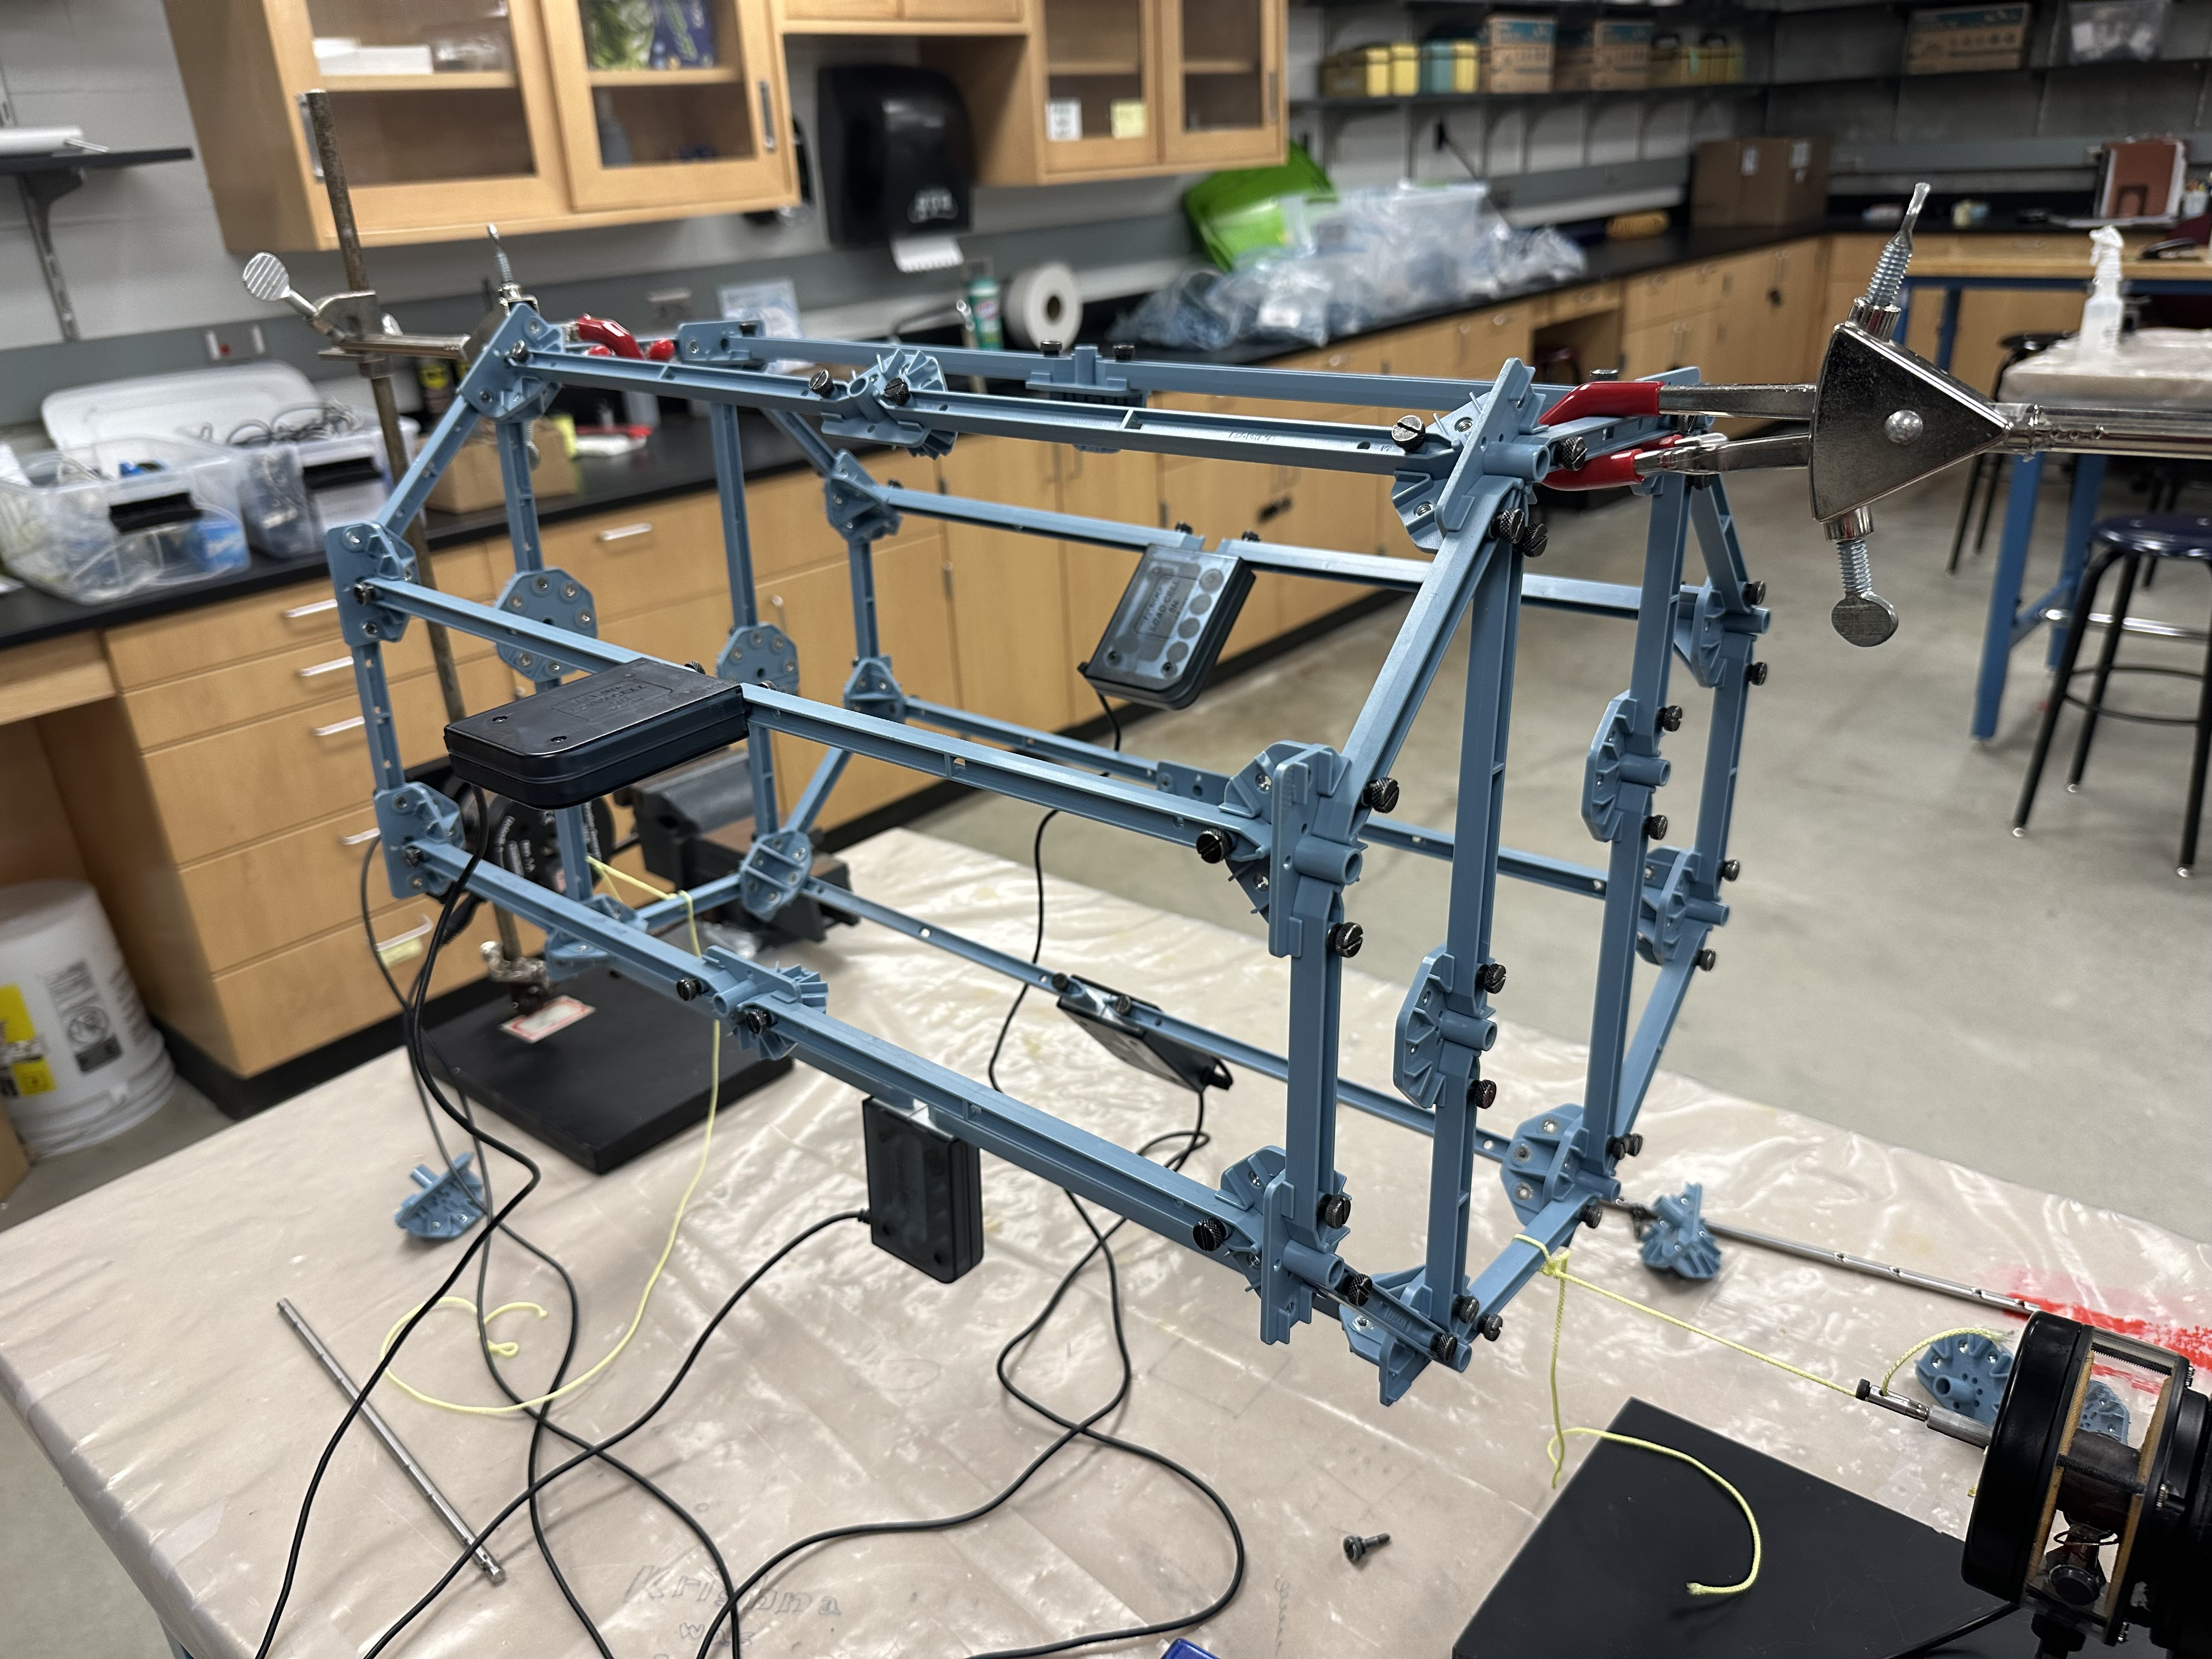
\includegraphics[width=4in]{images/IMG_1312}
	\caption{An overview of the fully assembled fuselage apparatus in test \num{1}.}
	\label{fig:test1_app_1}
\end{figure}

\begin{figure}[htbp]
	\centering
	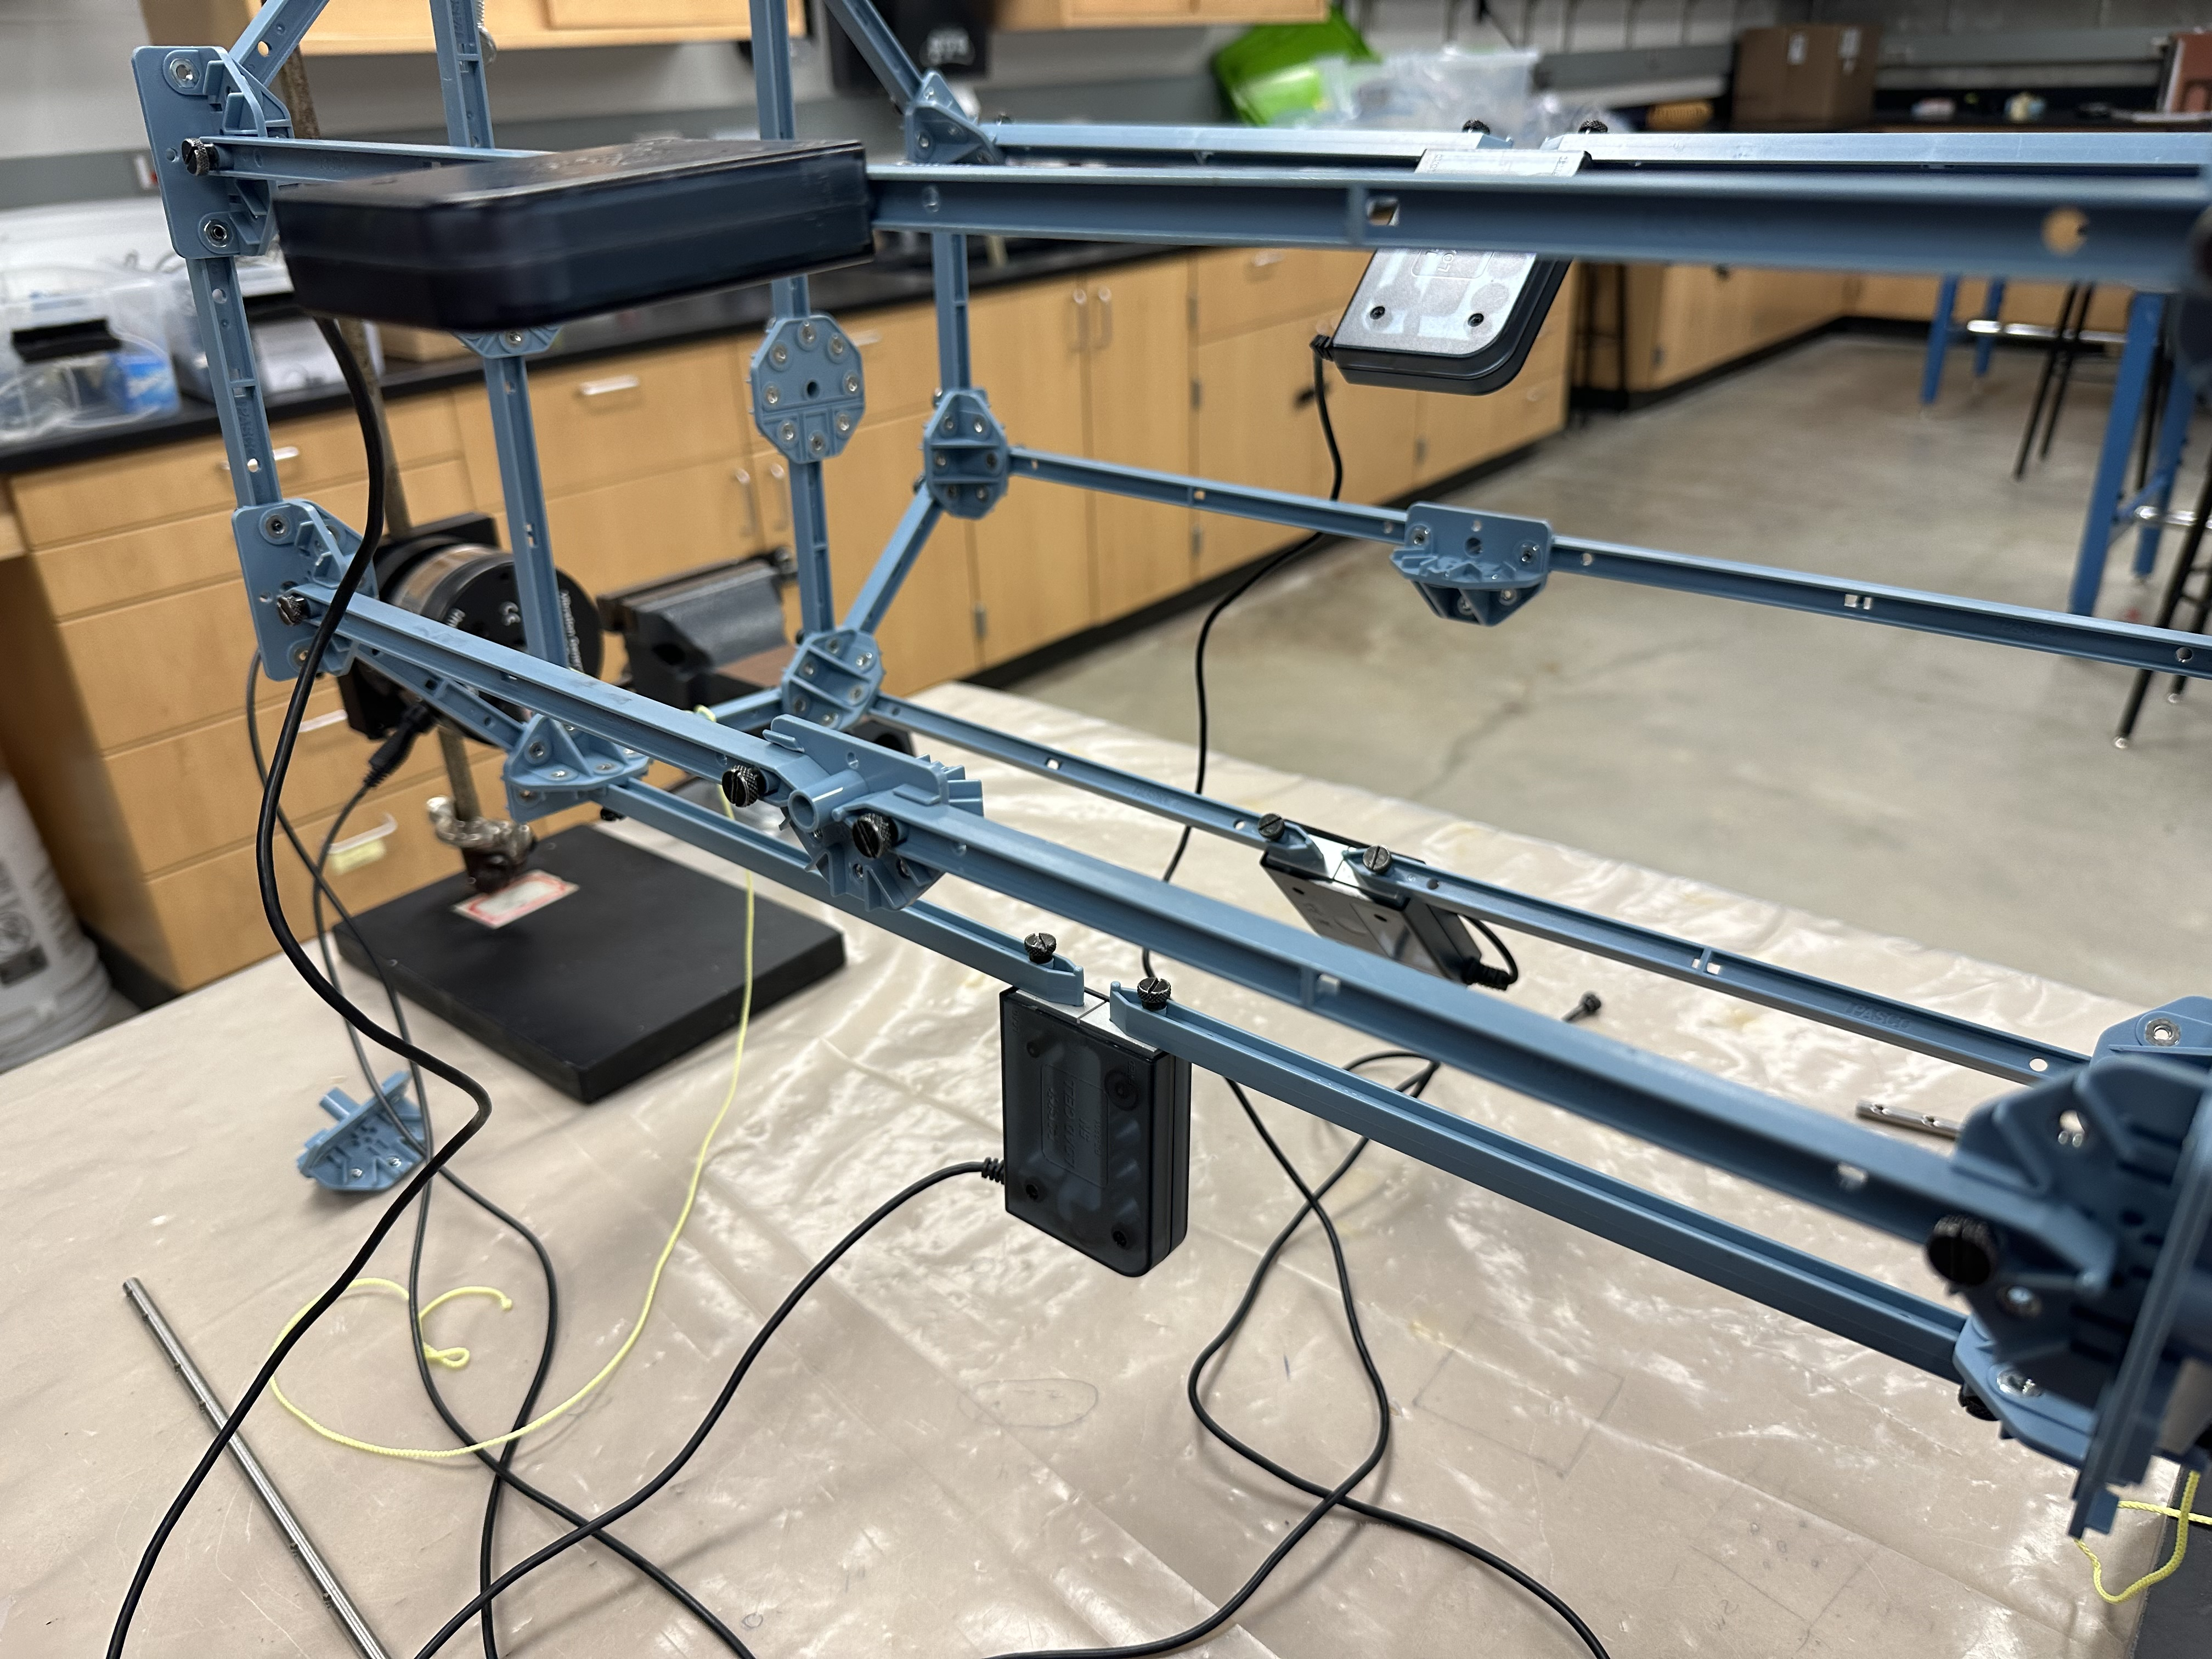
\includegraphics[width=4in]{images/IMG_1313}
	\caption{A close-up image showing the location of the four load cells in the fuselage structure in the test \num{1} configuration.}
	\label{fig:test1_app_2}
\end{figure}

\begin{figure}[htbp]
	\centering
	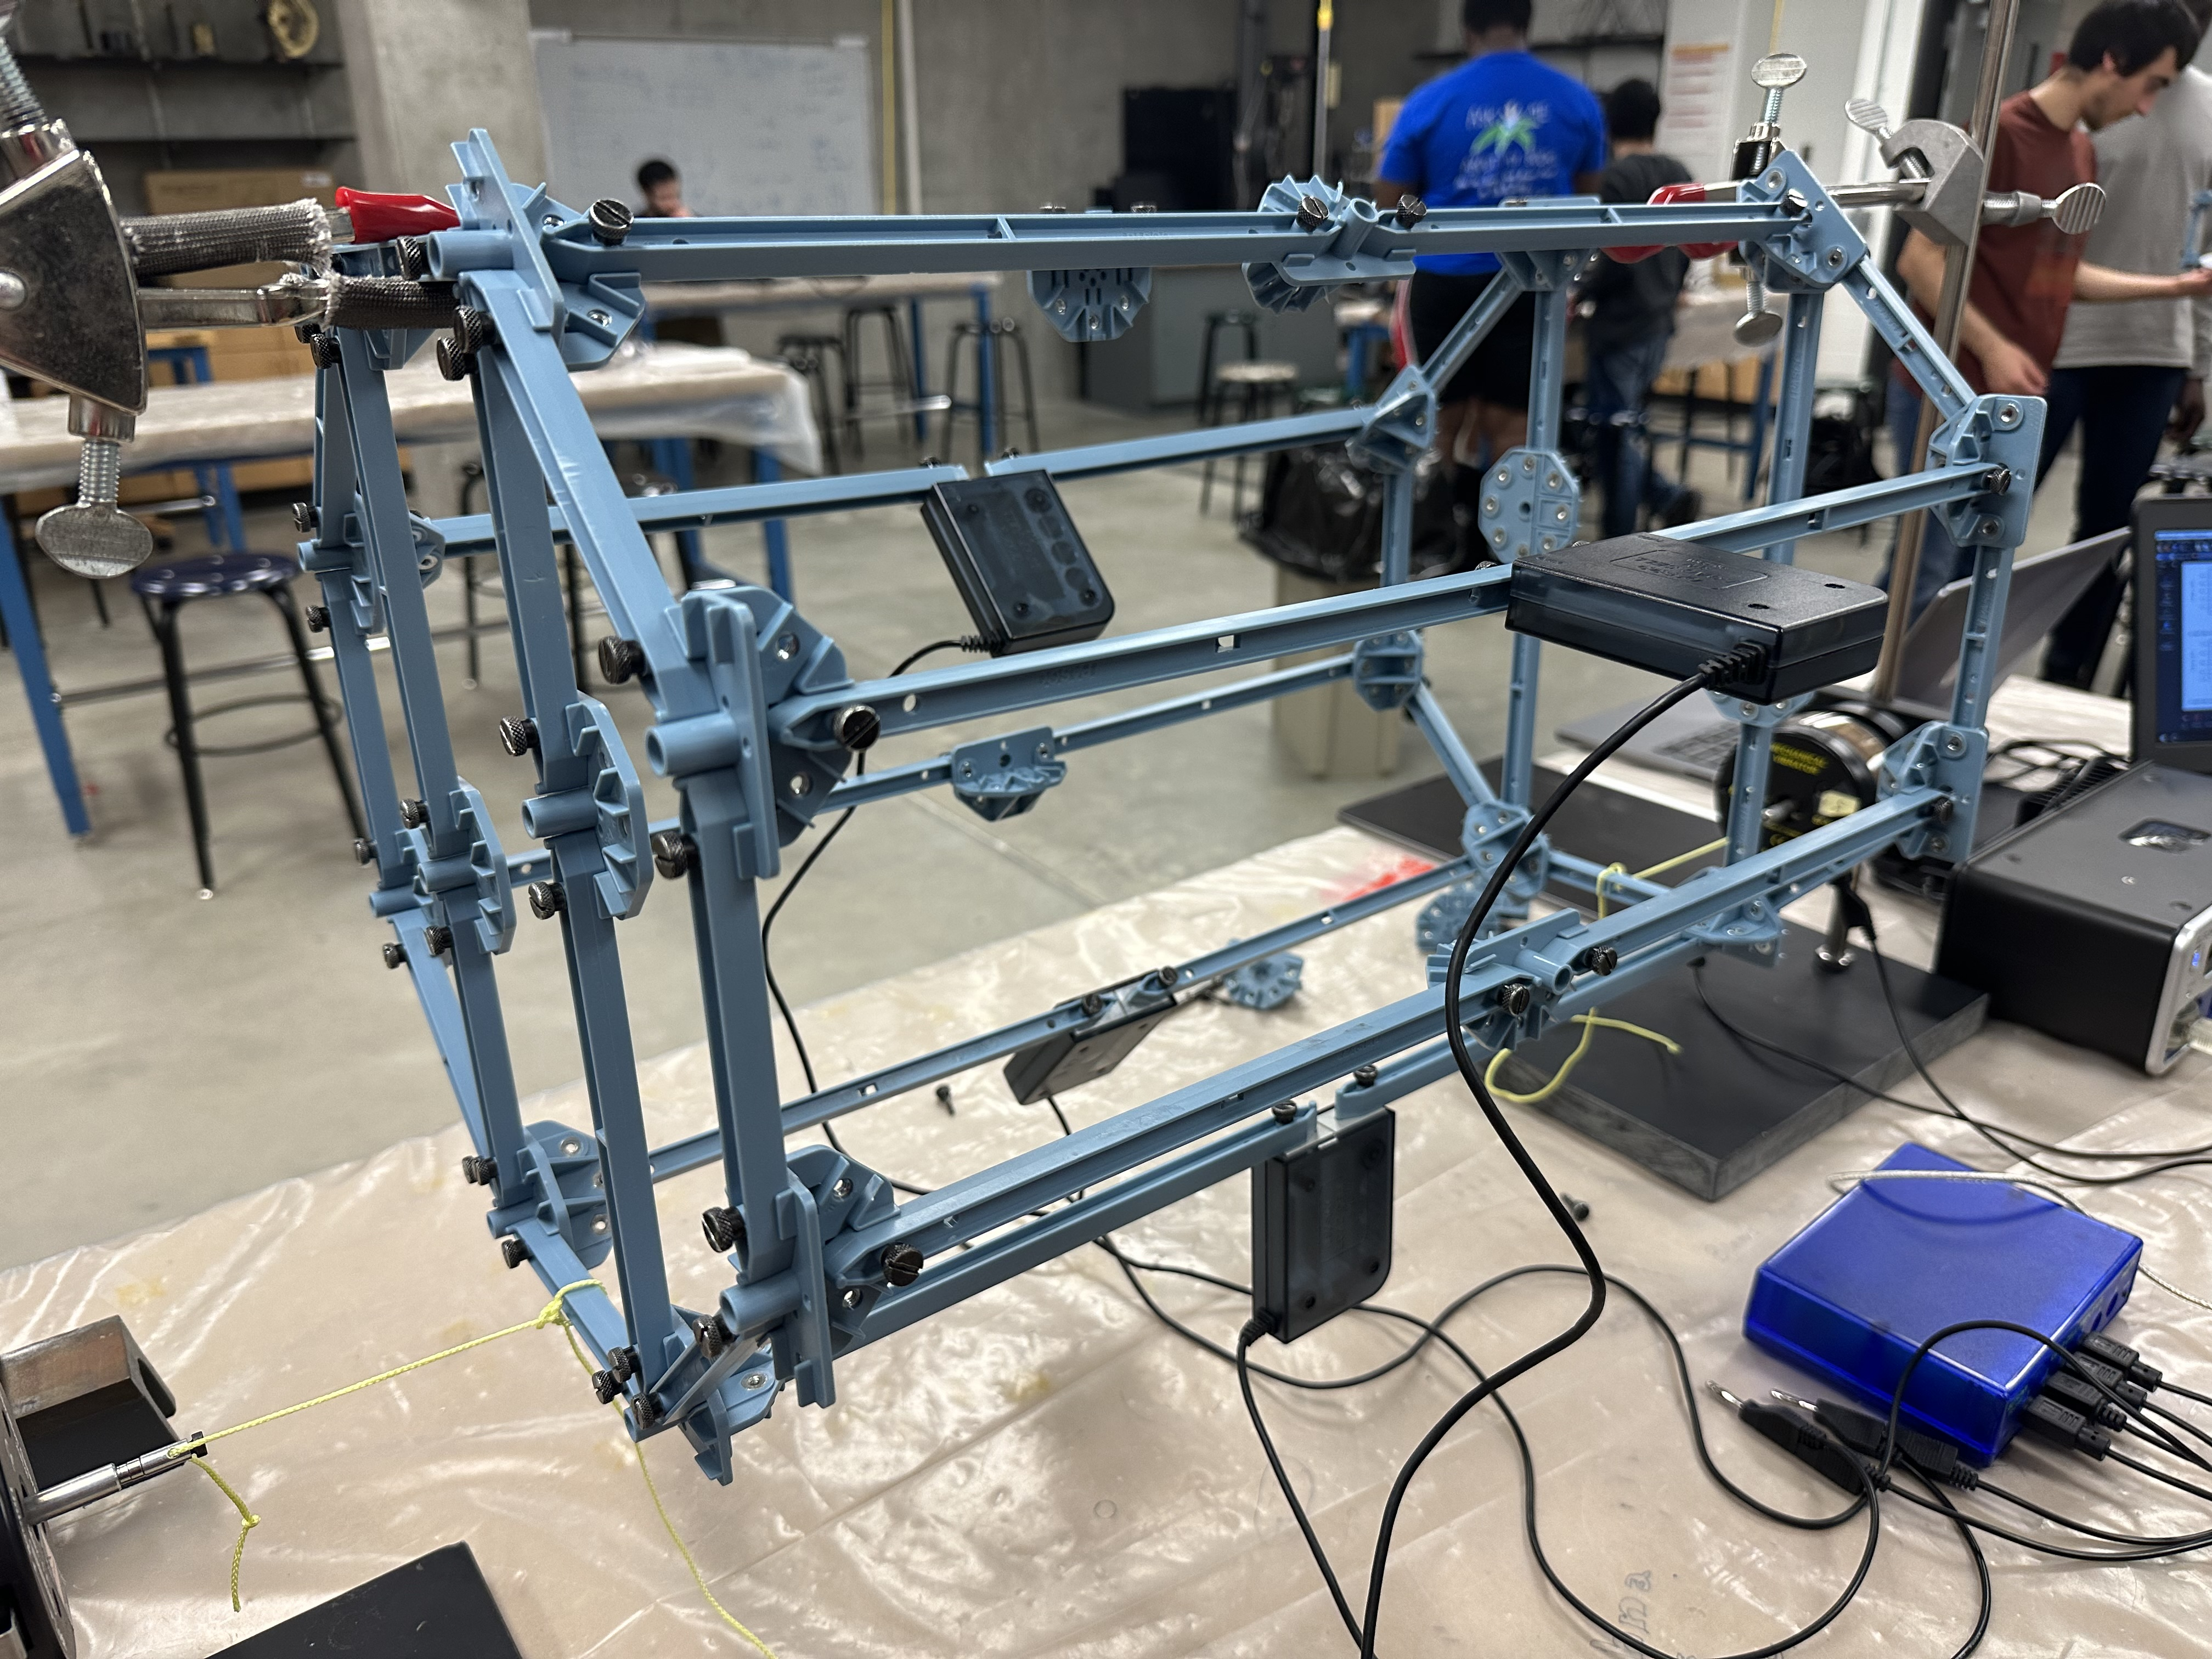
\includegraphics[width=4in]{images/IMG_1314}
	\caption{Another angle of the entire fuselage apparatus in the test \num{1} configuration.}
	\label{fig:test1_app_3}
\end{figure}

\begin{figure}[htbp]
	\centering
	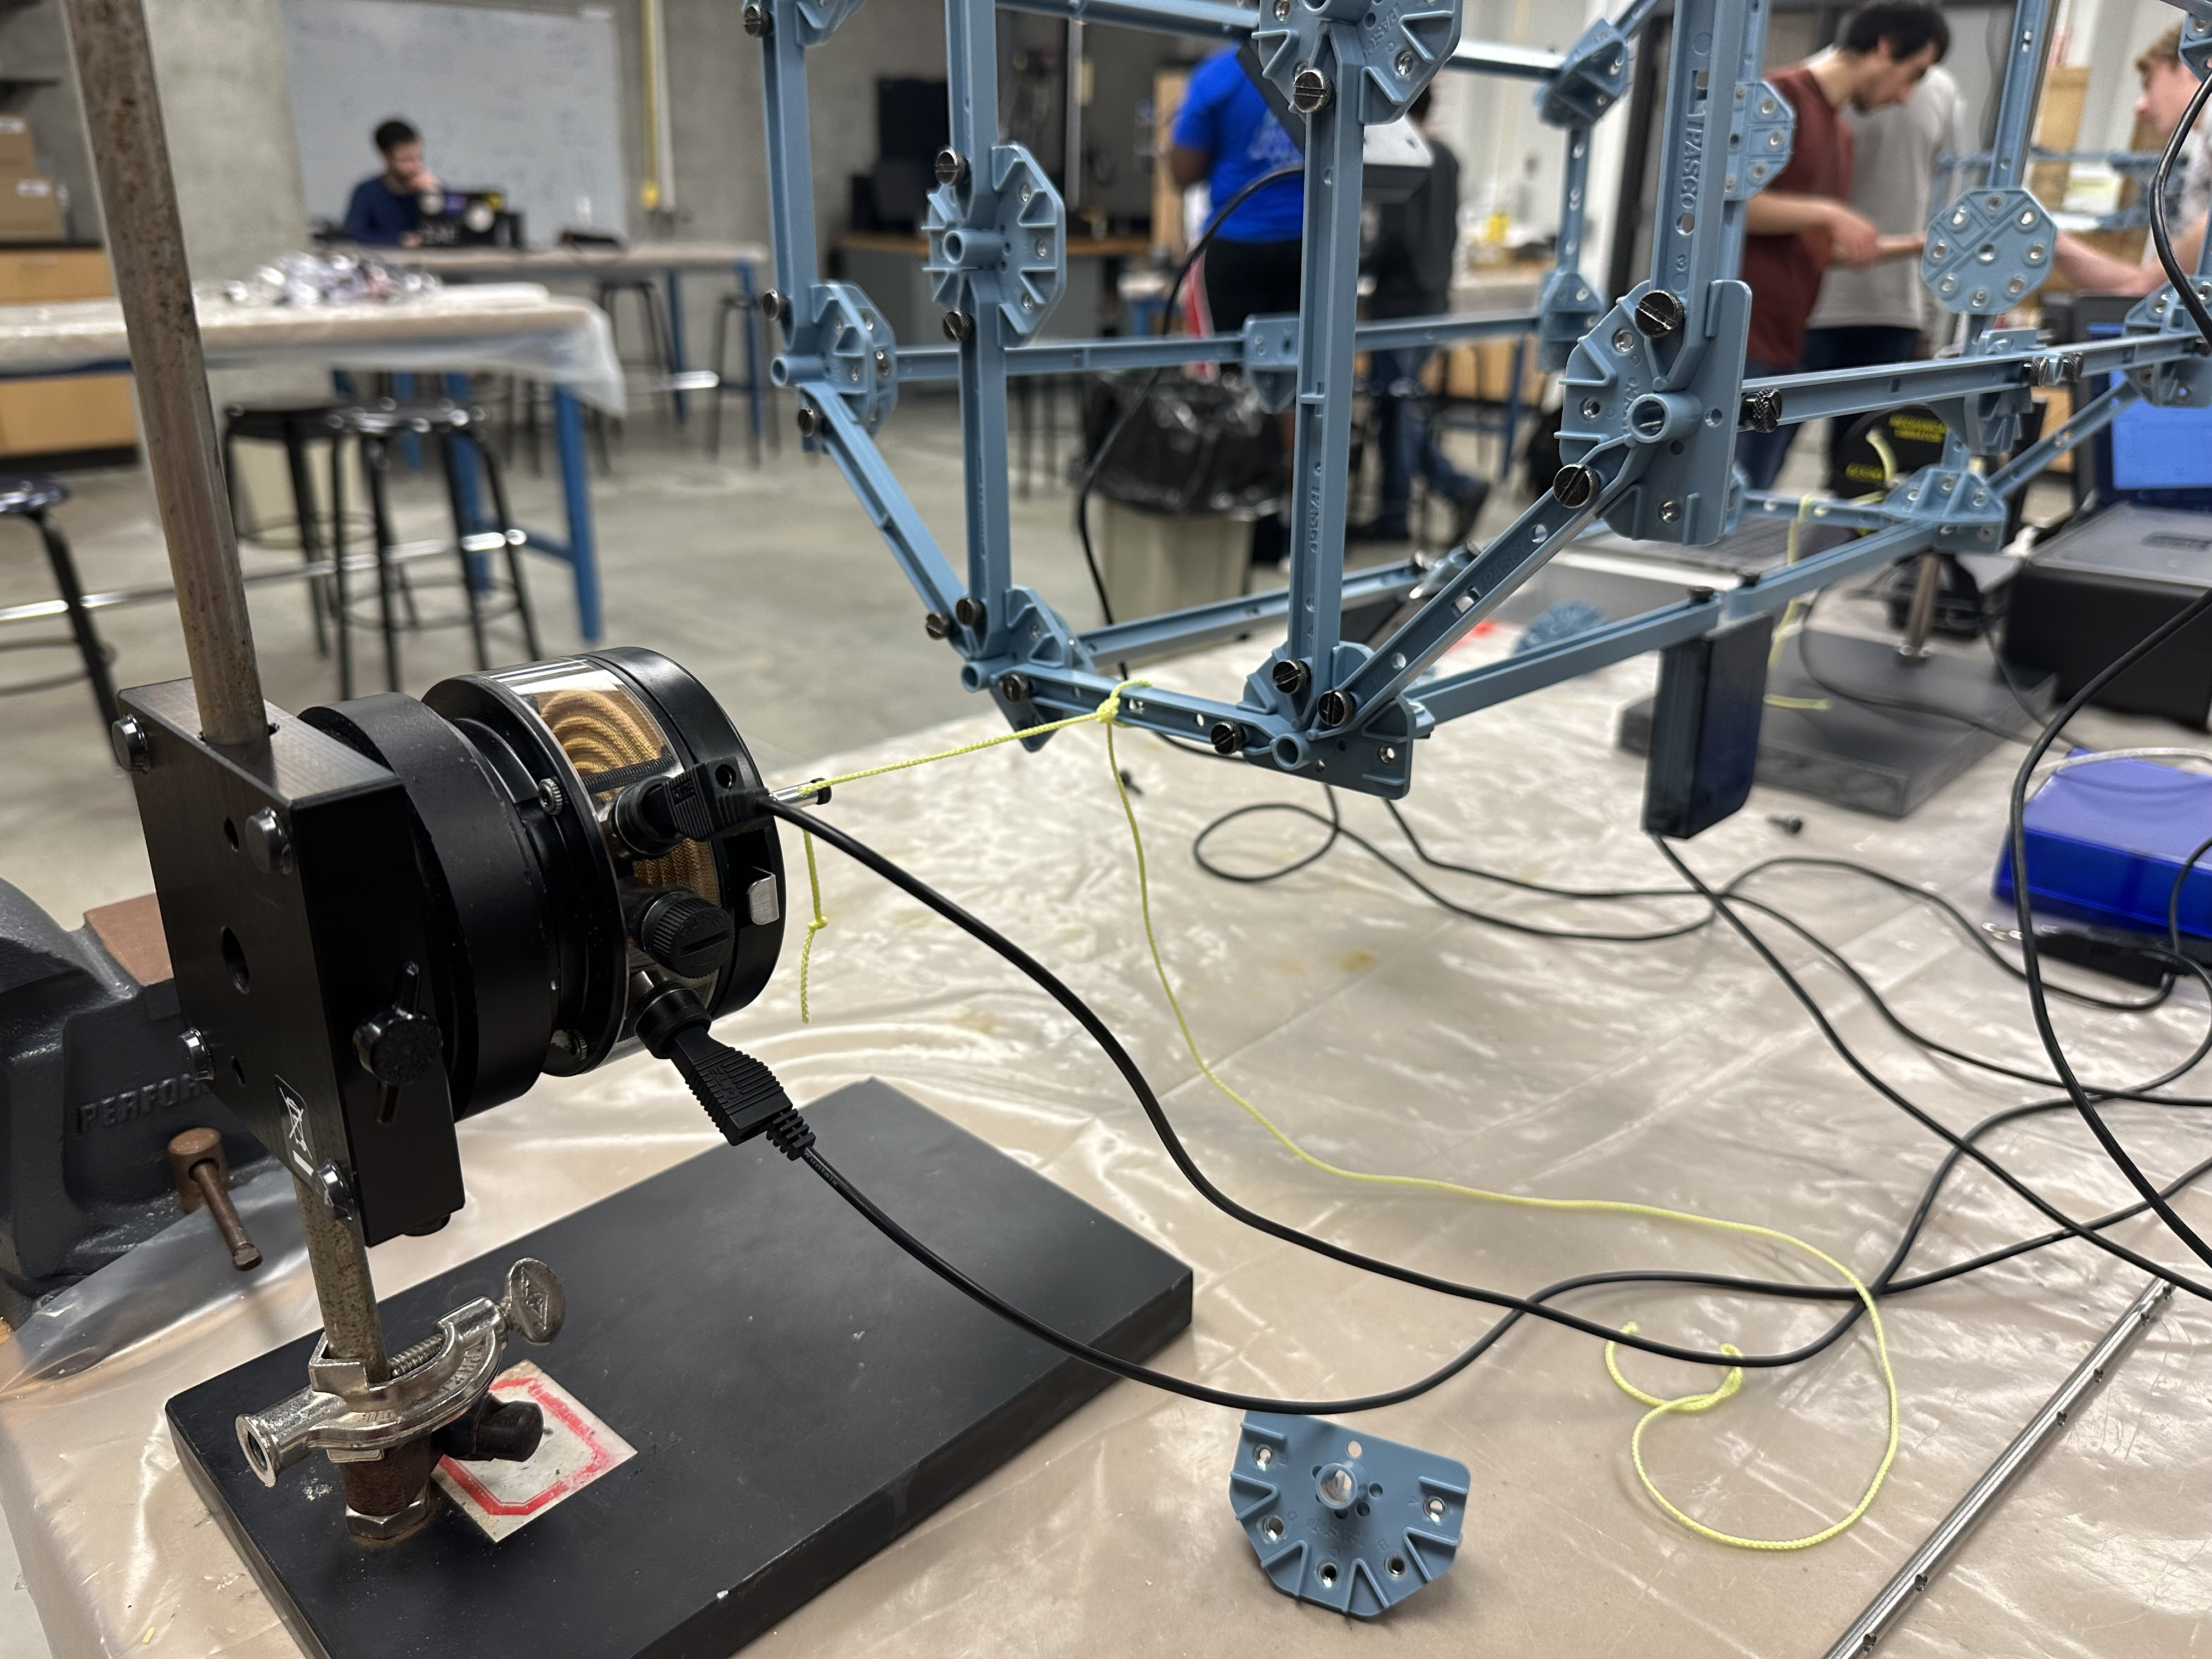
\includegraphics[width=4in]{images/IMG_1315}
	\caption{A close-up image of the configuration of the wave driver on the left-side of the fuselage apparatus in the test \num{1} configuration.}
	\label{fig:test1_app_4}
\end{figure}

\begin{figure}[htbp]
	\centering
	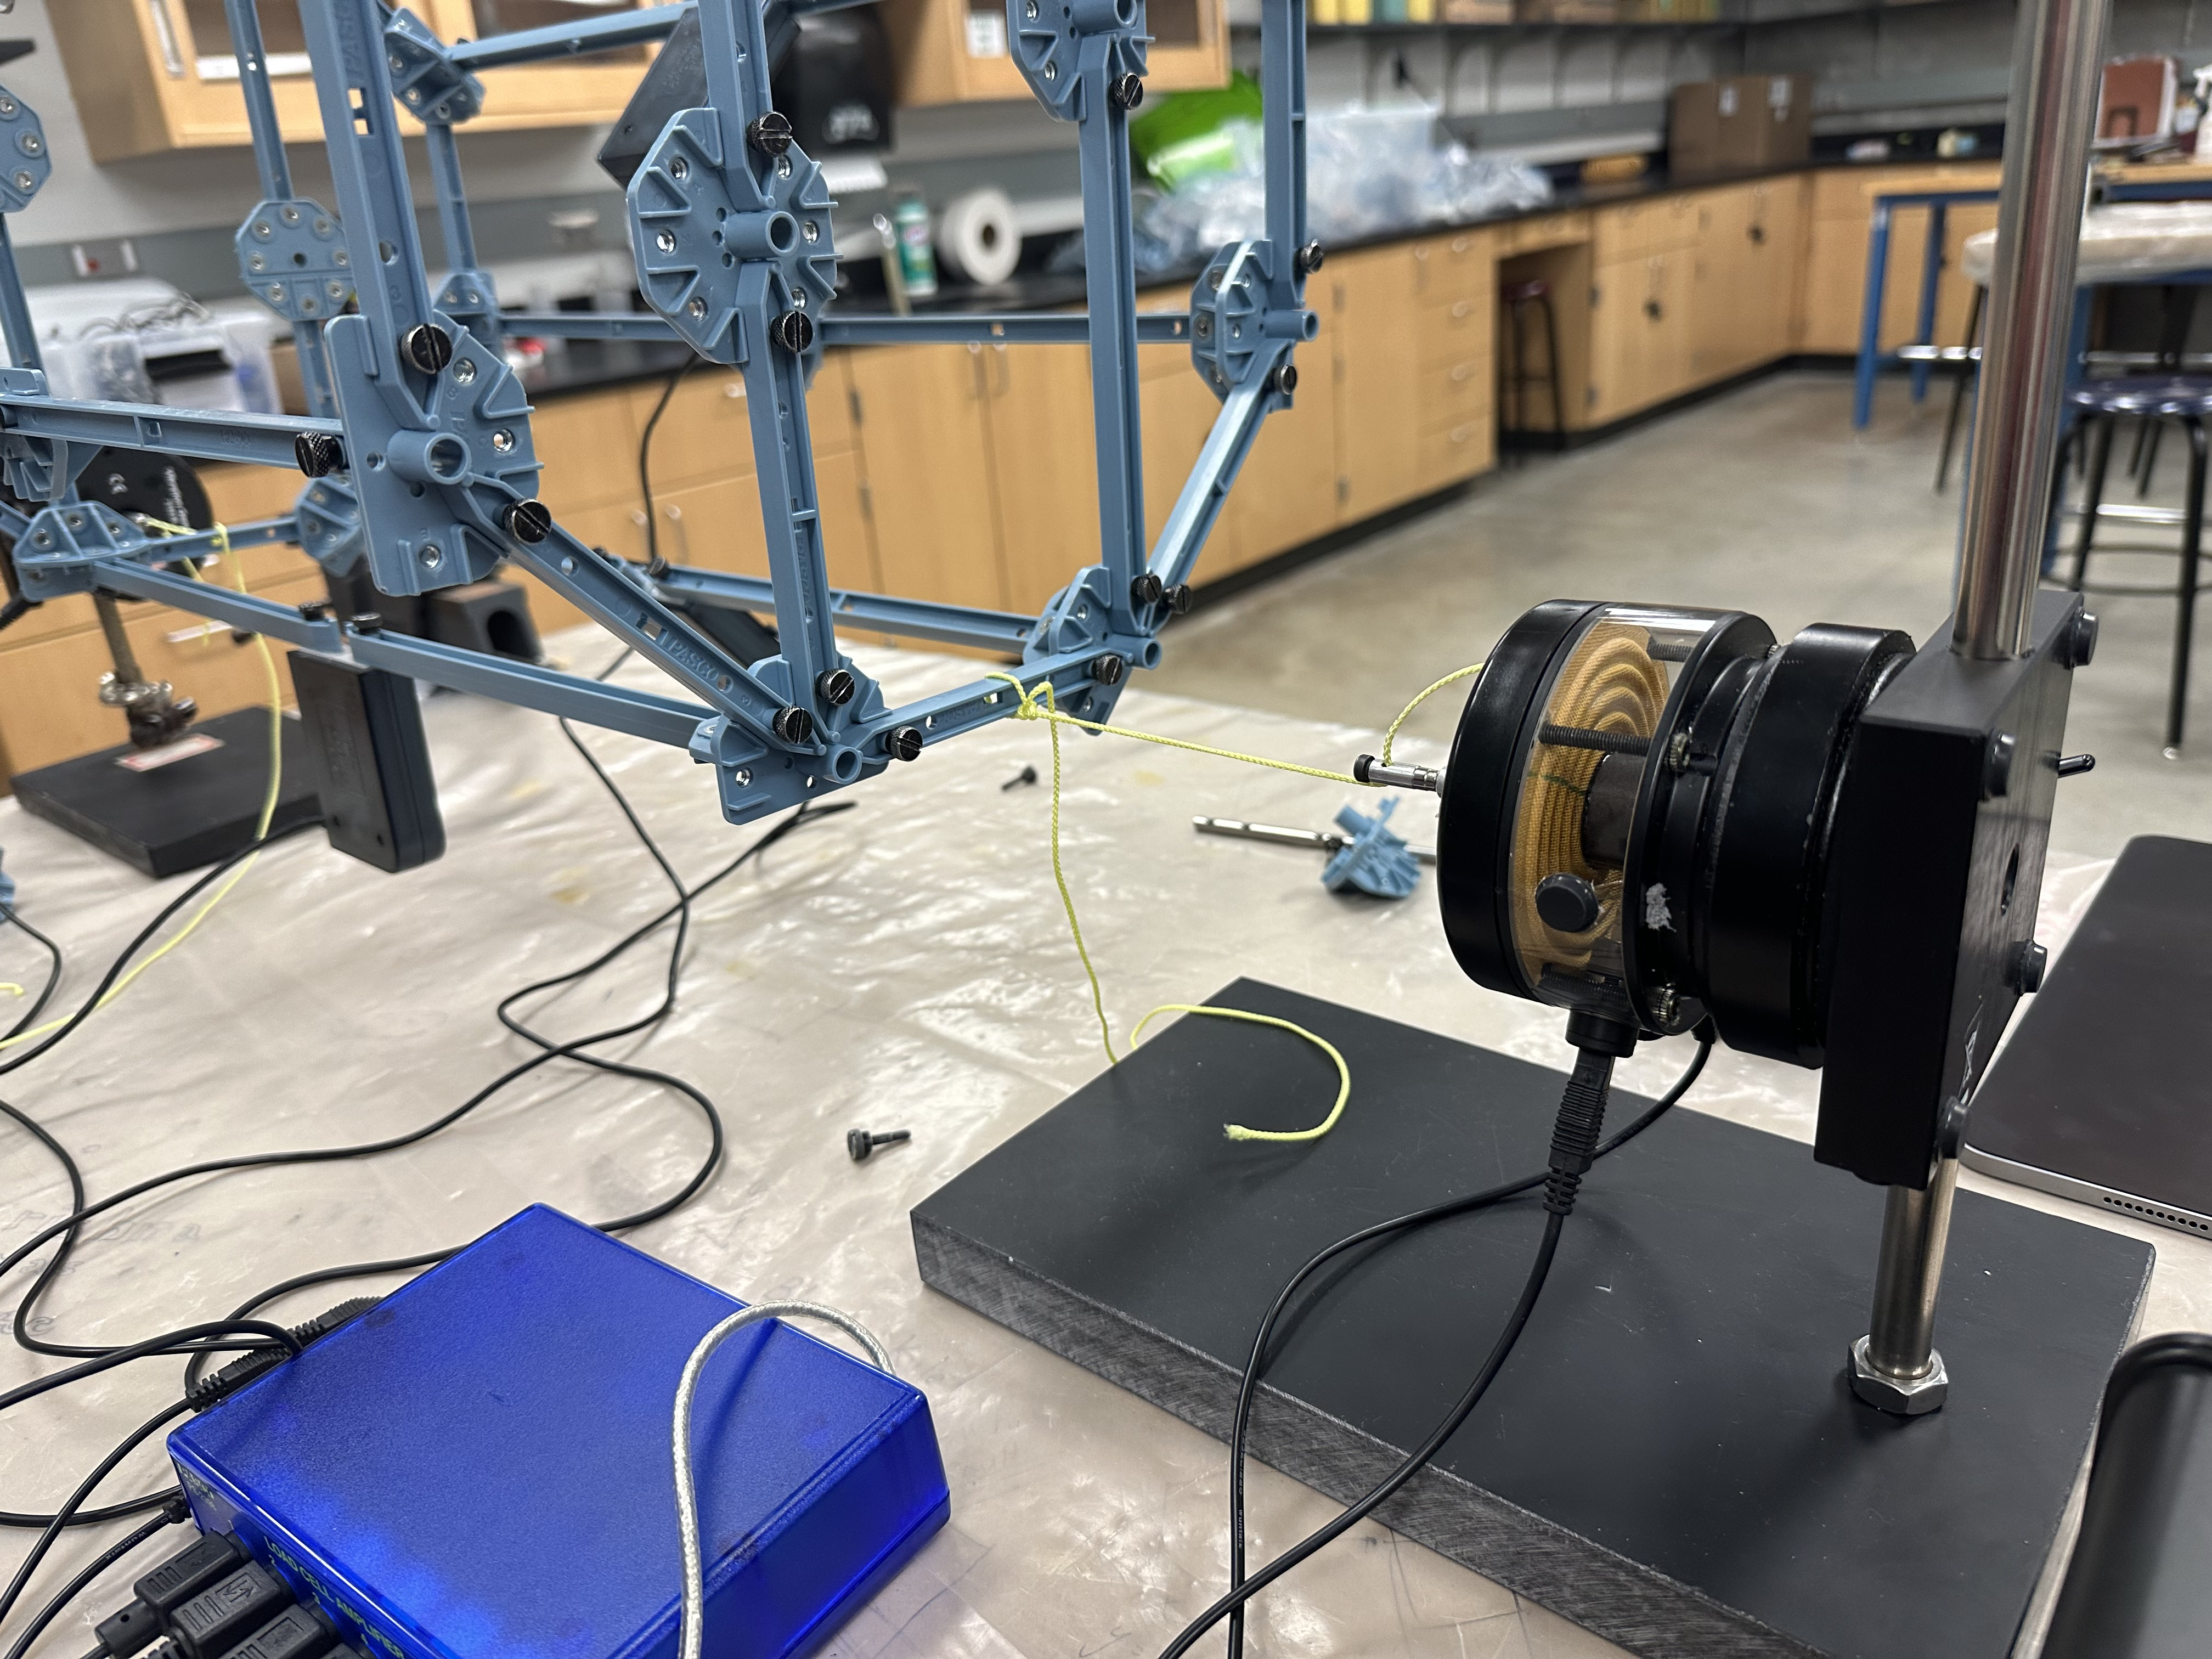
\includegraphics[width=4in]{images/IMG_1316}
	\caption{A close-up image of the configuration of the wave driver on the right-side of the fuselage apparatus in the test \num{1} configuration.}
	\label{fig:test1_app_5}
\end{figure}

\begin{figure}[htbp]
	\centering
	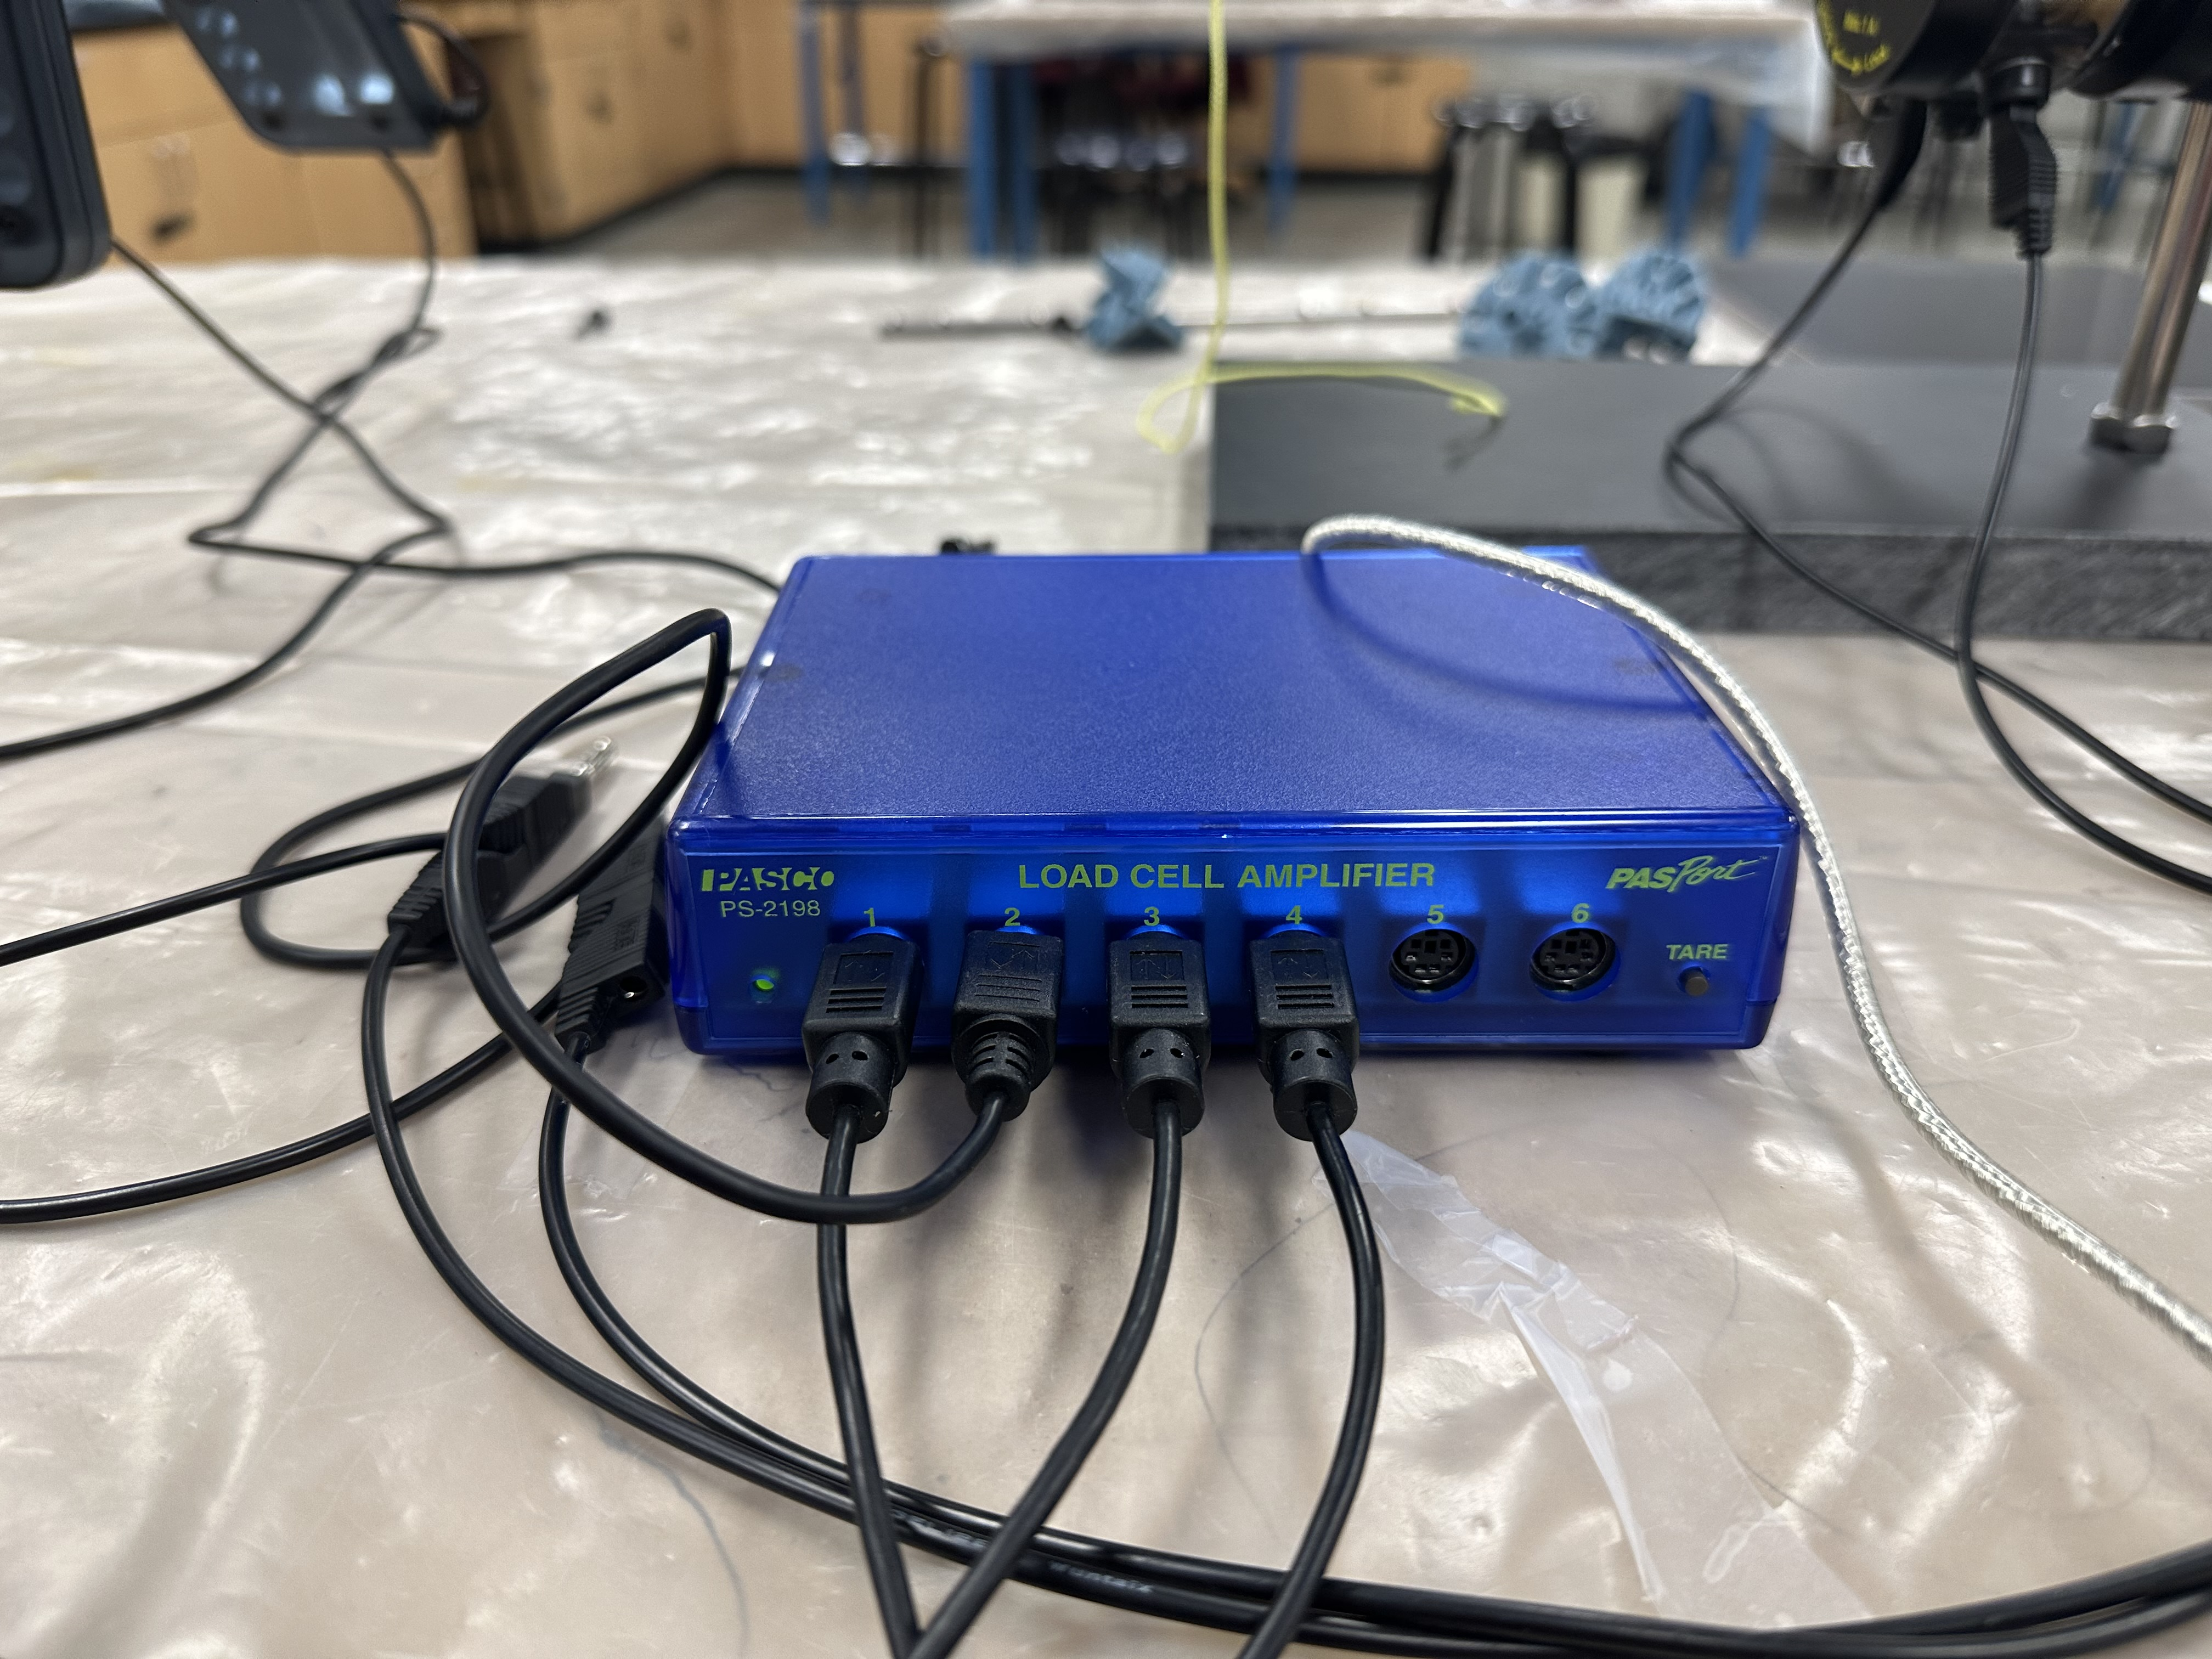
\includegraphics[width=4in]{images/IMG_1317}
	\caption{The PASCO Load Cell Amplifier. This device is configured identically in both test configurations.}
	\label{fig:test1_app_6}
\end{figure}

\begin{figure}[htbp]
	\centering
	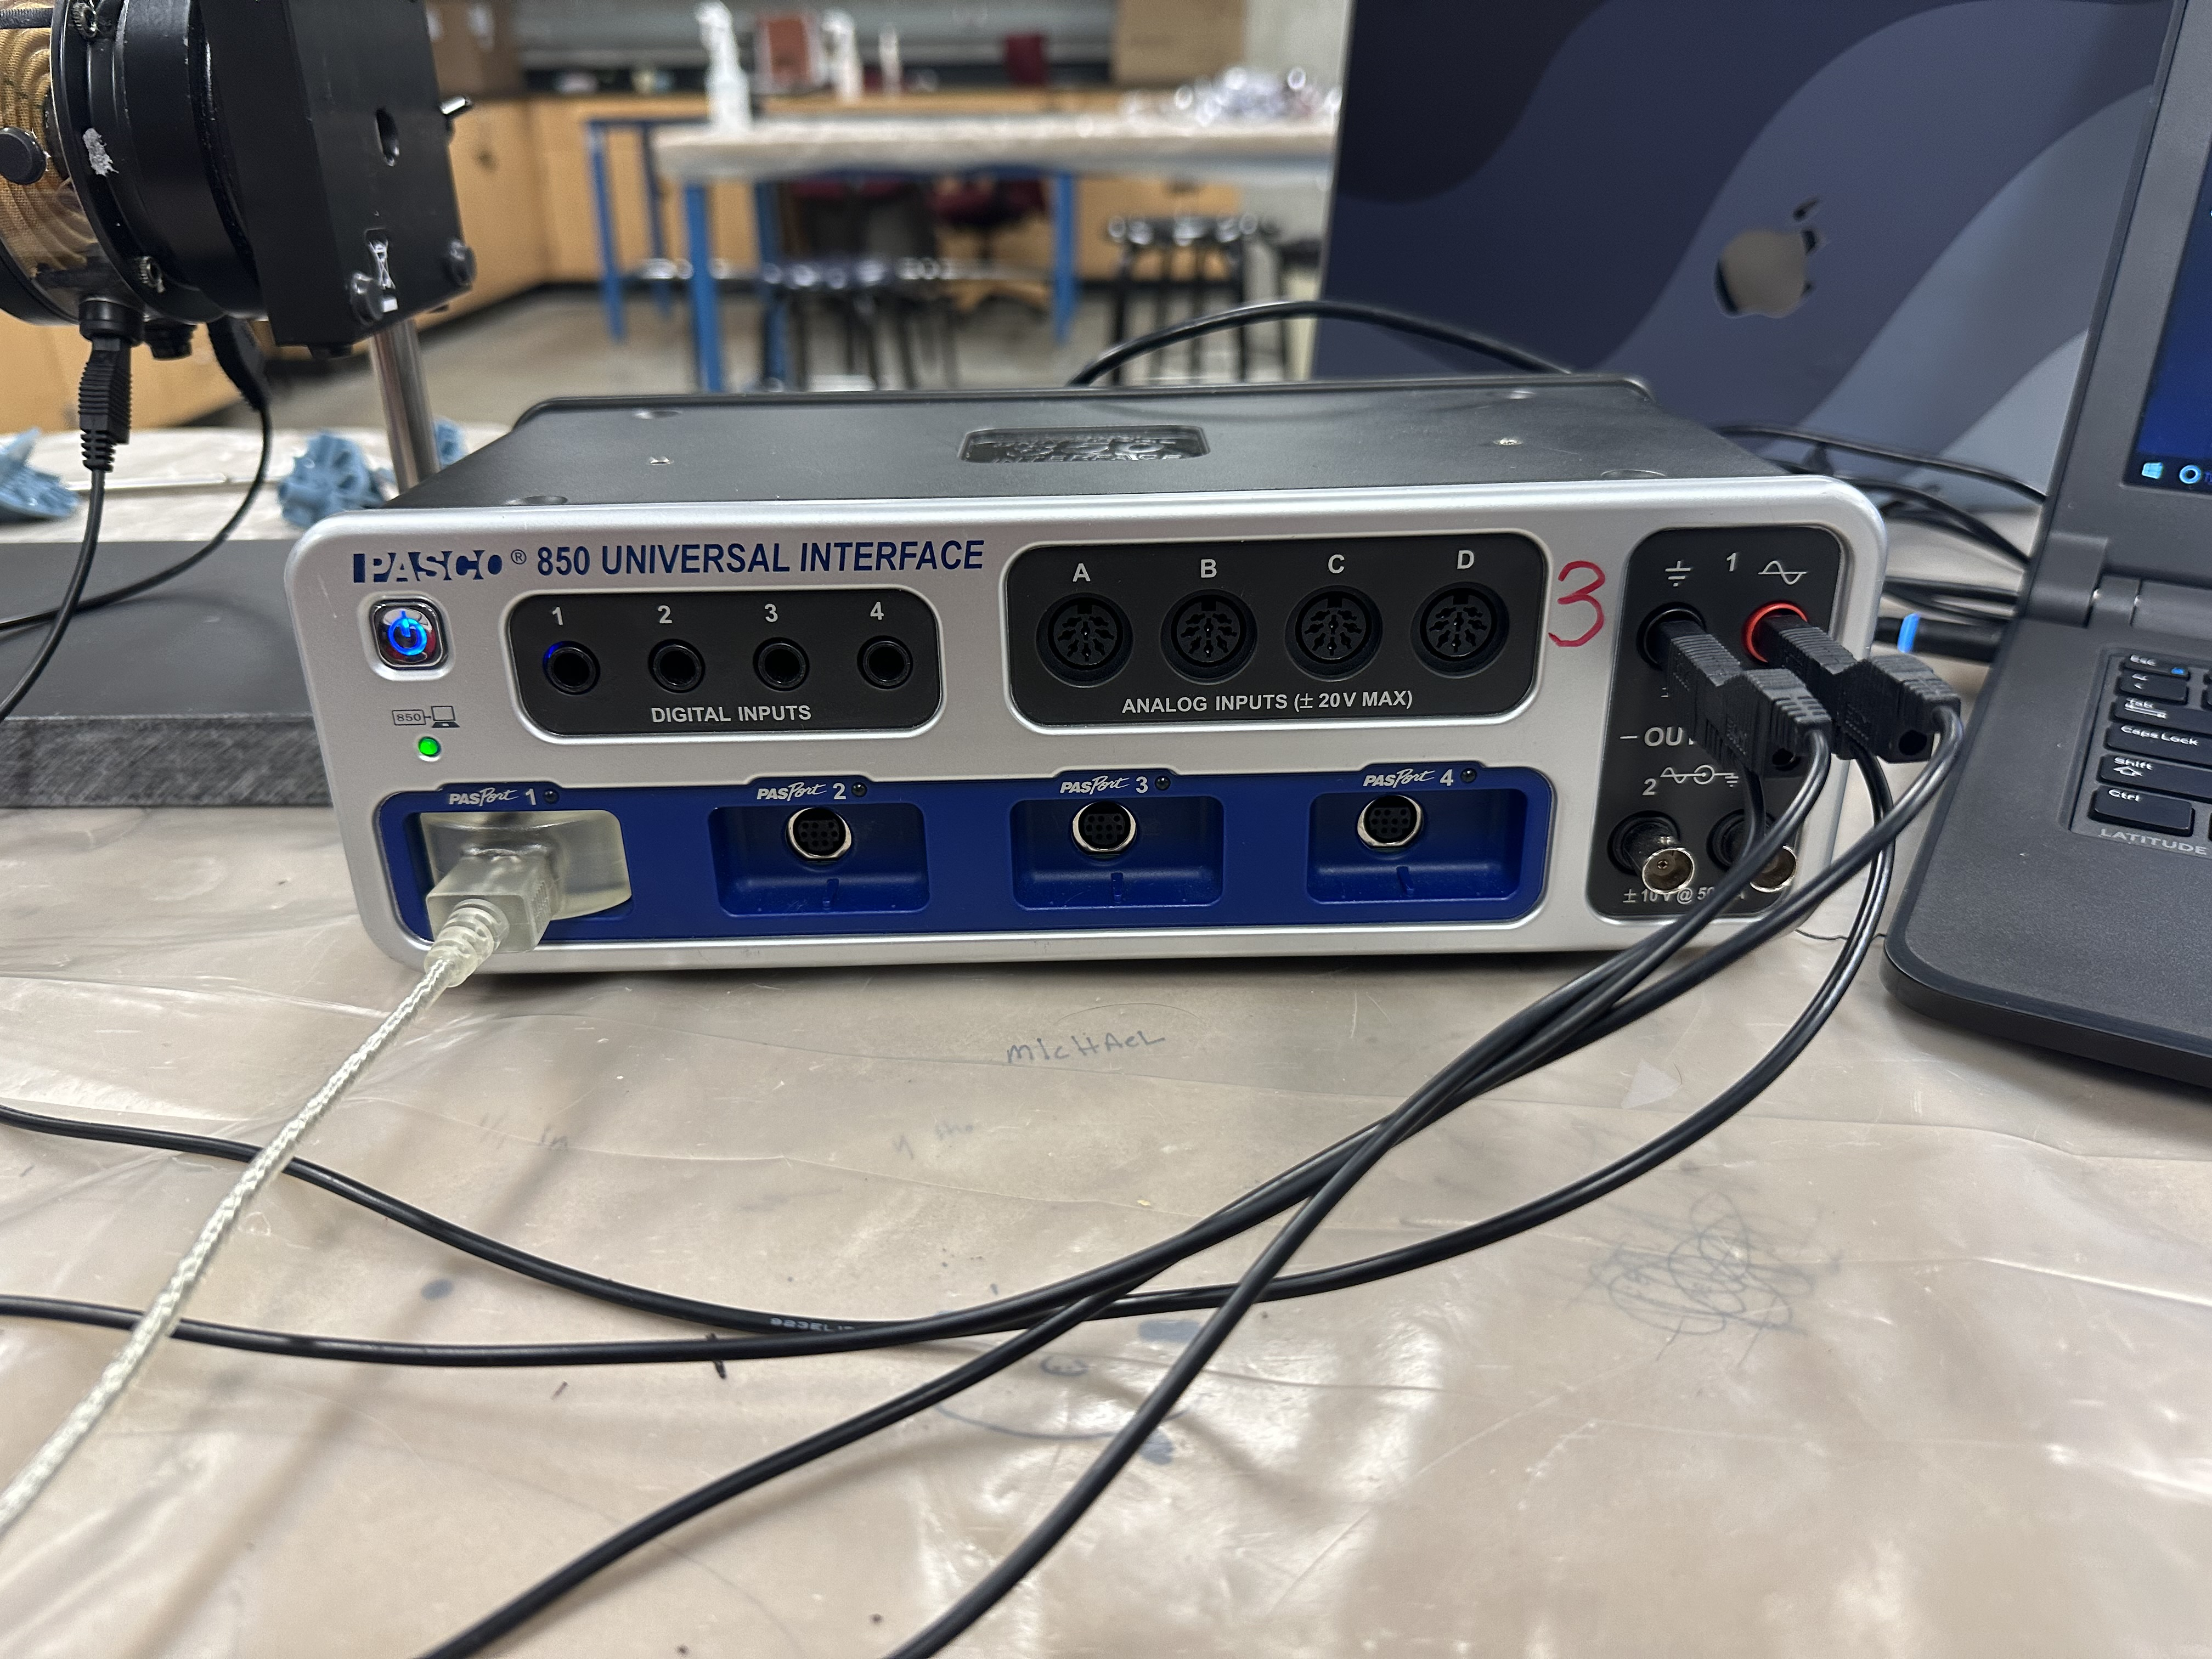
\includegraphics[width=4in]{images/IMG_1318}
	\caption{The PASCO 850 Universal Interface. This device is configured identically in both test configurations.}
	\label{fig:test1_app_7}
\end{figure}

\begin{figure}[htbp]
	\centering
	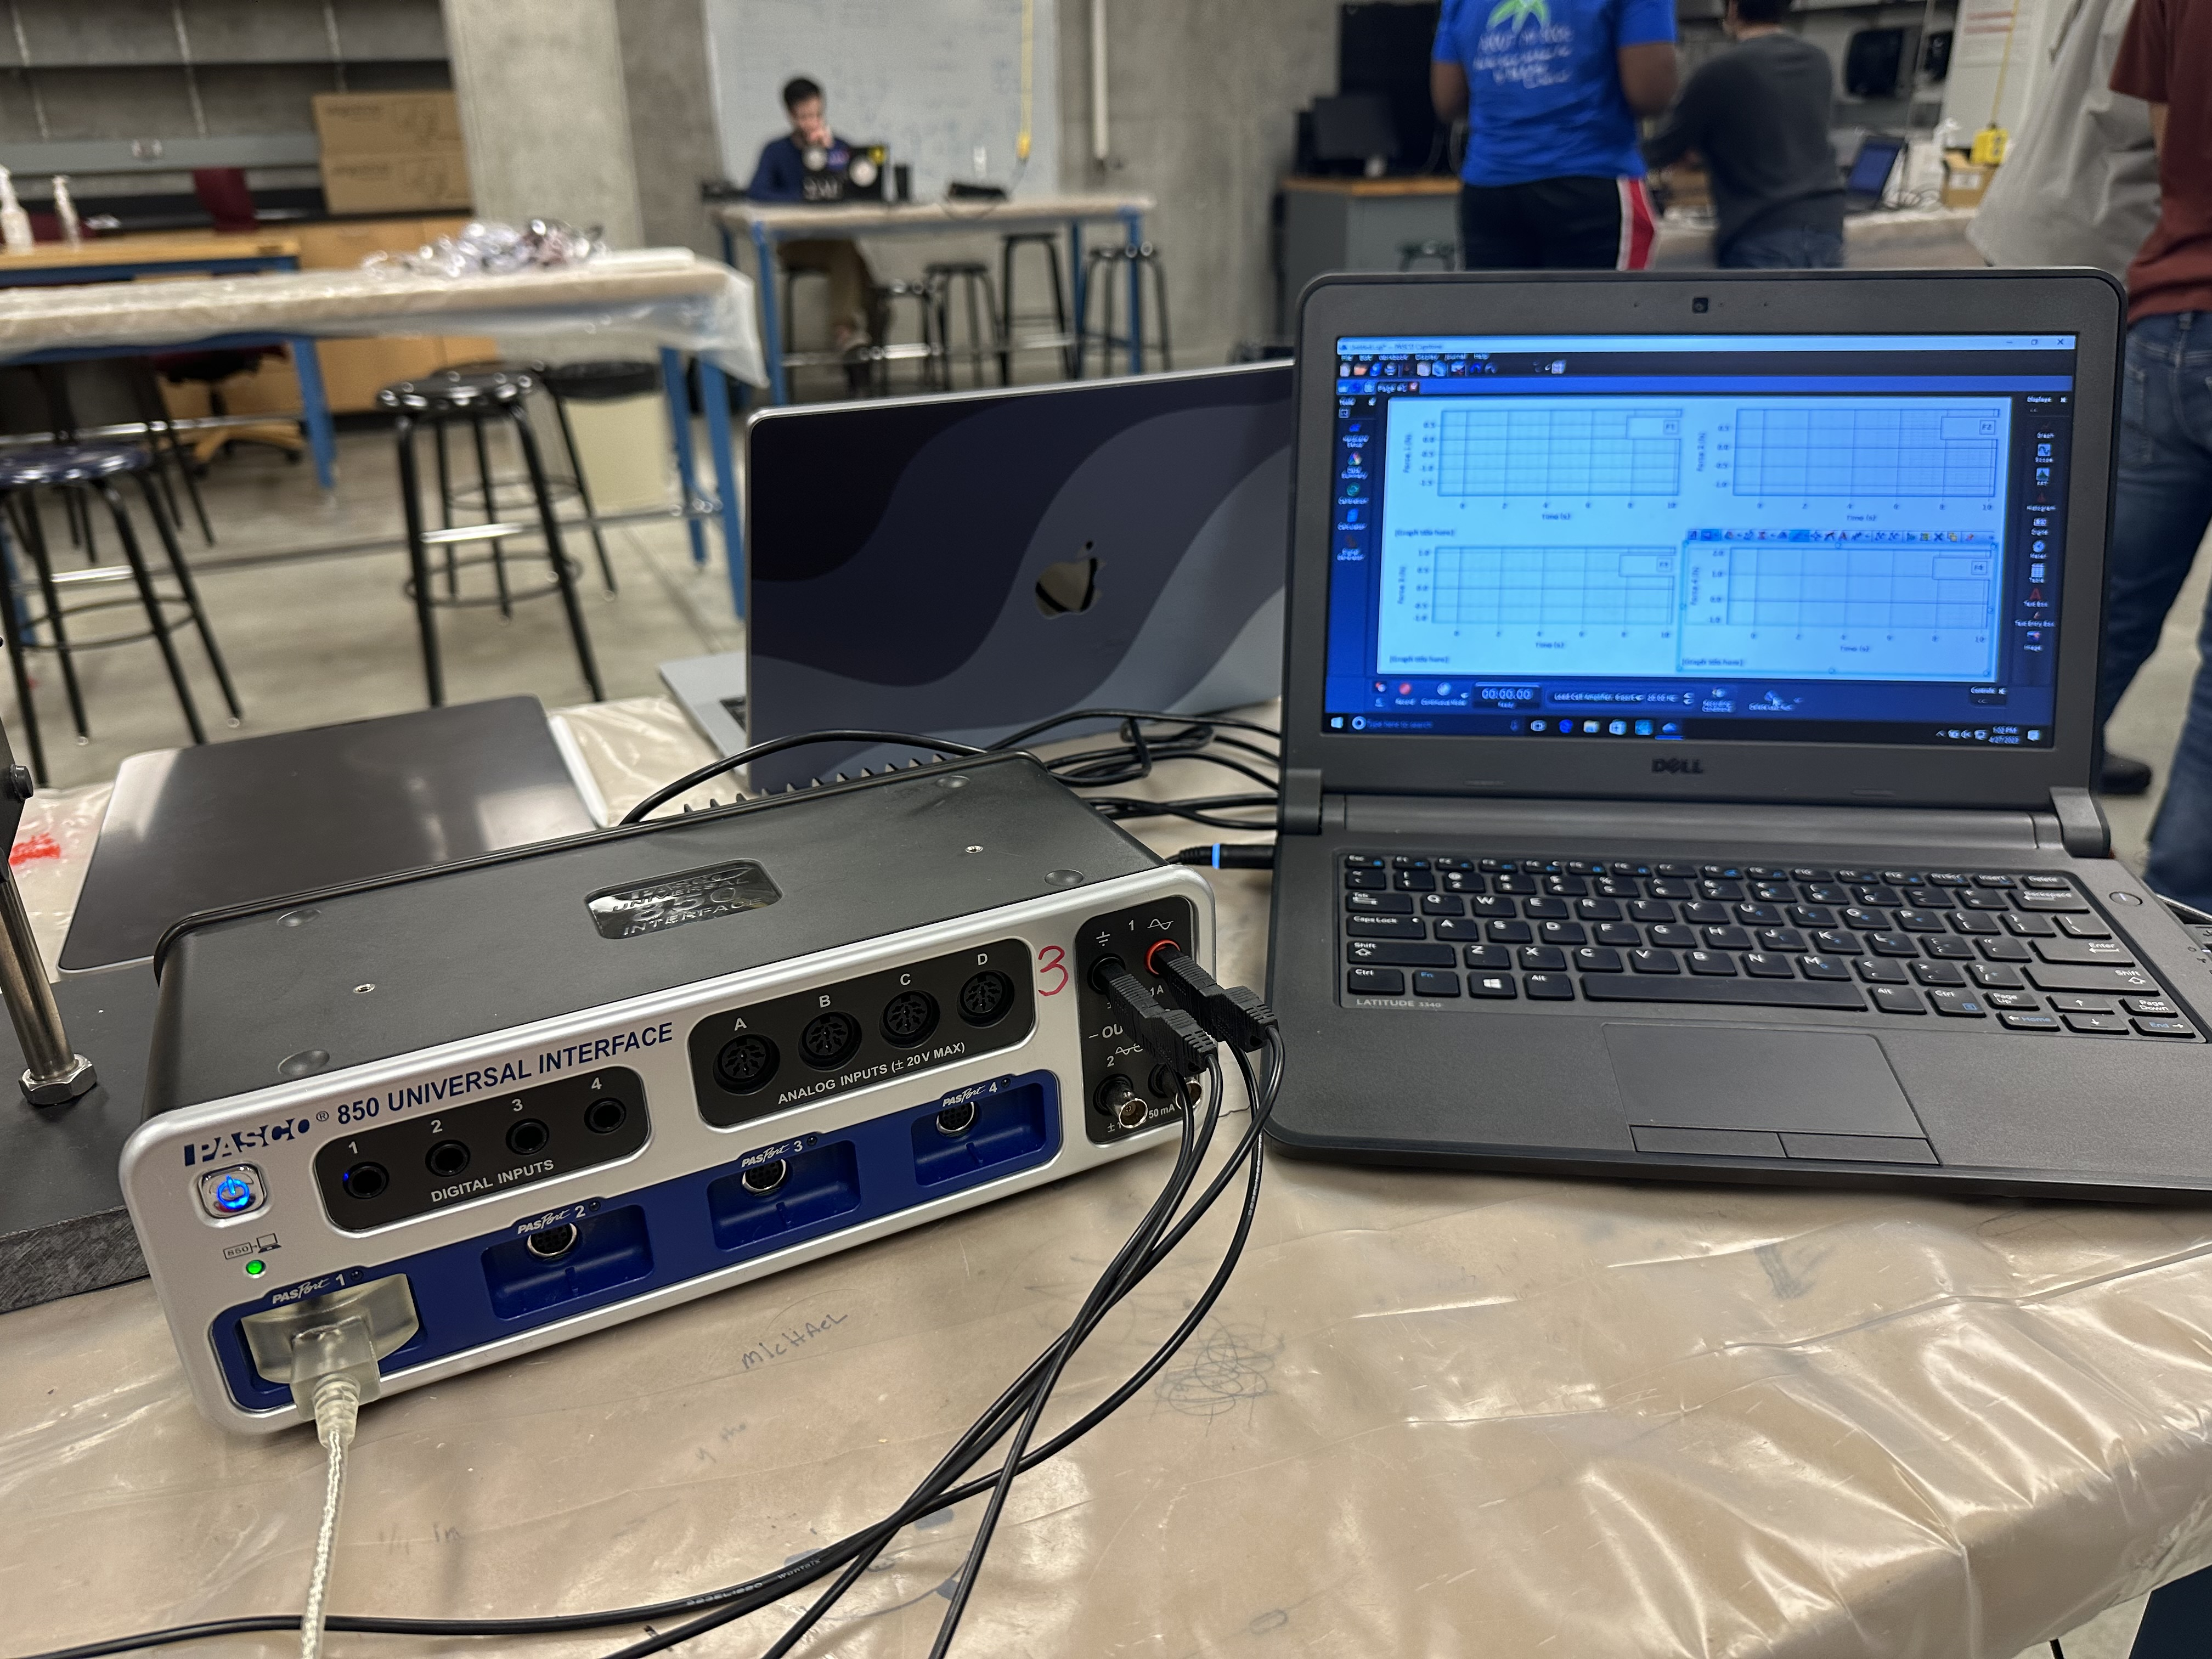
\includegraphics[width=4in]{images/IMG_1319}
	\caption{The PASCO 850 Universal Interface paired with a Dell laptop running the PASCO recording software.}
	\label{fig:test1_app_8}
\end{figure}

\begin{figure}[htbp]
	\centering
	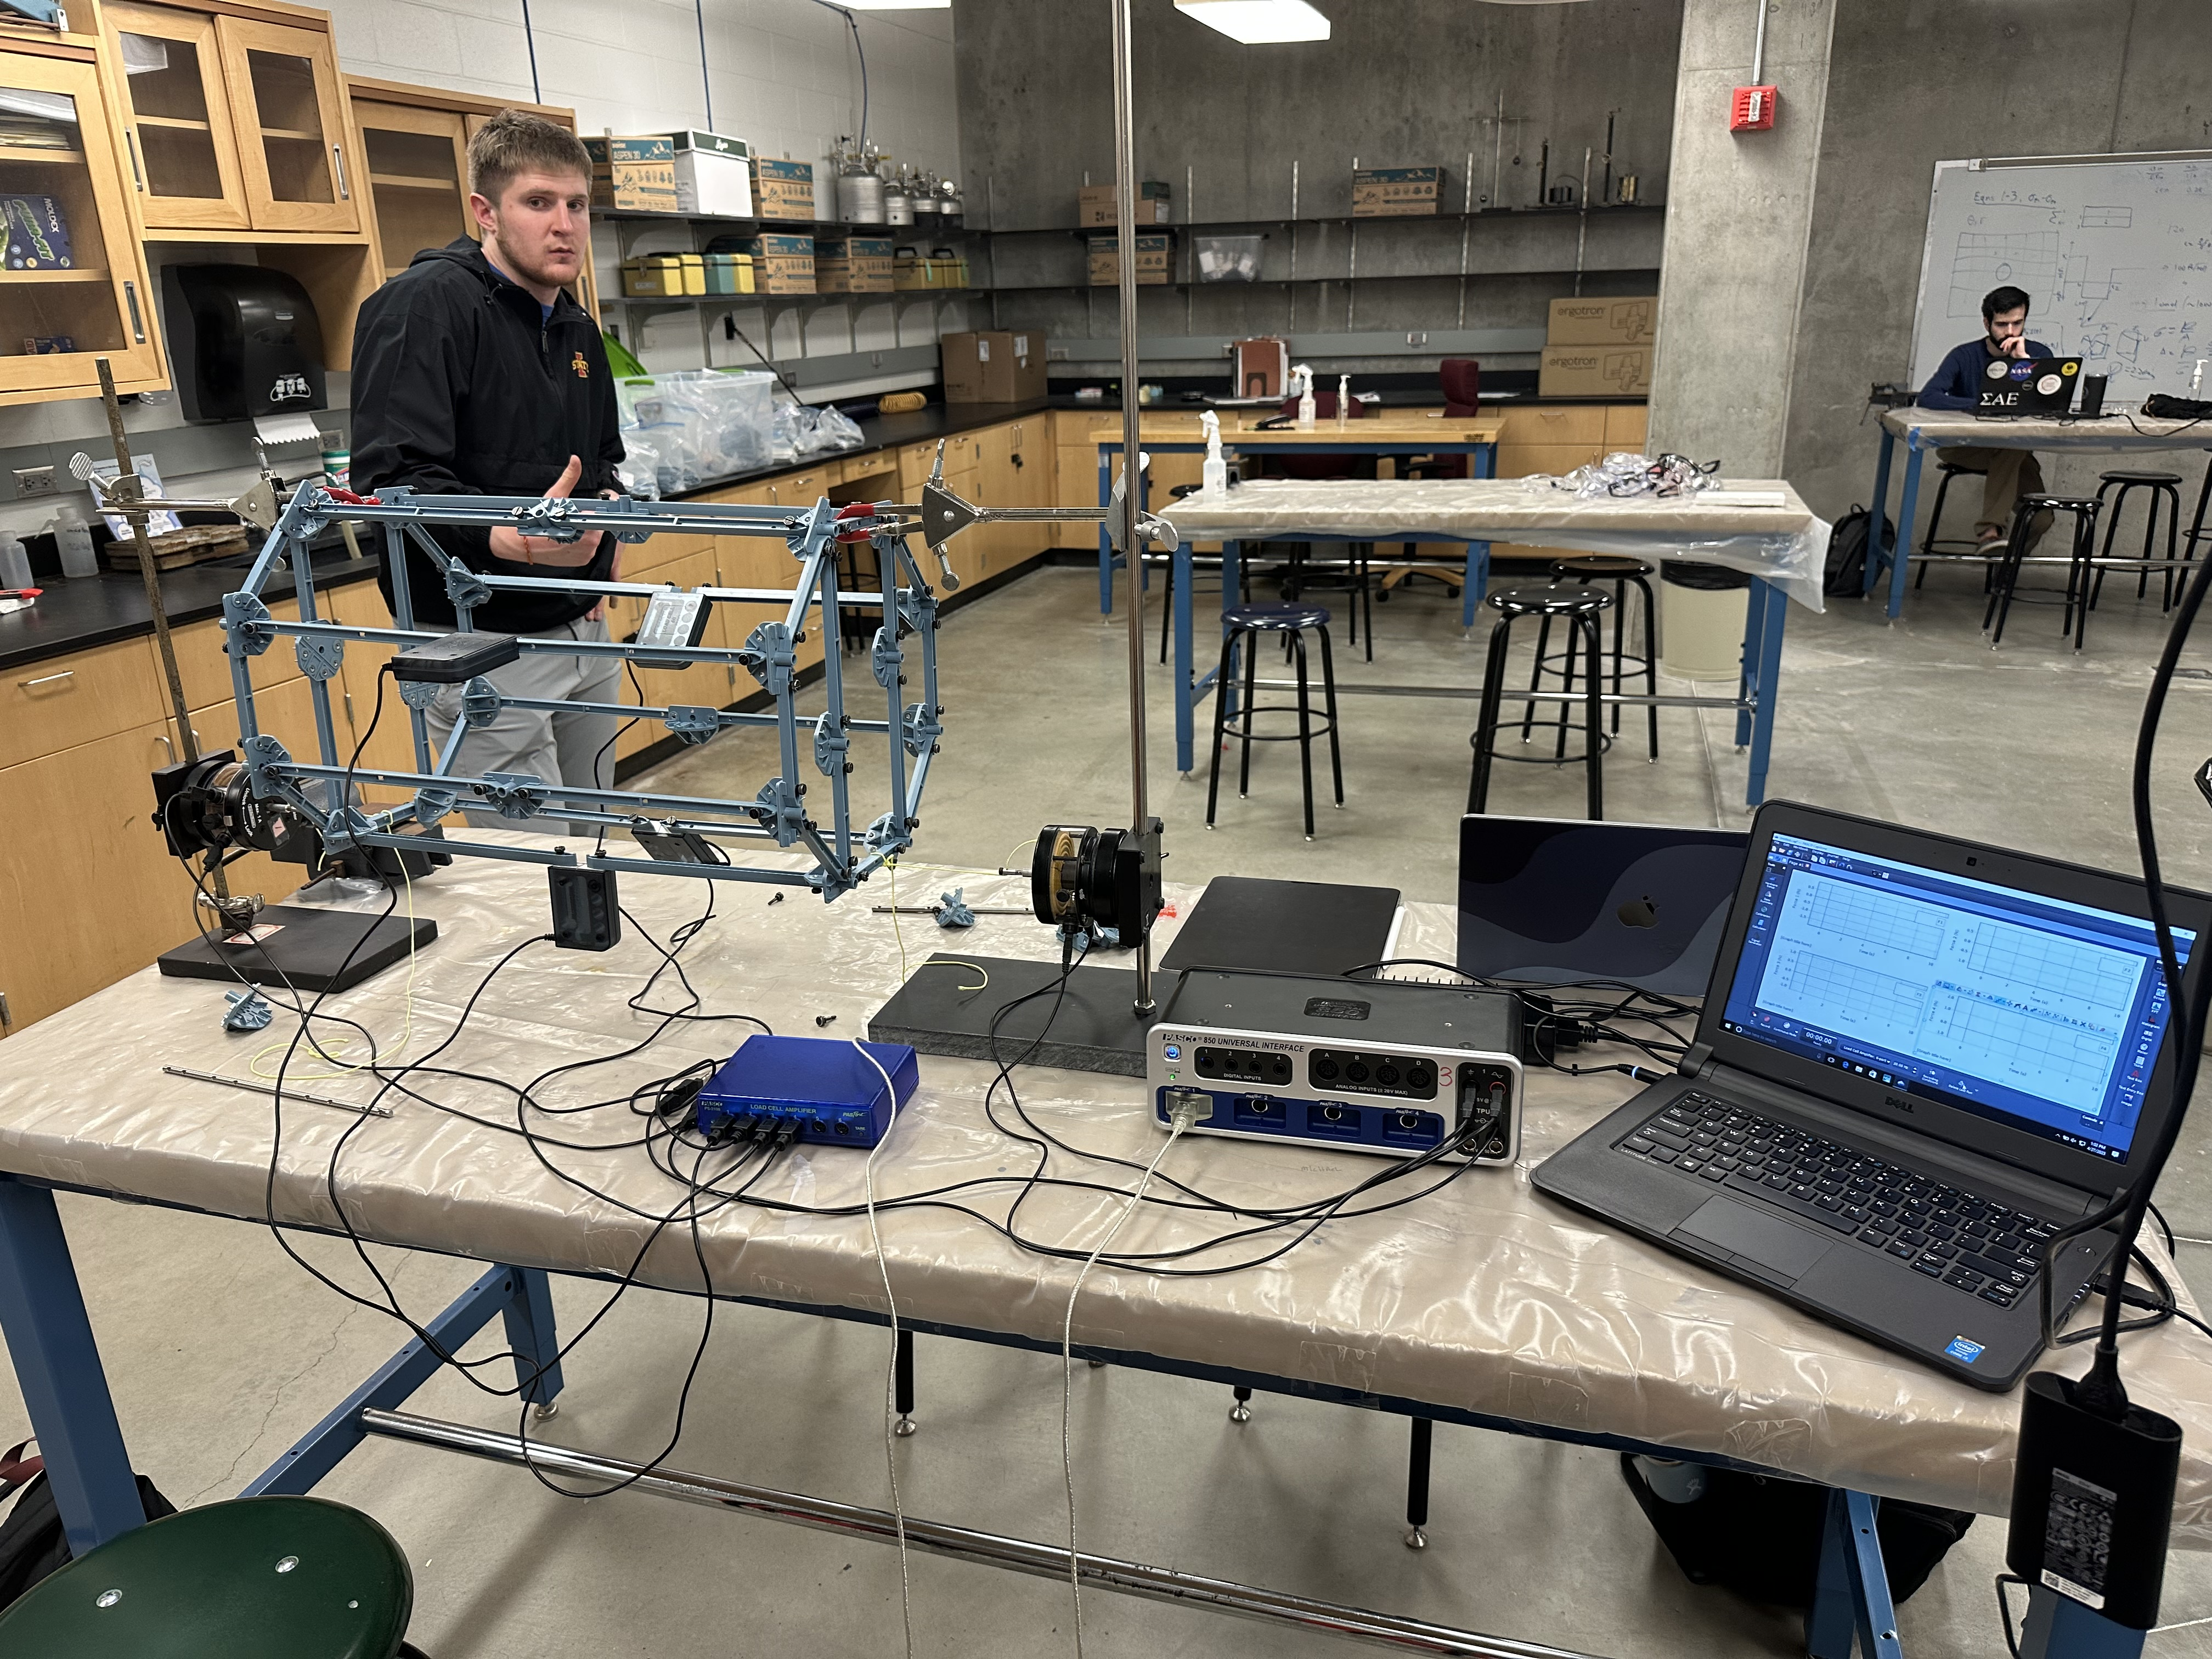
\includegraphics[width=4in]{images/IMG_1320}
	\caption{An image of the entire test \num {1} configuration.}
	\label{fig:test1_app_9}
\end{figure}

\begin{figure}[htbp]
	\centering
	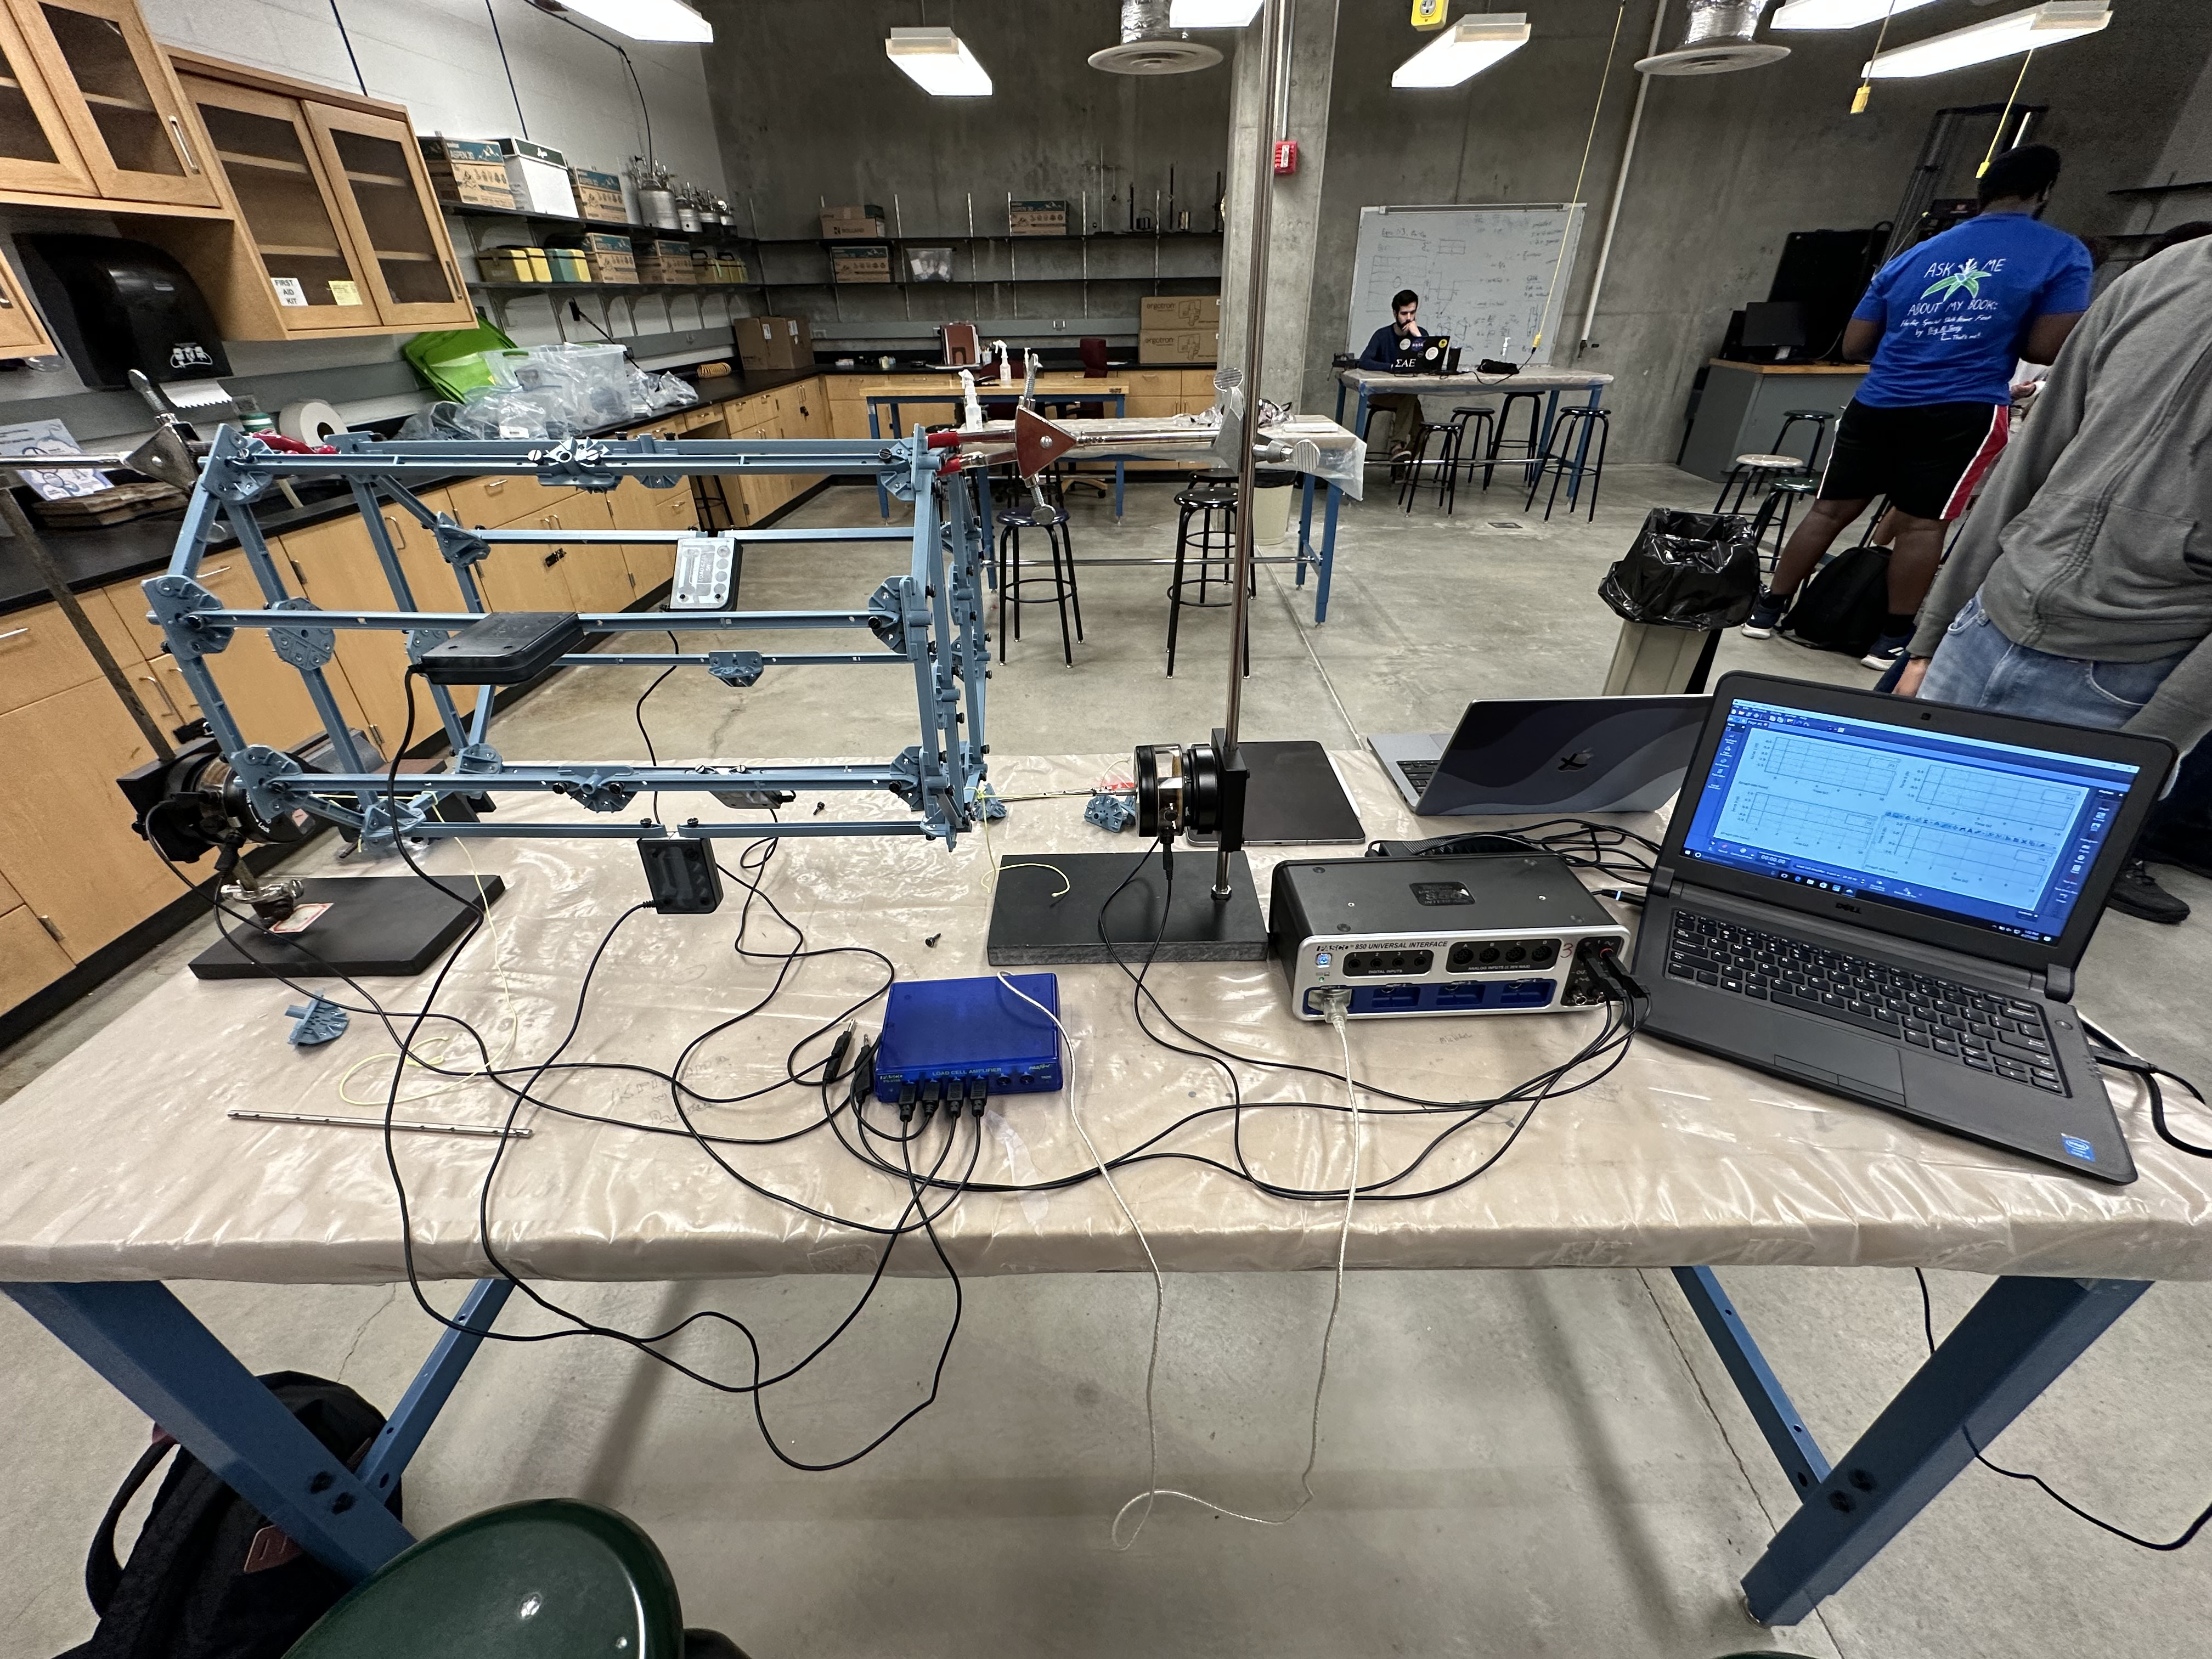
\includegraphics[width=4in]{images/IMG_1321}
	\caption{An image of the entire test \num{1} configuration.}
	\label{fig:test1_app_10}
\end{figure}

\begin{figure}[htbp]
	\centering
	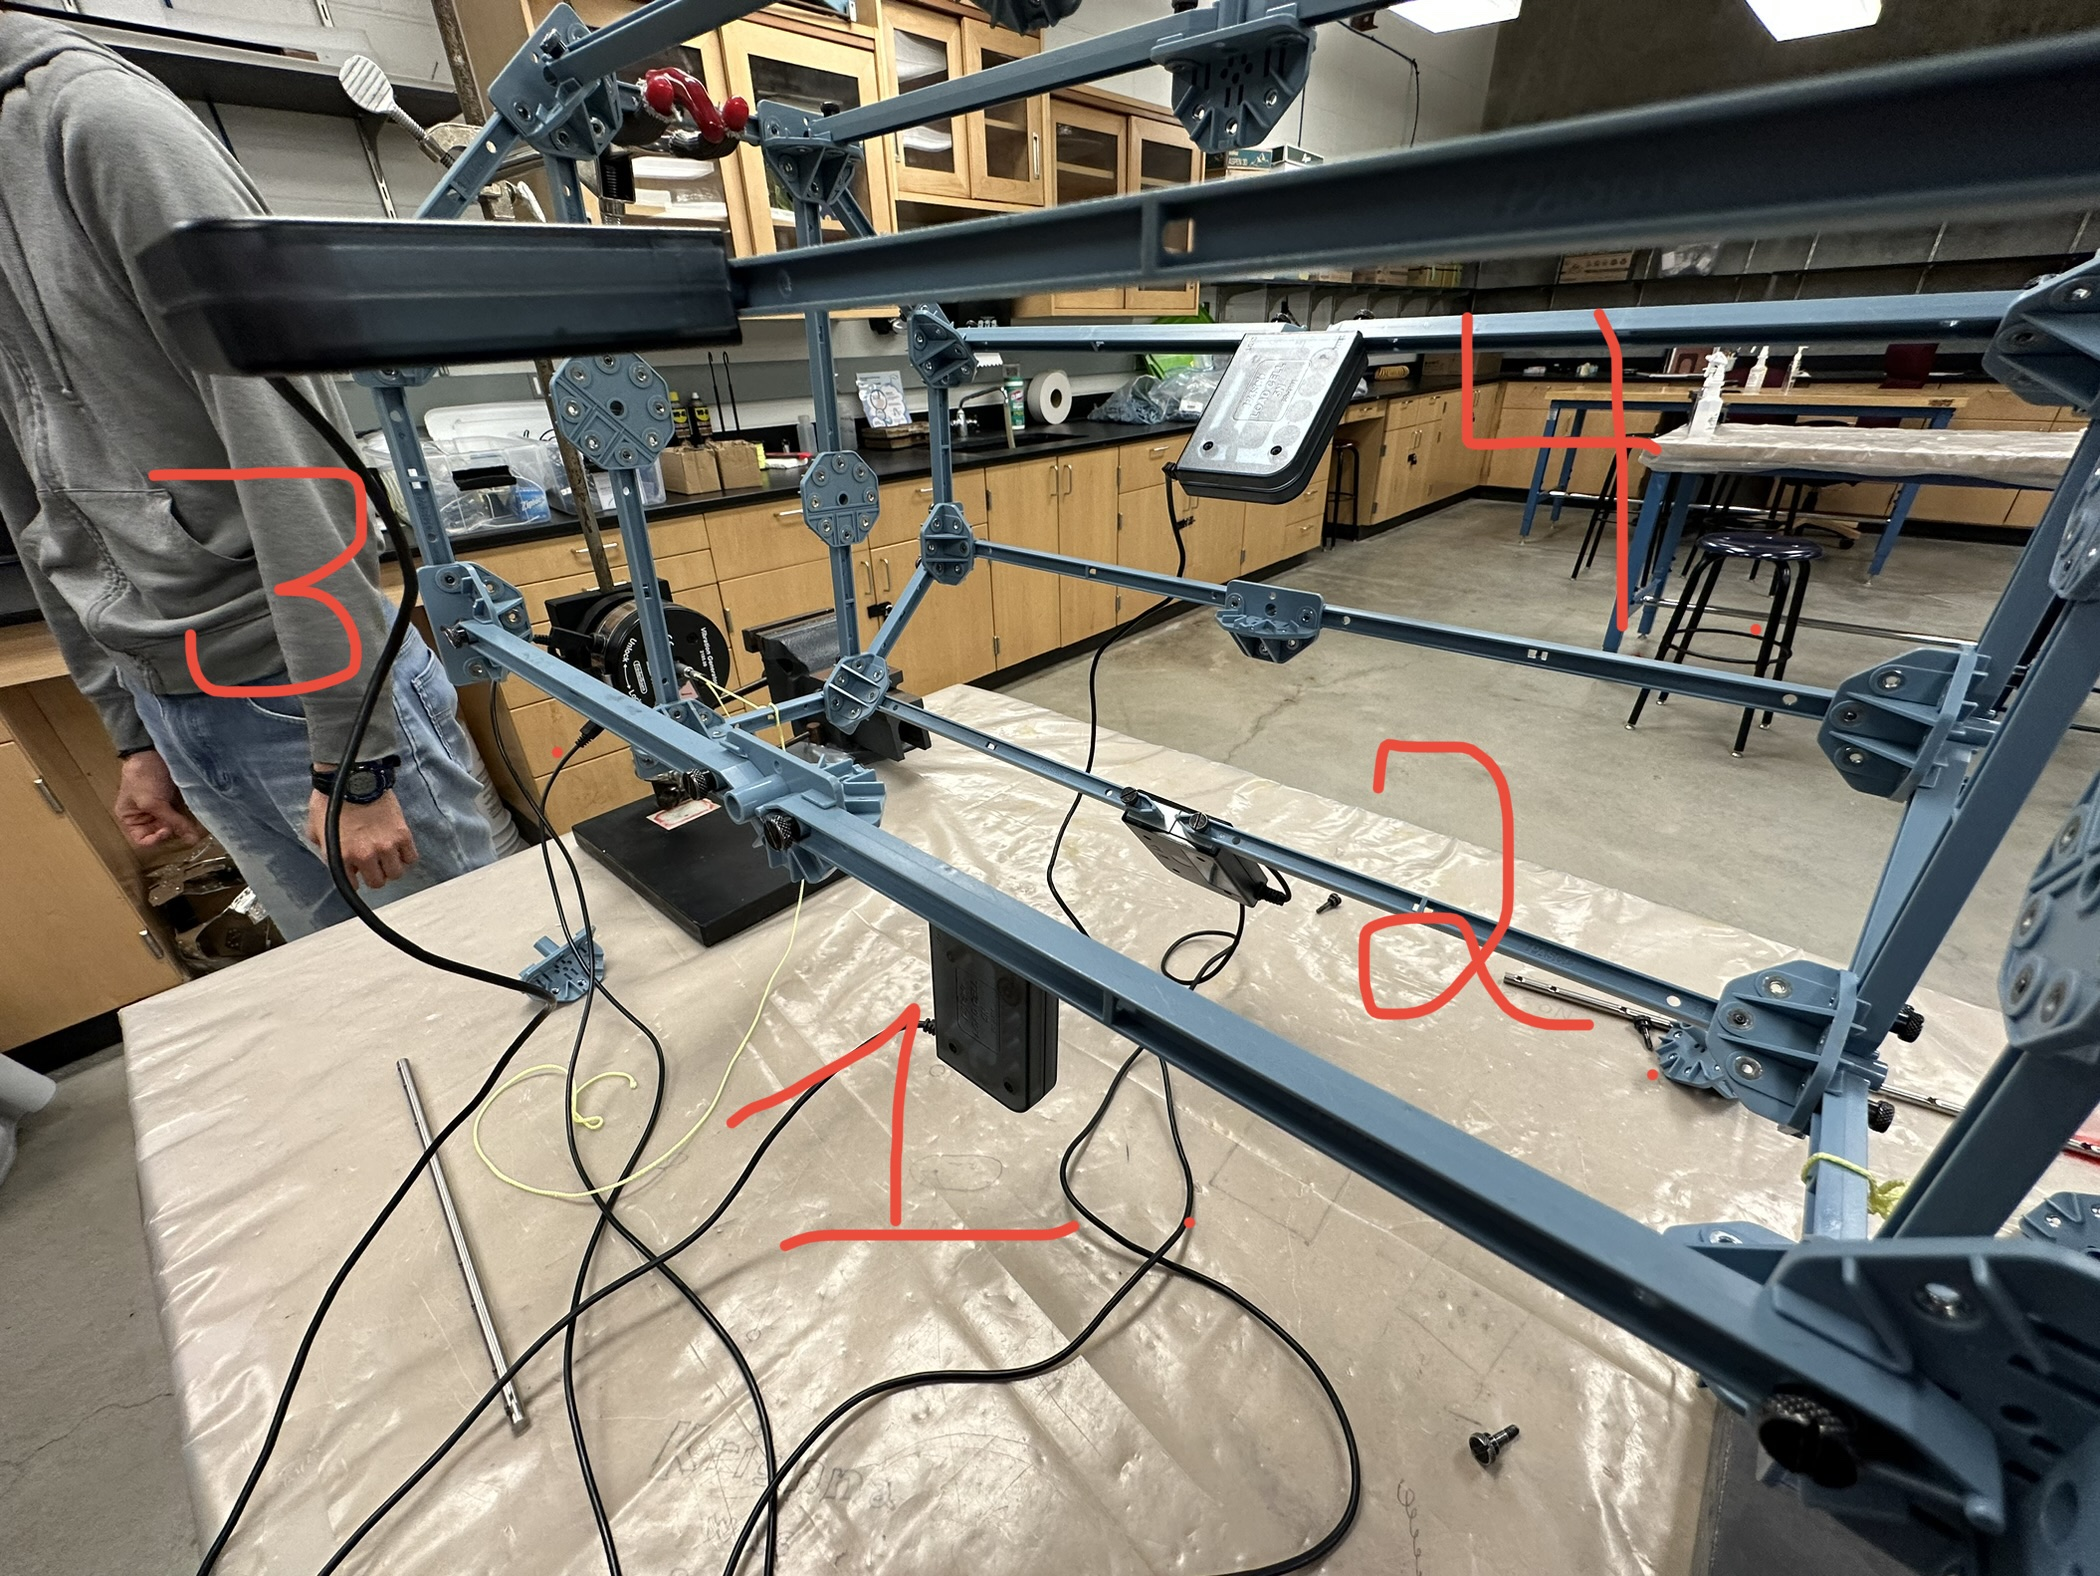
\includegraphics[width=4in]{images/IMG_1322}
	\caption{A close-up image with notations denoting which load cells correspond to which data points.}
	\label{fig:test1_app_11}
\end{figure}

The load cell calibration apparatus is shown in Figure \ref{fig:load_cell_calibration}

\begin{figure}[htbp]
	\centering
	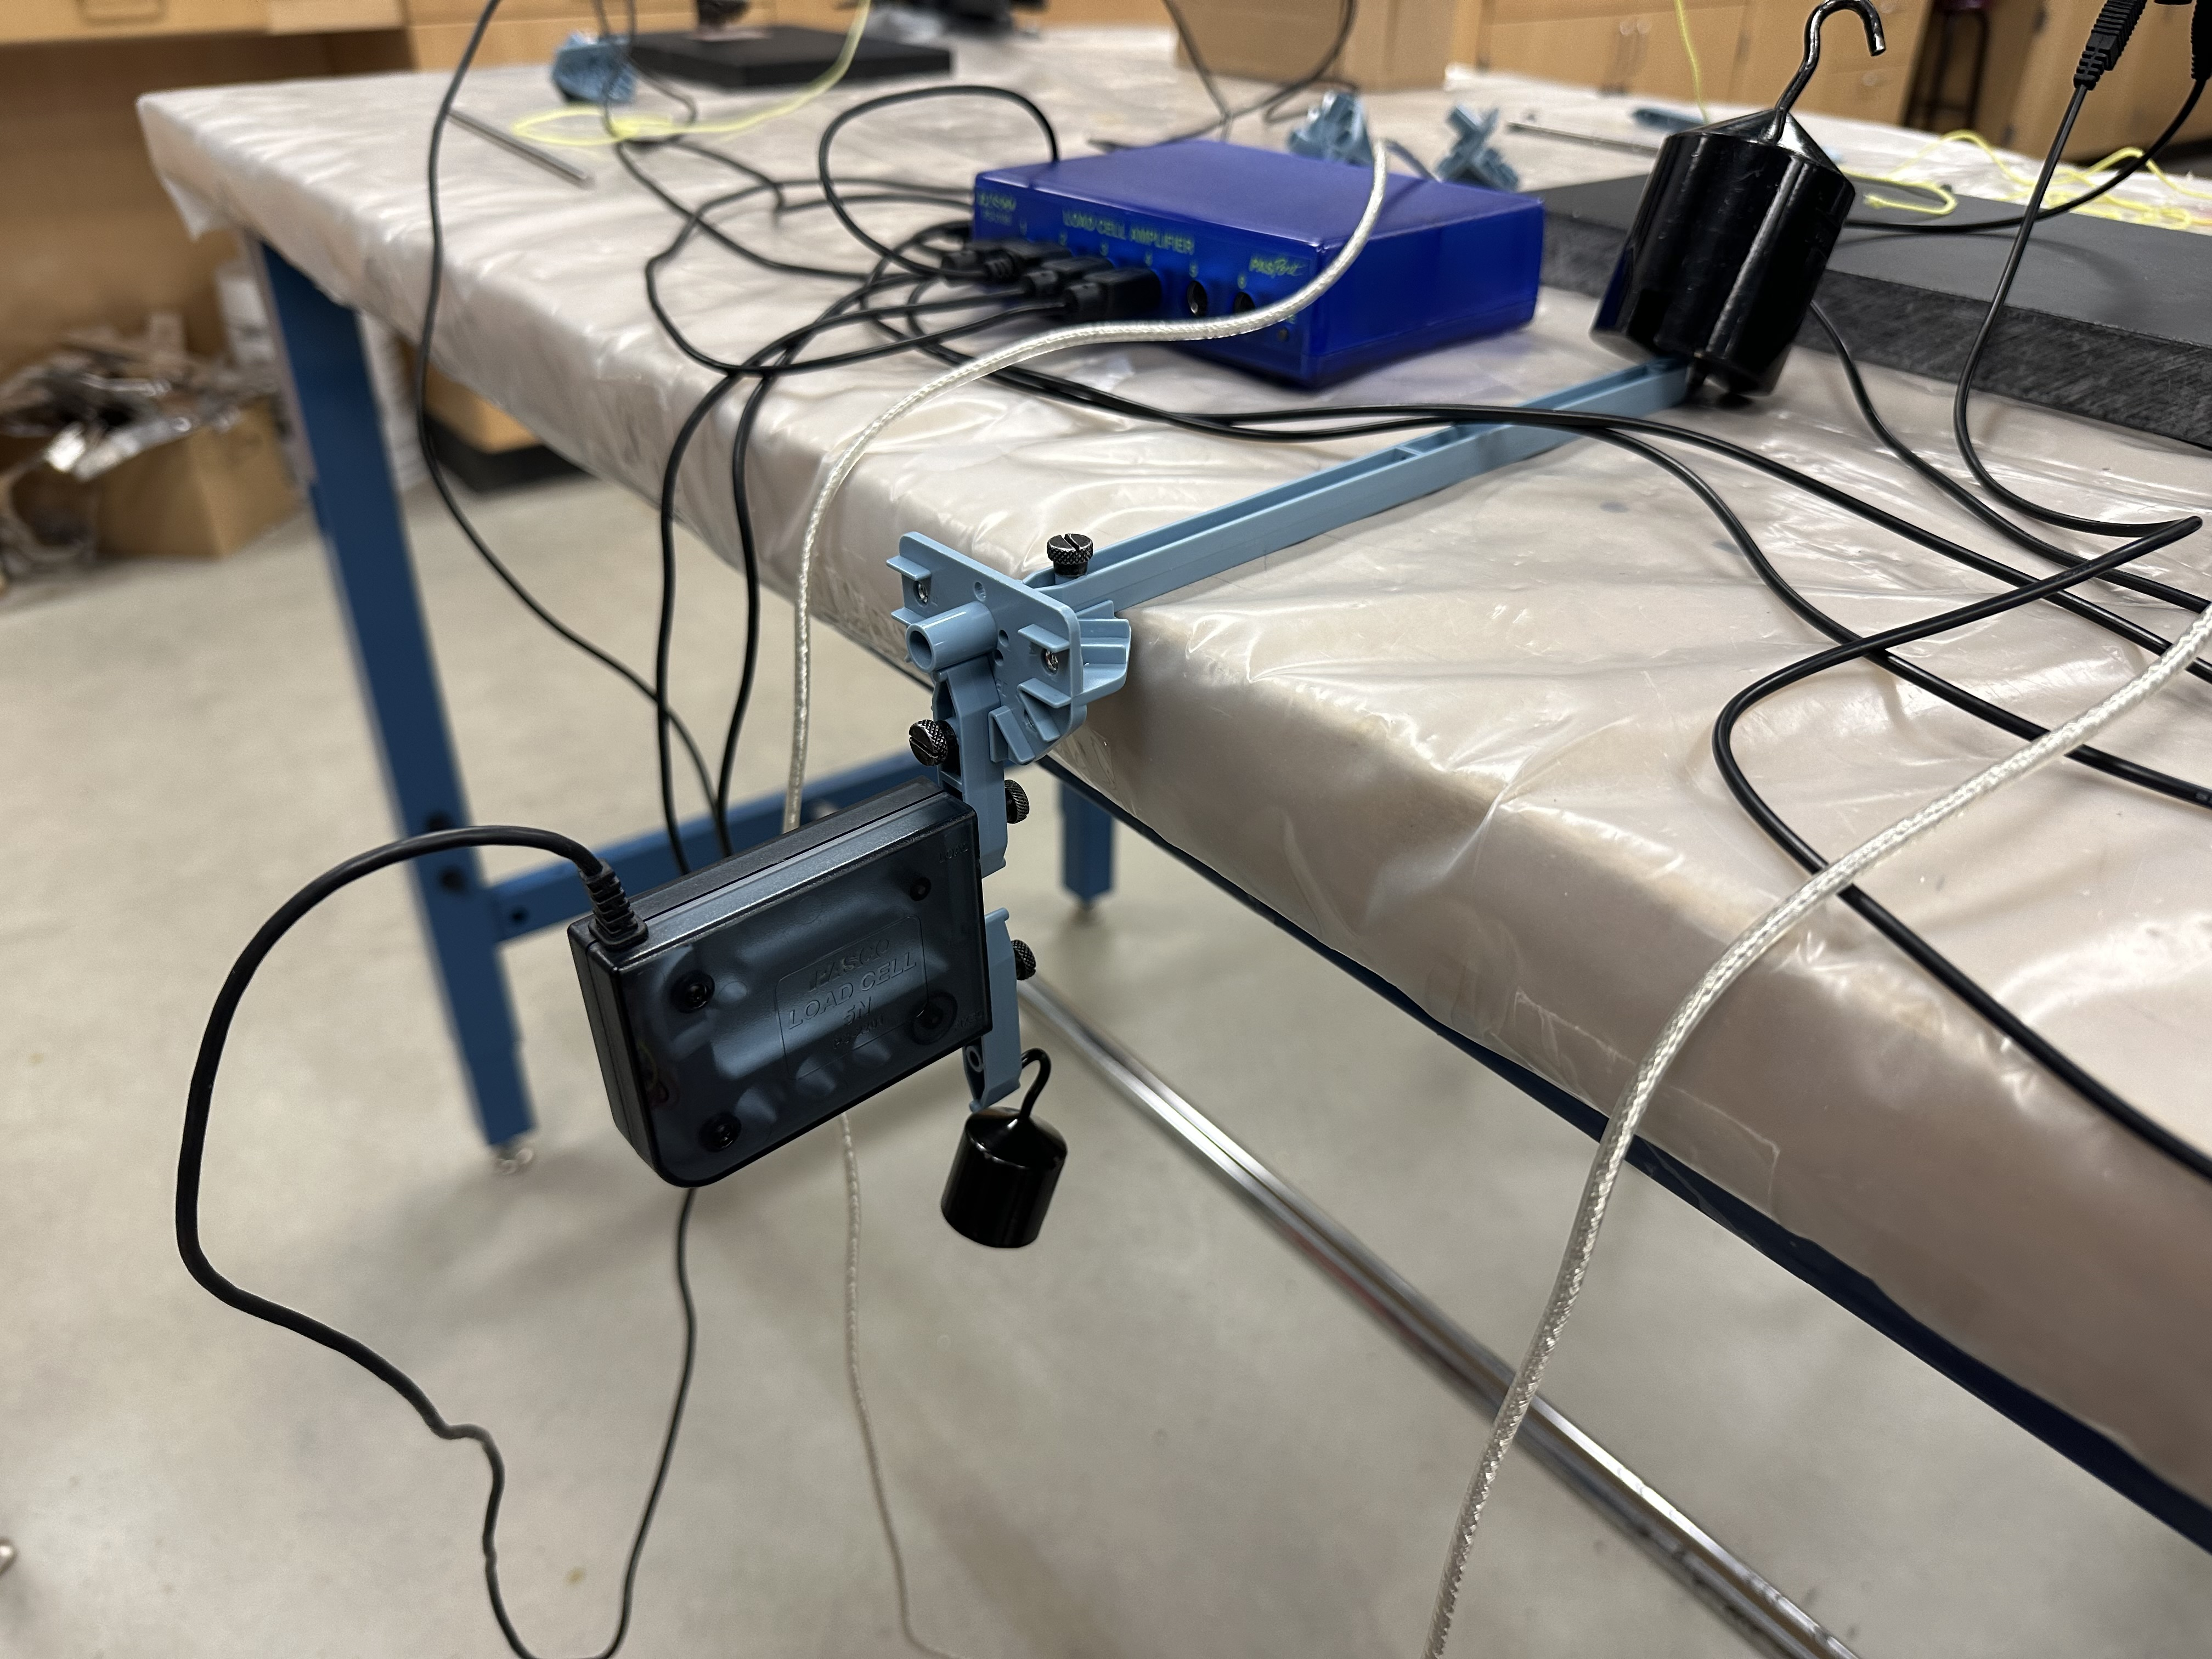
\includegraphics[width=4in]{images/IMG_1323}
	\caption{A close-up image of the load cell calibration apparatus with a \qty{50}{\gram} mass applied.}
	\label{fig:load_cell_calibration}
\end{figure}

The test \num{2} apparatus is shown in Figures \ref{fig:test2_app_1}--\ref{fig:test2_app_3}.

\begin{figure}[htbp]
	\centering
	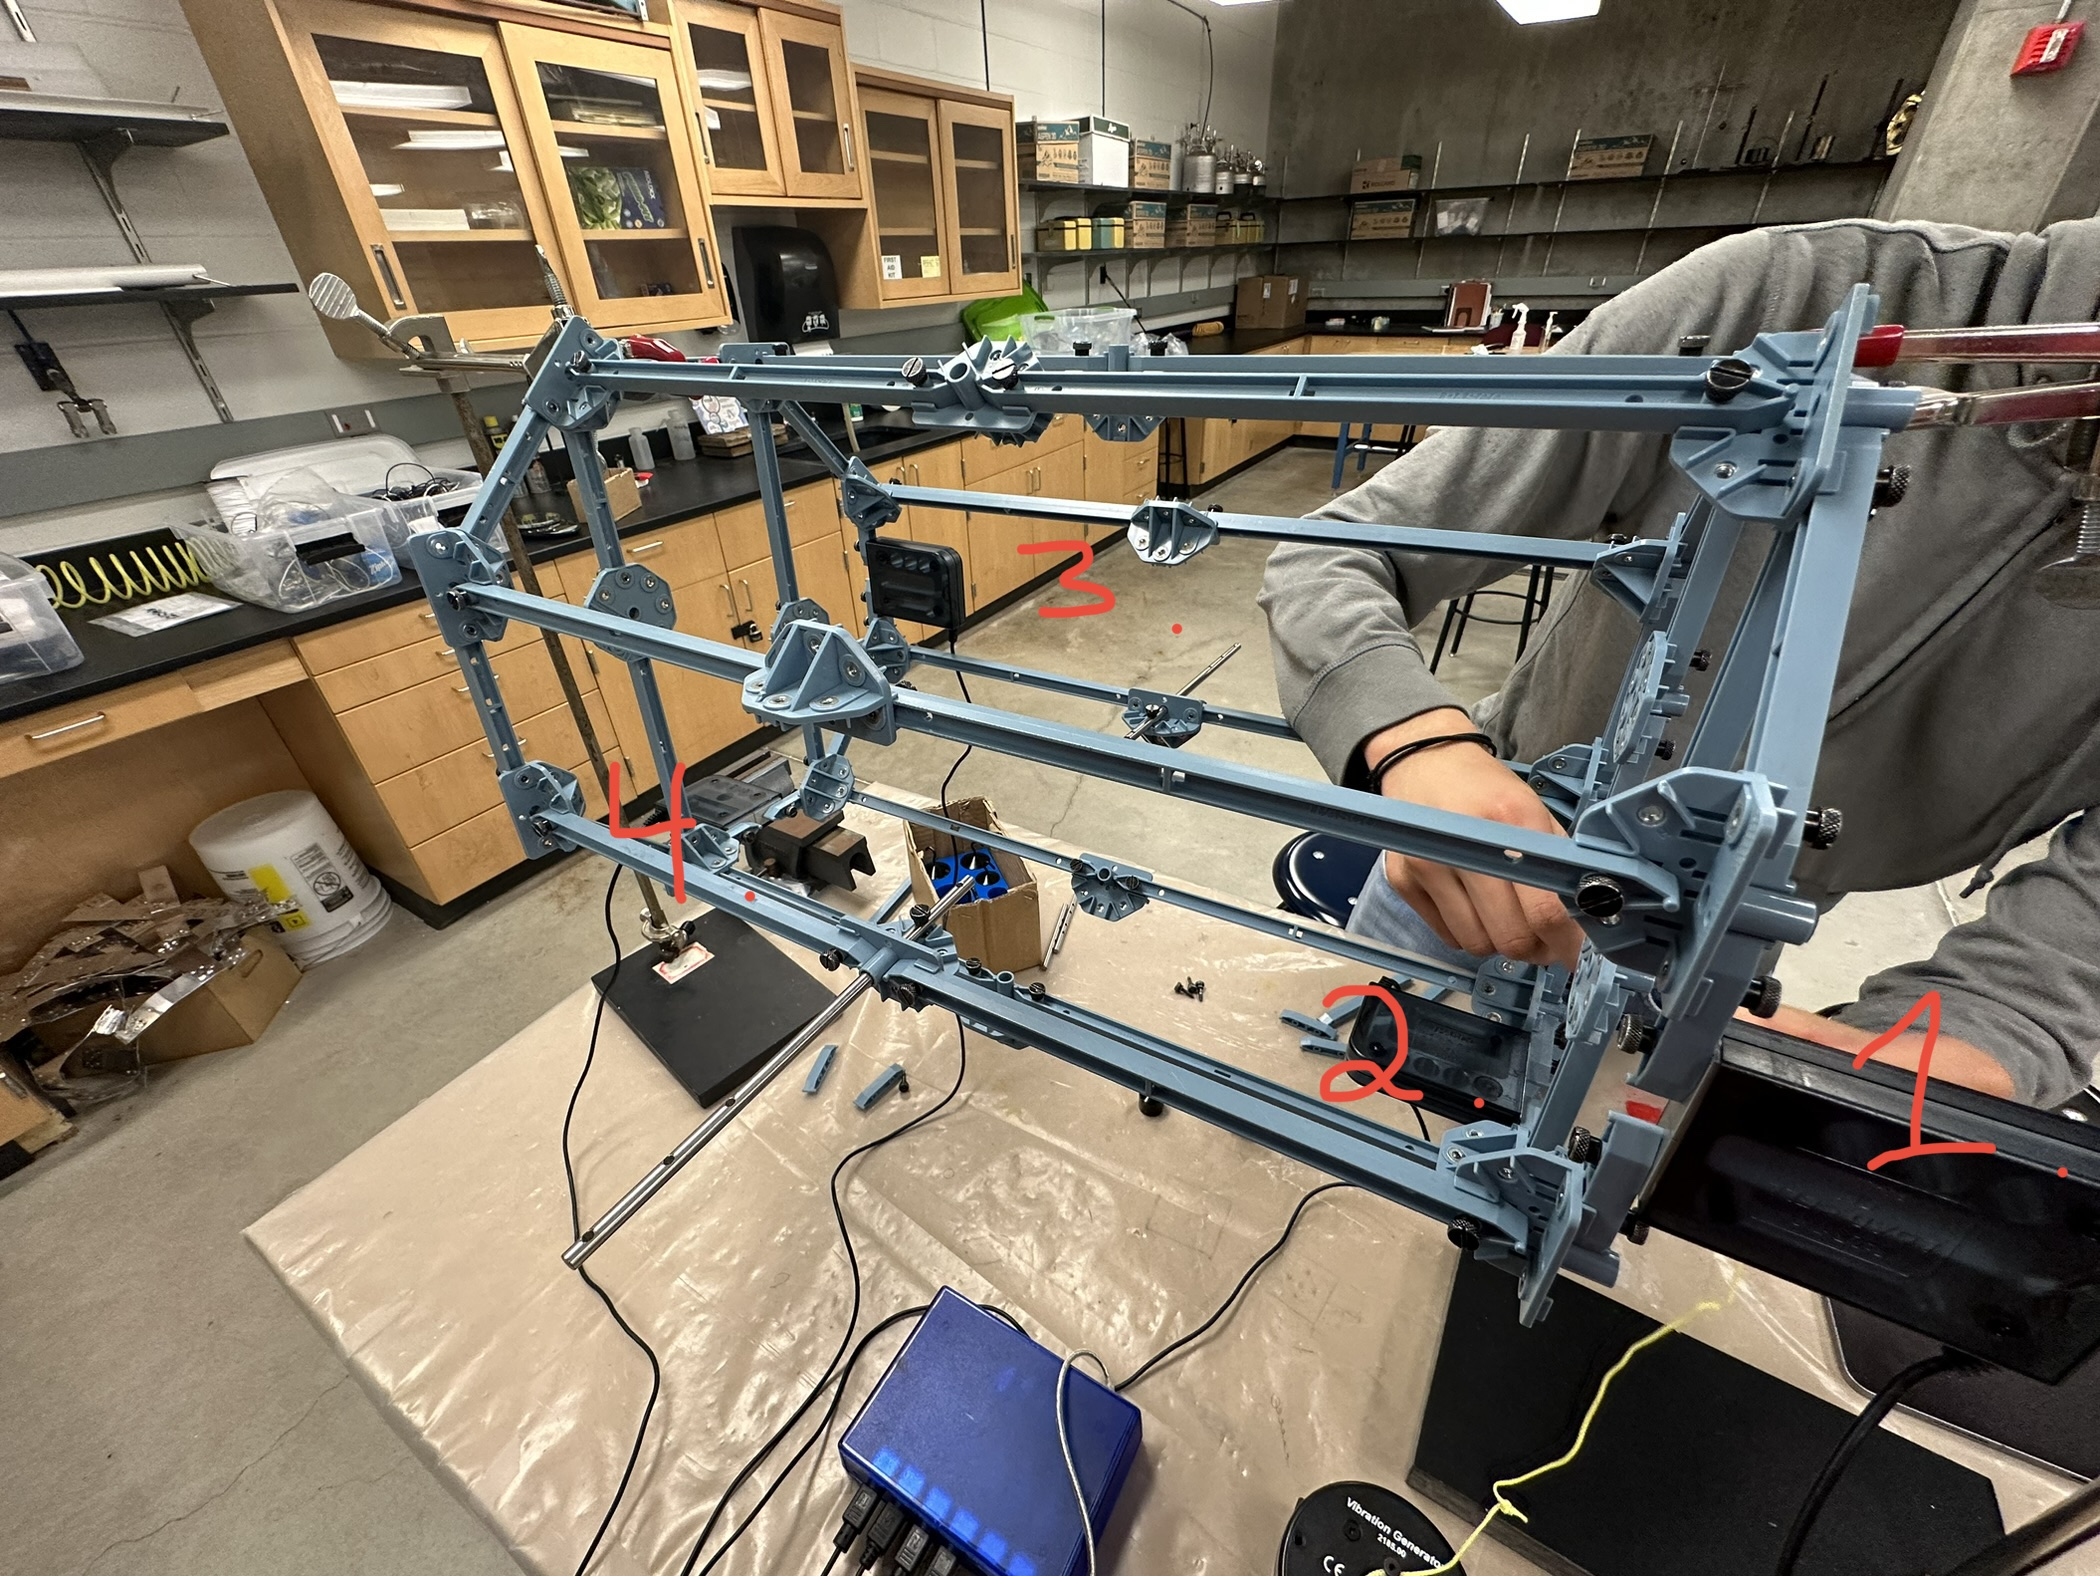
\includegraphics[width=4in]{images/IMG_1326}
	\caption{An image with notations denoting the position of the load cells and which load cells corresponds to which data points for test configuration \num{2}.}
	\label{fig:test2_app_1}
\end{figure}

\begin{figure}[htbp]
	\centering
	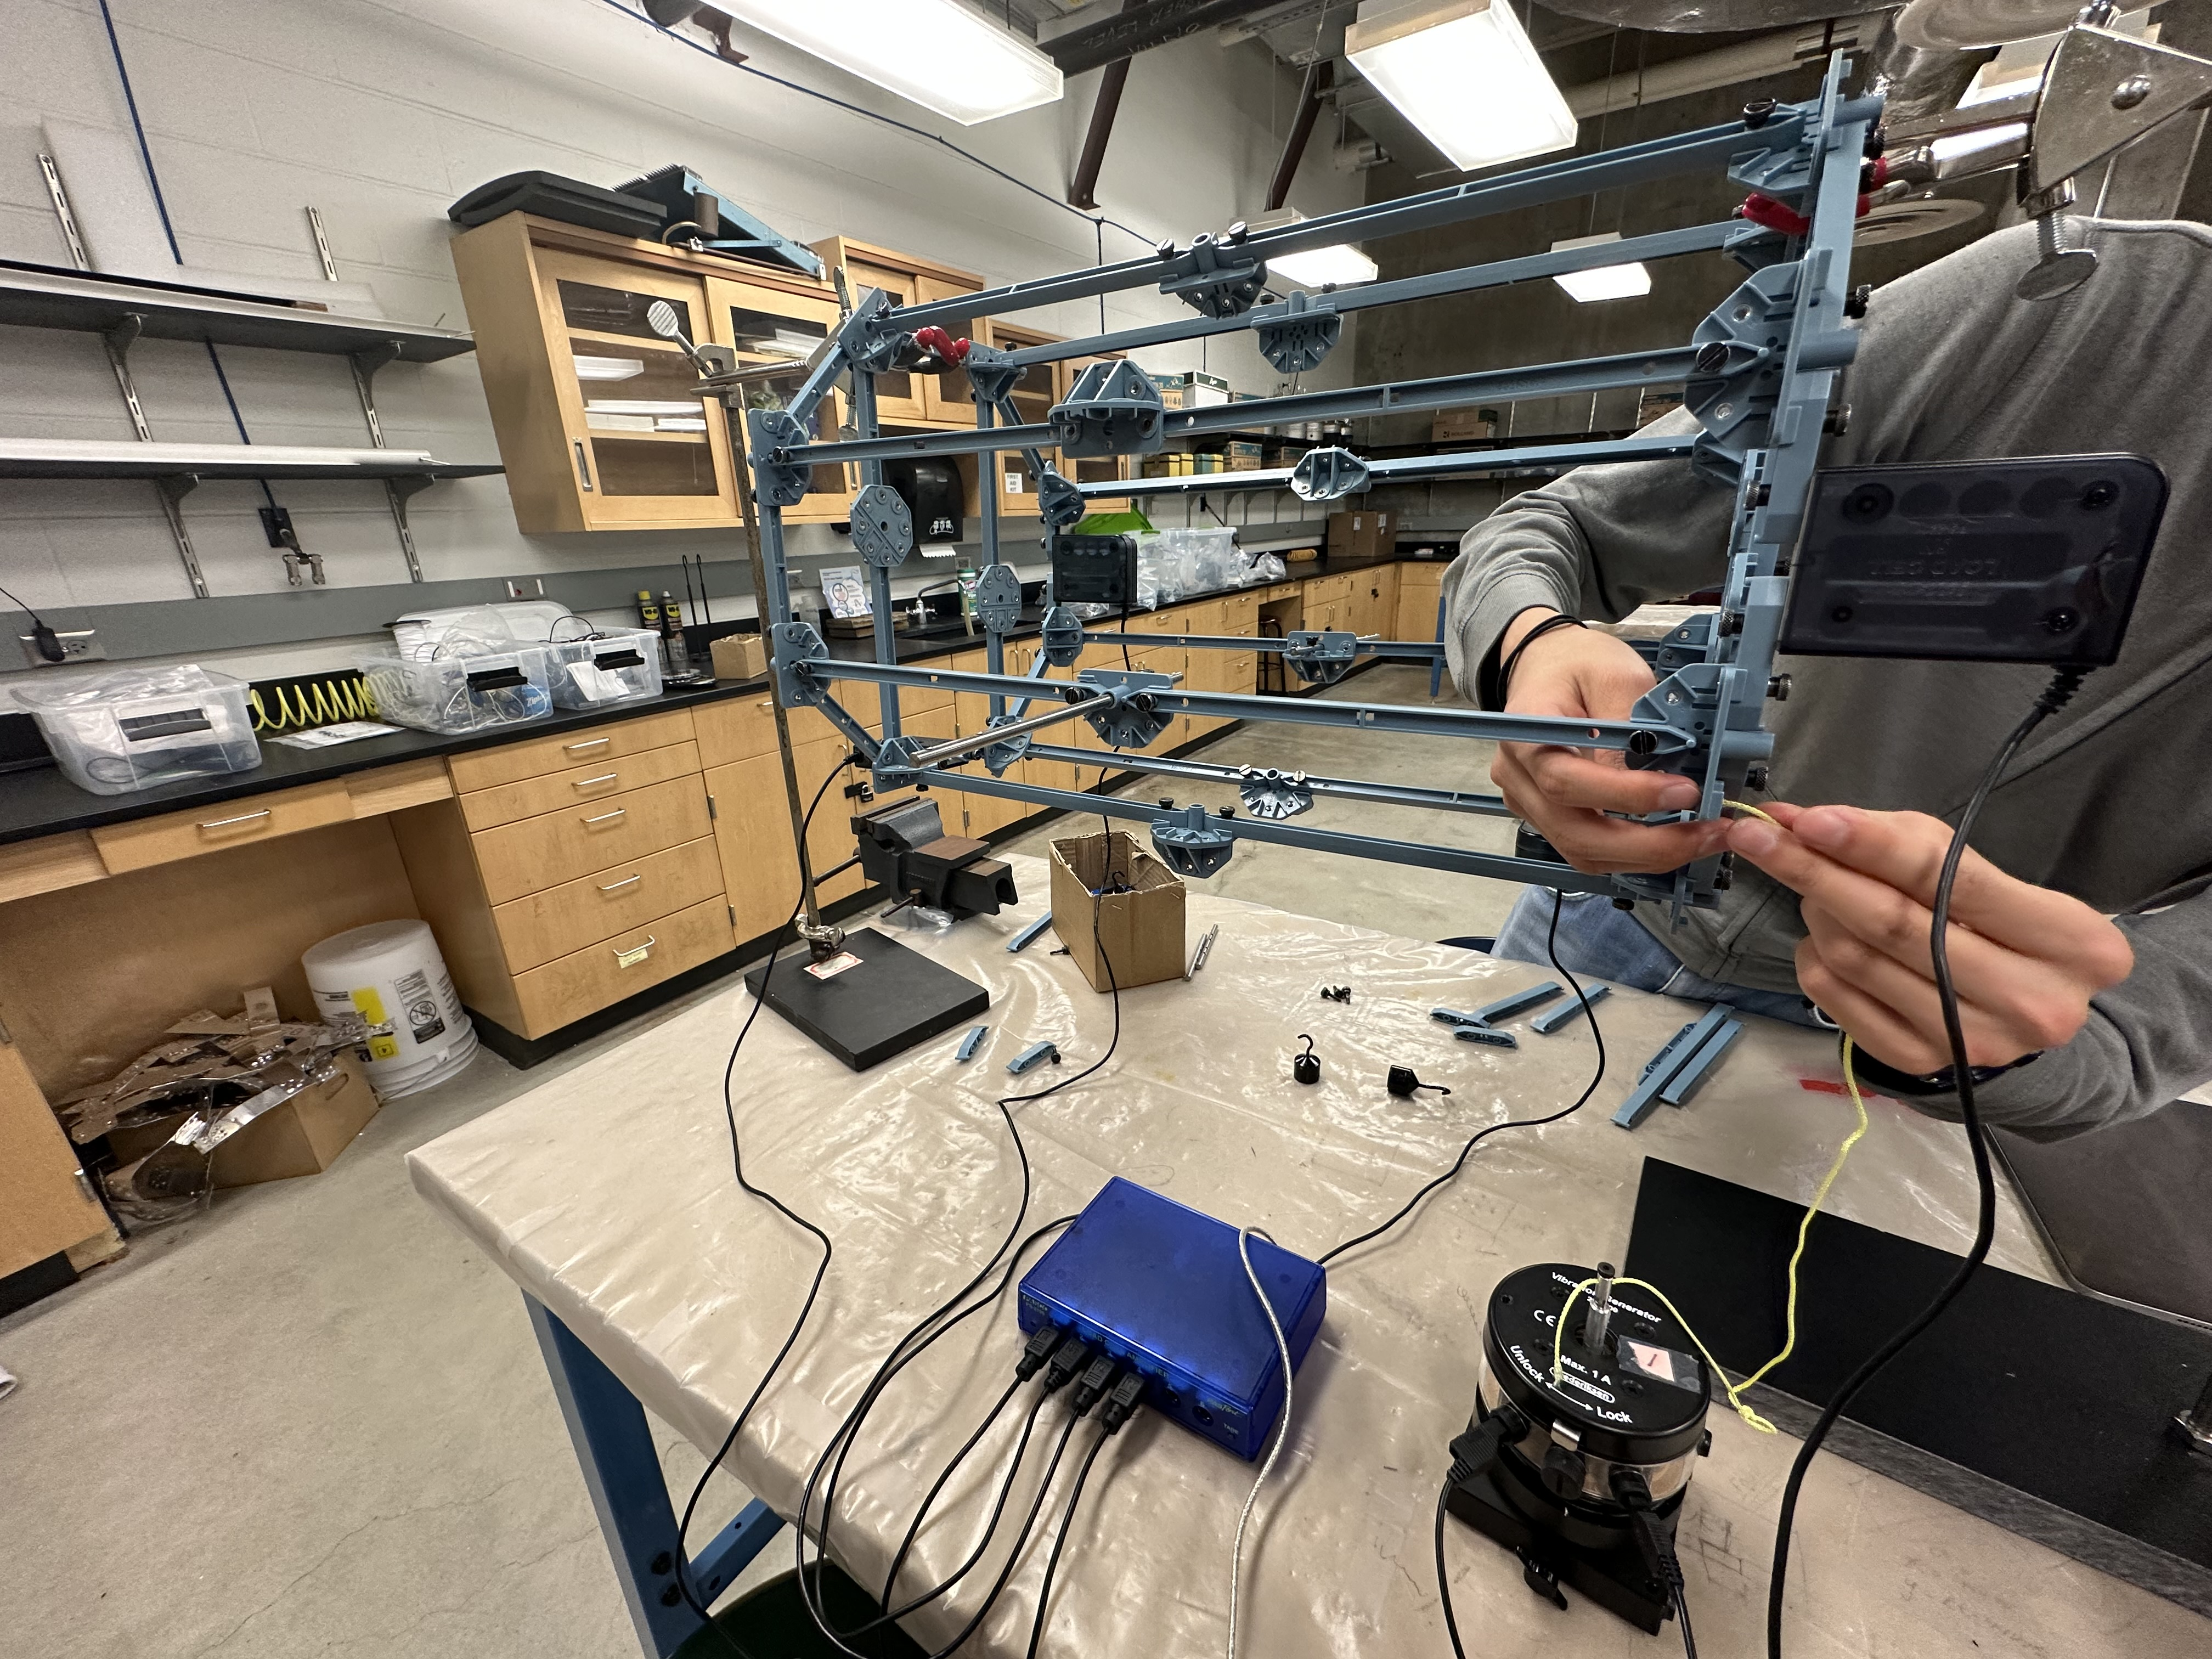
\includegraphics[width=4in]{images/IMG_1327}
	\caption{An image of the test \num{2} configuration. Note the position of the single wave driver versus the two wave drivers in test configuration \num{1}.}
	\label{fig:test2_app_2}
\end{figure}

\begin{figure}[htbp]
	\centering
	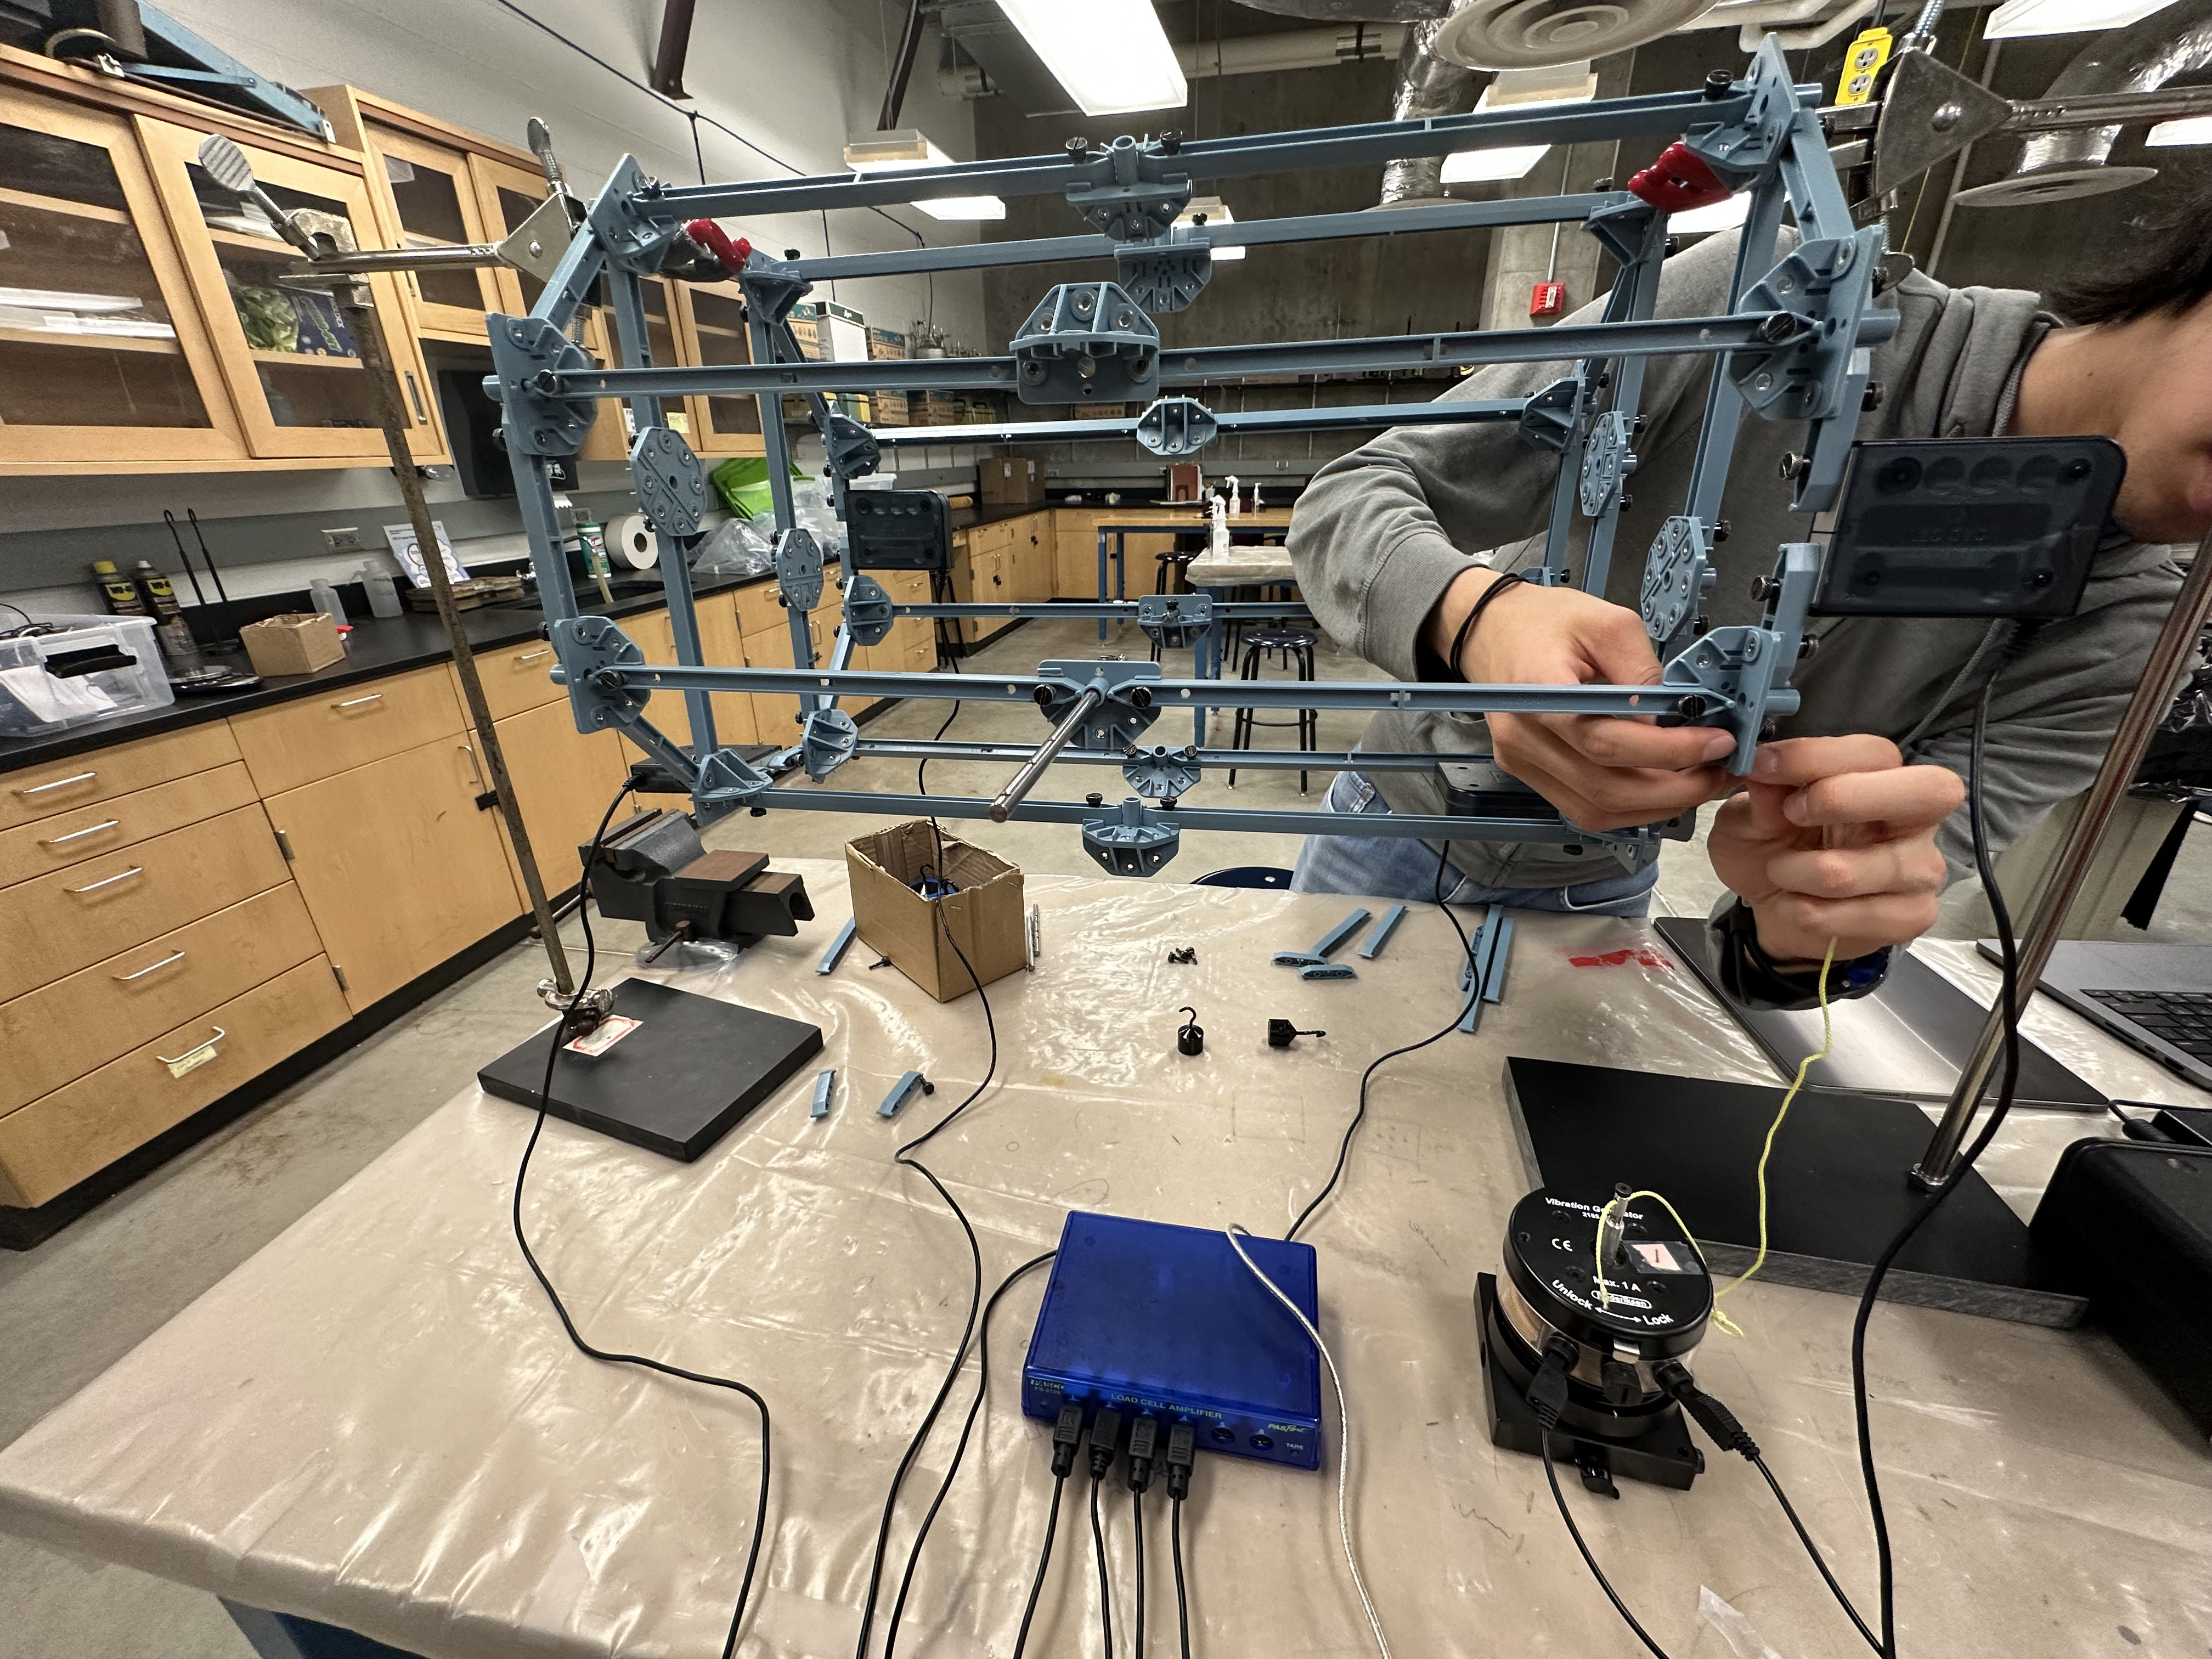
\includegraphics[width=4in]{images/IMG_1329}
	\caption{Another overall image of the test \num{2} configuration.}
	\label{fig:test2_app_3}
\end{figure}

\section{Procedures} \label{procedures}
% TODO: Revise
\subsection{Building} \label{building}
Build two octagons with size \num{3} bars of PASCO tool kit and hinges that connects each bar. When building two sections, make sure that all hinge used for an octagon connects with same direction, and its direction for joining bar is opposite to the other section. Set two vertical bars on each section for reinforce. Join two built octagons with two size \num{5} bars joined using a half circle connection and fasten the end of long bar on each vertex of each octagon. Fasten both the end of the fuselage model by two clamps of steel stand. Ensure that the fuselage model is horizontal to the ground. Four load cells that is connected computer through a hub is set on the fuselage model by using size \num{1} and \num{2} bars for connecting instead of size \num{5} bars. Make sure that which load cell is correspond to on the software by checking plug insertion. Load cell is numbered on the figure \ref{fig:test1_app_11}. Insert a wave driver through the pole of each steel stand horizontally to the bottom of testing structure; two wave drivers are required for horizontal vibration testing. Knot a fuselage model and wave driver tightly by a light string (Figures \ref{fig:test1_app_4} and \ref{fig:test1_app_5}). 

When test \num{2} is being conducted, change the construction of the fuselage model; move each place of load cell set into the suitable ones as shown in Figure \ref{fig:test2_app_1}.

\subsection{Calibration} \label{calibration}
We calibrated the load cells using the PASCO software and bars. This was done before each test to ensure the load cells were reading usable values. The calibration apparatus is shown in Figure \ref{fig:load_cell_calibration}.

Smaller mass is the mass which used for calibration, oppositely larger mass is used for fixing. A load cell that would be calibrated is connected by two size \num{1} bars, one of which smaller mass is applied on. Before hanging a small mass on the short bar, run a test the response from load cell by software, and then conduct a test just after suspending the mass on a short bar. Save both data about when applying a mass and when not applying a mass.  

\subsection{Software and Running} \label{software}
Open the PASCO software and set it up so four graphs are displayed, one for each load cell. All four graphs set the x-axis to time and the y-axis to force. The test needs to be configured with a stop condition that automatically stops the test after \qty{15}{\second}. Then set the sampling rate to \qty{20}{\hertz} and configure the signal generator as shown in Figure \ref{fig:signal_generator}.

\begin{figure}[htbp]
	\centering
	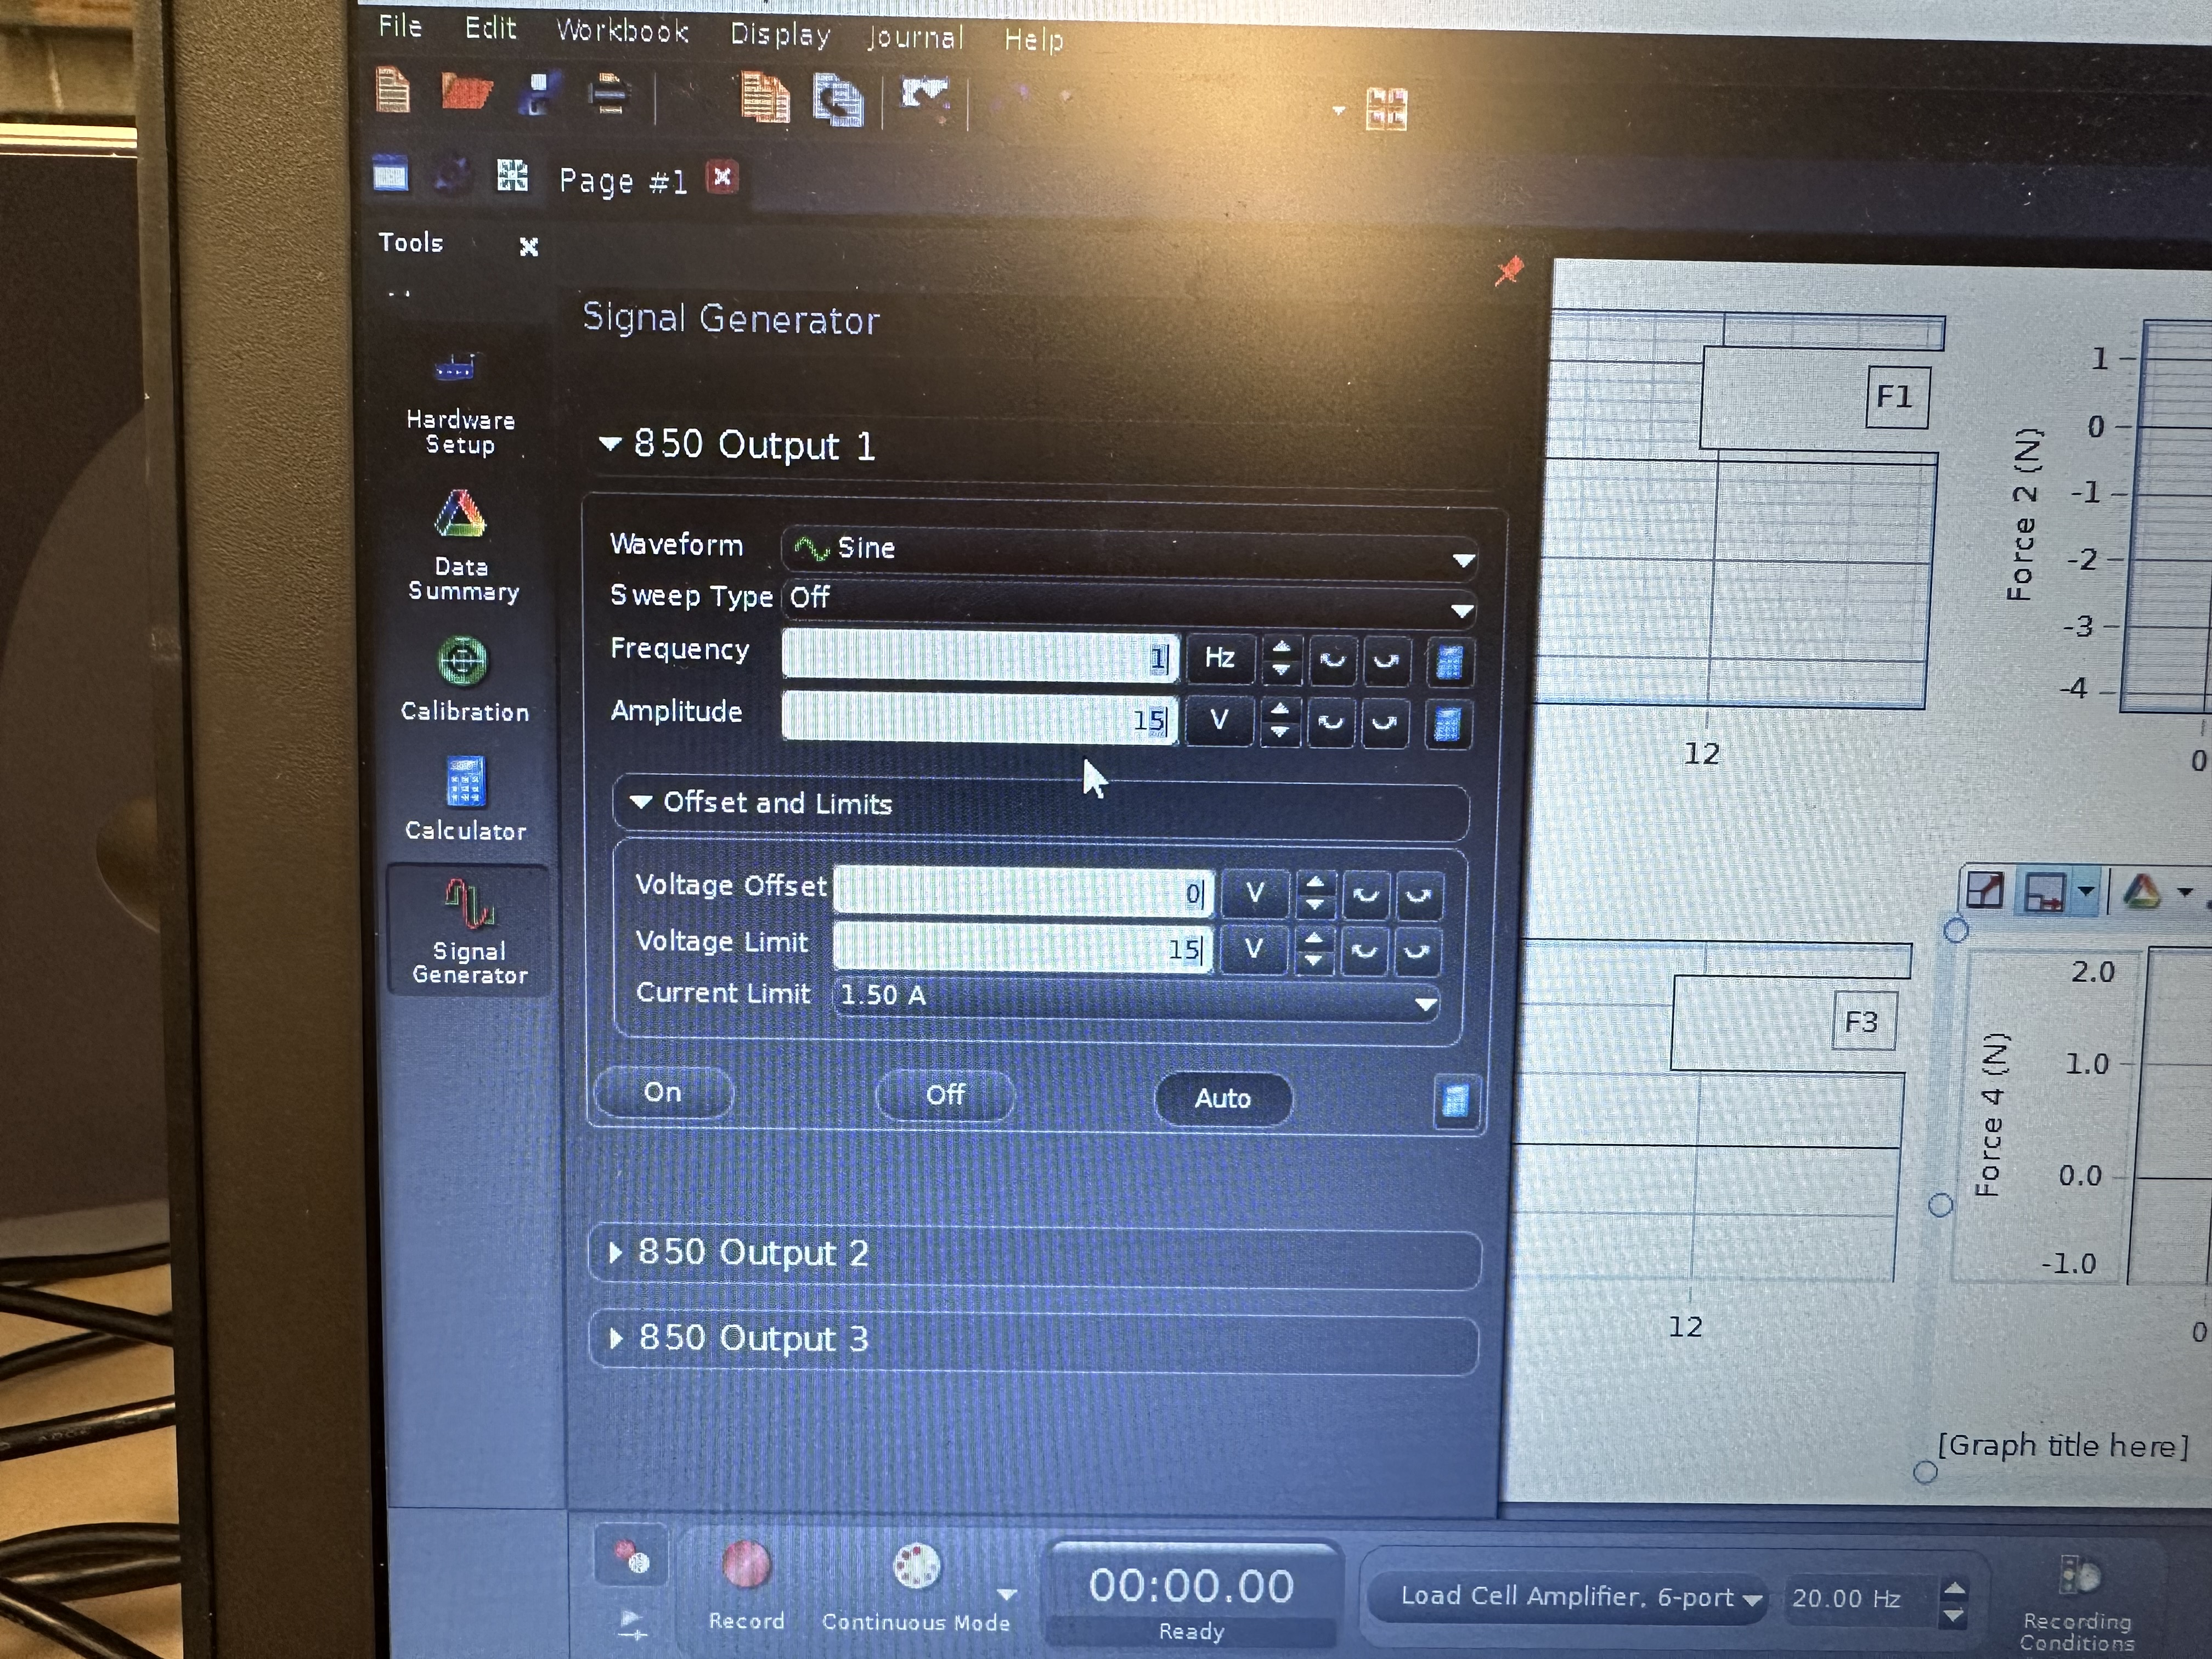
\includegraphics[width=4in]{images/IMG_1330}
	\caption{The software configuration of the signal generator.}
	\label{fig:signal_generator}
\end{figure}

Each test has five rounds of testing that will be run in order of \qtylist{1;2;5;10;15}{\hertz}. Ensure that the strings tied to the system are taught and run the first round of testing by clicking ``start.'' Once the test runs for the duration, export all the data using the ``export'' function and save it as a .txt file. Change the frequency of the wave driver to run the next test and ensure that the string is taught after each round of testing. The wave driver can pull too hard, causing the string to come loose.

\section{Data} \label{data}
The raw data for run \num{1} in tests \numlist{1;2} are shown in Figures \ref{fig:test1_run1} and \ref{fig:test2_run1}. Note the different average values for each load cell.

\begin{figure}[htbp]
	\centering
	\includesvg[width=4in]{images/graphs/force-vs-time-test-1-run-1}
	\caption{The raw force data from test \num{1} run \num{1}.}
	\label{fig:test1_run1}
\end{figure}

\begin{figure}[htbp]
	\centering
	\includesvg[width=4in]{images/graphs/force-vs-time-test-2-run-1}
	\caption{The raw force data from test \num{2} run \num{1}.}
	\label{fig:test2_run1}
\end{figure}

After subtracting out the different baselines for each load cell, the data can be plotted uniformly about the $x$-axis as shown in Figures \ref{fig:test1_run1_baseline_removed} and \ref{fig:test2_run1_baseline_removed}.

\begin{figure}[htbp]
	\centering
	\includesvg[width=4in]{images/graphs/force-vs-time-baseline-removed-test-1-run-1}
	\caption{The force data plotted uniformly about the $x$-axis from test \num{1} run \num{1}.}
	\label{fig:test1_run1_baseline_removed}
\end{figure}

\begin{figure}[htbp]
	\centering
	\includesvg[width=4in]{images/graphs/force-vs-time-baseline-removed-test-2-run-1}
	\caption{The force data plotted uniformly about the $x$-axis from test \num{2} run \num{1}.}
	\label{fig:test2_run1_baseline_removed}
\end{figure}

To account for minor fluctuations in the force measurements, we applied a simple rolling smoothing function with a window of \num{3} data points to clean the data. An example of un-smoothed data is shown in Figure \ref{fig:test1_run1_baseline_removed_5_to_6} and the smoothed grpah is shown in Figure \ref{fig:test1_run1_baseline_removed_smoothed_5_to_6}.

\begin{figure}[htbp]
	\centering
	\includesvg[width=4in]{images/graphs/force-vs-time-baseline-removed-5-s-to-6-s-test-1-run-1}
	\caption{The force data plotted uniformly about the $x$-axis from test \num{1} run \num{1}. Only \qtyrange{5}{6}{\second} are shown.}
	\label{fig:test1_run1_baseline_removed_5_to_6}
\end{figure}

\begin{figure}[htbp]
	\centering
	\includesvg[width=4in]{images/graphs/force-vs-time-smoothed-baseline-removed-5-s-to-6-s-test-1-run-1}
	\caption{The smoothed force data plotted uniformly about the $x$-axis from test \num{1} run \num{1}. Only \qtyrange{5}{6}{\second} are shown.}
	\label{fig:test1_run1_baseline_removed_smoothed_5_to_6}
\end{figure}

After applying smoothing and baseline removal, the results of test \num{1} runs \numrange{1}{5} are shown in Figures \ref{fig:test1_run1_results}--\ref{fig:test1_run5_results} and the results of test \num{2} runs \numrange{1}{5} are shown in Figures \ref{fig:test2_run1_results}--\ref{fig:test2_run5_results}. Only \qtyrange{5}{6}{\second} are shown for clarity. All graphs are shown in the appendix.

\begin{figure}[htbp]
	\centering
	\includesvg[width=3.8in]{images/graphs/force-vs-time-smoothed-baseline-removed-5-s-to-6-s-test-1-run-1}
	\caption{The smoothed force data plotted uniformly about the $x$-axis from test \num{1} run \num{1}. Only \qtyrange{5}{6}{\second} are shown.}
	\label{fig:test1_run1_results}
\end{figure}

\begin{figure}[htbp]
	\centering
	\includesvg[width=3.8in]{images/graphs/force-vs-time-smoothed-baseline-removed-5-s-to-6-s-test-1-run-2}
	\caption{The smoothed force data plotted uniformly about the $x$-axis from test \num{1} run \num{2}. Only \qtyrange{5}{6}{\second} are shown.}
	\label{fig:test1_run2_results}
\end{figure}

\begin{figure}[htbp]
	\centering
	\includesvg[width=3.8in]{images/graphs/force-vs-time-smoothed-baseline-removed-5-s-to-6-s-test-1-run-3}
	\caption{The smoothed force data plotted uniformly about the $x$-axis from test \num{1} run \num{3}. Only \qtyrange{5}{6}{\second} are shown.}
	\label{fig:test1_run3_results}
\end{figure}

\begin{figure}[htbp]
	\centering
	\includesvg[width=3.8in]{images/graphs/force-vs-time-smoothed-baseline-removed-5-s-to-6-s-test-1-run-4}
	\caption{The smoothed force data plotted uniformly about the $x$-axis from test \num{1} run \num{4}. Only \qtyrange{5}{6}{\second} are shown.}
	\label{fig:test1_run4_results}
\end{figure}

\begin{figure}[htbp]
	\centering
	\includesvg[width=3.8in]{images/graphs/force-vs-time-smoothed-baseline-removed-5-s-to-6-s-test-1-run-5}
	\caption{The smoothed force data plotted uniformly about the $x$-axis from test \num{1} run \num{5}. Only \qtyrange{5}{6}{\second} are shown.}
	\label{fig:test1_run5_results}
\end{figure}

\begin{figure}[htbp]
	\centering
	\includesvg[width=3.8in]{images/graphs/force-vs-time-smoothed-baseline-removed-5-s-to-6-s-test-2-run-1}
	\caption{The smoothed force data plotted uniformly about the $x$-axis from test \num{2} run \num{1}. Only \qtyrange{5}{6}{\second} are shown.}
	\label{fig:test2_run1_results}
\end{figure}

\begin{figure}[htbp]
	\centering
	\includesvg[width=3.8in]{images/graphs/force-vs-time-smoothed-baseline-removed-5-s-to-6-s-test-2-run-2}
	\caption{The smoothed force data plotted uniformly about the $x$-axis from test \num{2} run \num{2}. Only \qtyrange{5}{6}{\second} are shown.}
	\label{fig:test2_run2_results}
\end{figure}

\begin{figure}[htbp]
	\centering
	\includesvg[width=3.8in]{images/graphs/force-vs-time-smoothed-baseline-removed-5-s-to-6-s-test-2-run-3}
	\caption{The smoothed force data plotted uniformly about the $x$-axis from test \num{2} run \num{3}. Only \qtyrange{5}{6}{\second} are shown.}
	\label{fig:test2_run3_results}
\end{figure}

\begin{figure}[htbp]
	\centering
	\includesvg[width=3.8in]{images/graphs/force-vs-time-smoothed-baseline-removed-5-s-to-6-s-test-2-run-4}
	\caption{The smoothed force data plotted uniformly about the $x$-axis from test \num{2} run \num{4}. Only \qtyrange{5}{6}{\second} are shown.}
	\label{fig:test2_run4_results}
\end{figure}

\begin{figure}[htbp]
	\centering
	\includesvg[width=3.8in]{images/graphs/force-vs-time-smoothed-baseline-removed-5-s-to-6-s-test-2-run-5}
	\caption{The smoothed force data plotted uniformly about the $x$-axis from test \num{2} run \num{5}. Only \qtyrange{5}{6}{\second} are shown.}
	\label{fig:test2_run5_results}
\end{figure}

\chapter{Conclusion} \label{conclusion-chapter}
\section{Analysis} \label{analysis}
Using the Python analysis script shown in the appendix, we were able to successfully recover the frequency of oscillation from load cell data as long as the oscillations were occuring at \qty{10}{\hertz} or less and the amplitudes were consistent enough.

As shown in the Section \ref{data}, data for runs \numrange{1}{4} was generally clean. Run \num{4} is where the messiness in the data began. The data in run \num{5} was nonsense. The reason is due to the polling rate versus the frequency of oscillation. With a \qty{10}{\hertz} oscillation frequency and a \qty{20}{\hertz} polling rate, the polling rate is just fast enough to catch the peaks and troughs of the force oscillations. When the oscillation frequency bumps up to \qty{15}{\hertz}, the polling rate is not fast enough and the algorithms we used to determine the frequency were only guessing at the possible oscillation frequency.

When using a measurement tool, it is crucial to use a device precise enough for the type of measurement being recorded. In our example, a polling rate of \qty{20}{\hertz} was inadequate to record force oscillation at frequencies higher than \qty{10}{\hertz} but was generally successful at determining the frequency of oscillations at \qty{10}{\hertz} in below. In application, if we determined that a structure was unstable at a given frequency, we would need to ensure that the polling rate of our measurement device was fast enough to capture the data at the desired frequency.

To recover the oscillation frequencies from the force data, we used the Pandas and Numpy library from Python. The Numpy FFT algorithm was used to calculate a power spectral density (PSD) function which was then used to get the most dominate frequency and amplitude of the signals. The FFT algorithm is shown below with the whole code shown in the appendix:

\lstinputlisting[label={code:analysis_script}, caption={Source code from the Lab \num{10} analysis script.},language=Python, firstline=120, lastline=156]{src/lab_10_analysis.py}

The output from this script is shown below. Note it did not always correctly predict the frequency of oscillation for all load cells in runs \numrange{1}{4}. It usually failed on the load cells that measured very small changes in force. We suspect this is because the \qty{5}{\newton} PASCO Load Cells are not precise enough to measure such a small change in internal force or because the erroneous vibrations and reaction forces of the fuselage were significant enough to throw off the results when the internal forces being measured were of similar magnitude.

\begin{verbatim}
Test 1, Run 1:
F_1 Frequency: 1.00 Hz | F_1 Amplitude: 1.60 N
F_2 Frequency: 1.00 Hz | F_2 Amplitude: 1.82 N
F_3 Frequency: 1.00 Hz | F_3 Amplitude: 0.03 N
F_4 Frequency: 1.00 Hz | F_4 Amplitude: 0.07 N


Test 1, Run 2:
F_1 Frequency: 1.99 Hz | F_1 Amplitude: 1.80 N
F_2 Frequency: 1.99 Hz | F_2 Amplitude: 2.11 N
F_3 Frequency: 7.97 Hz | F_3 Amplitude: 0.15 N
F_4 Frequency: 5.98 Hz | F_4 Amplitude: 0.11 N


Test 1, Run 3:
F_1 Frequency: 4.98 Hz | F_1 Amplitude: 1.47 N
F_2 Frequency: 4.98 Hz | F_2 Amplitude: 0.98 N
F_3 Frequency: 4.98 Hz | F_3 Amplitude: 0.50 N
F_4 Frequency: 4.98 Hz | F_4 Amplitude: 0.30 N


Test 1, Run 4:
F_1 Frequency: 9.97 Hz | F_1 Amplitude: 0.79 N
F_2 Frequency: 9.97 Hz | F_2 Amplitude: 0.95 N
F_3 Frequency: 7.11 Hz | F_3 Amplitude: 0.32 N
F_4 Frequency: 7.11 Hz | F_4 Amplitude: 0.36 N


Test 1, Run 5:
F_1 Frequency: 7.11 Hz | F_1 Amplitude: 1.29 N
F_2 Frequency: 4.98 Hz | F_2 Amplitude: 2.17 N
F_3 Frequency: 4.98 Hz | F_3 Amplitude: 0.50 N
F_4 Frequency: 7.11 Hz | F_4 Amplitude: 0.48 N


Test 2, Run 1:
F_1 Frequency: 1.00 Hz | F_1 Amplitude: 0.72 N
F_2 Frequency: 1.00 Hz | F_2 Amplitude: 0.29 N
F_3 Frequency: 1.00 Hz | F_3 Amplitude: 0.07 N
F_4 Frequency: 4.98 Hz | F_4 Amplitude: 0.03 N


Test 2, Run 2:
F_1 Frequency: 1.99 Hz | F_1 Amplitude: 0.56 N
F_2 Frequency: 1.99 Hz | F_2 Amplitude: 0.27 N
F_3 Frequency: 1.99 Hz | F_3 Amplitude: 0.05 N
F_4 Frequency: 5.98 Hz | F_4 Amplitude: 0.04 N


Test 2, Run 3:
F_1 Frequency: 4.98 Hz | F_1 Amplitude: 0.79 N
F_2 Frequency: 4.98 Hz | F_2 Amplitude: 0.22 N
F_3 Frequency: 4.98 Hz | F_3 Amplitude: 0.24 N
F_4 Frequency: 4.98 Hz | F_4 Amplitude: 0.39 N


Test 2, Run 4:
F_1 Frequency: 9.97 Hz | F_1 Amplitude: 0.24 N
F_2 Frequency: 9.97 Hz | F_2 Amplitude: 0.15 N
F_3 Frequency: 2.92 Hz | F_3 Amplitude: 0.11 N
F_4 Frequency: 9.97 Hz | F_4 Amplitude: 0.17 N


Test 2, Run 5:
F_1 Frequency: 4.98 Hz | F_1 Amplitude: 1.03 N
F_2 Frequency: 4.98 Hz | F_2 Amplitude: 0.38 N
F_3 Frequency: 4.98 Hz | F_3 Amplitude: 0.27 N
F_4 Frequency: 4.98 Hz | F_4 Amplitude: 0.21 N
\end{verbatim}

As expected, the further away a load cell was from the wave driver, the lower the measured amplitude was. Most of the vibrations observed with the load cells were in-phase, however, in test \num{2}, we noted load cell \num{1} and \num{2} were out-of-phase, \ie when load cell \num{1} was in tension, load cell \num{2} was in compression.

This came as a surprise initially, but by observing the relative locations of load cell \num{1} and \num{2}, clarity can be gained. Load cell \num{1} was position parallel to the wave driver and was directly above the connection point. Load cell \num{2} was nearby---so it still collected significant data---but it was positioned perpendicular to the load cell. This arrangement showed that when forces are applied non-longitudinally to a structure, it is common to observe beams near one another experiencing similar magnitudes of force but in opposite directions. This is especially true of shear forces which we were attempting to simulate in test configuration \num{2}.

\subsection{Sources of Error} \label{sources_of_error}
\begin{enumerate}
	\item Miscalibration of the load cells.
	\item Load cells not measuring precisely enough.
	\item Stray vibrations or forces due to the lab apparatus not being securely fastened at either end.
	\item Polling rate not being high enough to capture higher frequency oscillations.
	\item Load cells being tightened to far causing a baseline level of tension.
	\item Forgetting to zero the load cell amplifier after each run.
\end{enumerate}

\section{Conclusion} \label{conclusion-section}
In this lab, we learned how to use the PASCO building set to quickly model and test an airplane fuselage. By using the PASCO building kit, we were able to design a scaled down airplane fuselage in less than two hours and within another two hours run almost a dozen oscillation tests on the structure.

By using the FFT algorithm and the Python programming language, we were able to analyze the force data provided to use by the PASCO software in TSV files and recover the frequency of oscillation from the force data for four of the five runs in each test configuration.

We learned that depending on how the external force is applied to a structure, beams very close to one another locally may experience internal forces of similar magnitudes but opposite directions, making it very important to test the stability and strength of a structure in both modes of force, especially when shear or transverse forces are possible.

\printbibliography[heading=subbibintoc]
\appendix
\chapter{Code} \label{code}
\lstinputlisting[label={code:full_script}, caption={Source code from the Lab \num{10} analysis script.},language=Python]{src/lab_10_analysis.py}

\chapter{Graphs} \label{graphs}
\begin{figure}[htbp]
	\centering
	\includesvg[width=3.8in]{images/graphs/force-vs-time-test-1-run-1}
	\caption{Graph output by the analysis script.}
	\label{fig:force-vs-time-test-1-run-1}
\end{figure}

\begin{figure}[htbp]
	\centering
	\includesvg[width=3.8in]{images/graphs/force-vs-time-test-1-run-2}
	\caption{Graph output by the analysis script.}
	\label{fig:force-vs-time-test-1-run-2}
\end{figure}

\begin{figure}[htbp]
	\centering
	\includesvg[width=3.8in]{images/graphs/force-vs-time-test-1-run-3}
	\caption{Graph output by the analysis script.}
	\label{fig:force-vs-time-test-1-run-3}
\end{figure}

\begin{figure}[htbp]
	\centering
	\includesvg[width=3.8in]{images/graphs/force-vs-time-test-1-run-4}
	\caption{Graph output by the analysis script.}
	\label{fig:force-vs-time-test-1-run-4}
\end{figure}

\begin{figure}[htbp]
	\centering
	\includesvg[width=3.8in]{images/graphs/force-vs-time-test-1-run-5}
	\caption{Graph output by the analysis script.}
	\label{fig:force-vs-time-test-1-run-5}
\end{figure}

\begin{figure}[htbp]
	\centering
	\includesvg[width=3.8in]{images/graphs/force-vs-time-test-2-run-1}
	\caption{Graph output by the analysis script.}
	\label{fig:force-vs-time-test-2-run-1}
\end{figure}

\begin{figure}[htbp]
	\centering
	\includesvg[width=3.8in]{images/graphs/force-vs-time-test-2-run-2}
	\caption{Graph output by the analysis script.}
	\label{fig:force-vs-time-test-2-run-2}
\end{figure}

\begin{figure}[htbp]
	\centering
	\includesvg[width=3.8in]{images/graphs/force-vs-time-test-2-run-3}
	\caption{Graph output by the analysis script.}
	\label{fig:force-vs-time-test-2-run-3}
\end{figure}

\begin{figure}[htbp]
	\centering
	\includesvg[width=3.8in]{images/graphs/force-vs-time-test-2-run-4}
	\caption{Graph output by the analysis script.}
	\label{fig:force-vs-time-test-2-run-4}
\end{figure}

\begin{figure}[htbp]
	\centering
	\includesvg[width=3.8in]{images/graphs/force-vs-time-test-2-run-5}
	\caption{Graph output by the analysis script.}
	\label{fig:force-vs-time-test-2-run-5}
\end{figure}

\begin{figure}[htbp]
	\centering
	\includesvg[width=3.8in]{images/graphs/force-vs-time-baseline-removed-test-1-run-1}
	\caption{Graph output by the analysis script.}
	\label{fig:force-vs-time-baseline-removed-test-1-run-1}
\end{figure}

\begin{figure}[htbp]
	\centering
	\includesvg[width=3.8in]{images/graphs/force-vs-time-baseline-removed-test-1-run-2}
	\caption{Graph output by the analysis script.}
	\label{fig:force-vs-time-baseline-removed-test-1-run-2}
\end{figure}

\begin{figure}[htbp]
	\centering
	\includesvg[width=3.8in]{images/graphs/force-vs-time-baseline-removed-test-1-run-3}
	\caption{Graph output by the analysis script.}
	\label{fig:force-vs-time-baseline-removed-test-1-run-3}
\end{figure}

\begin{figure}[htbp]
	\centering
	\includesvg[width=3.8in]{images/graphs/force-vs-time-baseline-removed-test-1-run-4}
	\caption{Graph output by the analysis script.}
	\label{fig:force-vs-time-baseline-removed-test-1-run-4}
\end{figure}

\begin{figure}[htbp]
	\centering
	\includesvg[width=3.8in]{images/graphs/force-vs-time-baseline-removed-test-1-run-5}
	\caption{Graph output by the analysis script.}
	\label{fig:force-vs-time-baseline-removed-test-1-run-5}
\end{figure}

\begin{figure}[htbp]
	\centering
	\includesvg[width=3.8in]{images/graphs/force-vs-time-baseline-removed-test-2-run-1}
	\caption{Graph output by the analysis script.}
	\label{fig:force-vs-time-baseline-removed-test-2-run-1}
\end{figure}

\begin{figure}[htbp]
	\centering
	\includesvg[width=3.8in]{images/graphs/force-vs-time-baseline-removed-test-2-run-2}
	\caption{Graph output by the analysis script.}
	\label{fig:force-vs-time-baseline-removed-test-2-run-2}
\end{figure}

\begin{figure}[htbp]
	\centering
	\includesvg[width=3.8in]{images/graphs/force-vs-time-baseline-removed-test-2-run-3}
	\caption{Graph output by the analysis script.}
	\label{fig:force-vs-time-baseline-removed-test-2-run-3}
\end{figure}

\begin{figure}[htbp]
	\centering
	\includesvg[width=3.8in]{images/graphs/force-vs-time-baseline-removed-test-2-run-4}
	\caption{Graph output by the analysis script.}
	\label{fig:force-vs-time-baseline-removed-test-2-run-4}
\end{figure}

\begin{figure}[htbp]
	\centering
	\includesvg[width=3.8in]{images/graphs/force-vs-time-baseline-removed-test-2-run-5}
	\caption{Graph output by the analysis script.}
	\label{fig:force-vs-time-baseline-removed-test-2-run-5}
\end{figure}

\begin{figure}[htbp]
	\centering
	\includesvg[width=3.8in]{images/graphs/force-vs-time-smoothed-baseline-removed-test-1-run-1}
	\caption{Graph output by the analysis script.}
	\label{fig:force-vs-time-smoothed-baseline-removed-test-1-run-1}
\end{figure}

\begin{figure}[htbp]
	\centering
	\includesvg[width=3.8in]{images/graphs/force-vs-time-smoothed-baseline-removed-test-1-run-2}
	\caption{Graph output by the analysis script.}
	\label{fig:force-vs-time-smoothed-baseline-removed-test-1-run-2}
\end{figure}

\begin{figure}[htbp]
	\centering
	\includesvg[width=3.8in]{images/graphs/force-vs-time-smoothed-baseline-removed-test-1-run-3}
	\caption{Graph output by the analysis script.}
	\label{fig:force-vs-time-smoothed-baseline-removed-test-1-run-3}
\end{figure}

\begin{figure}[htbp]
	\centering
	\includesvg[width=3.8in]{images/graphs/force-vs-time-smoothed-baseline-removed-test-1-run-4}
	\caption{Graph output by the analysis script.}
	\label{fig:force-vs-time-smoothed-baseline-removed-test-1-run-4}
\end{figure}

\begin{figure}[htbp]
	\centering
	\includesvg[width=3.8in]{images/graphs/force-vs-time-smoothed-baseline-removed-test-1-run-5}
	\caption{Graph output by the analysis script.}
	\label{fig:force-vs-time-smoothed-baseline-removed-test-1-run-5}
\end{figure}

\begin{figure}[htbp]
	\centering
	\includesvg[width=3.8in]{images/graphs/force-vs-time-smoothed-baseline-removed-test-2-run-1}
	\caption{Graph output by the analysis script.}
	\label{fig:force-vs-time-smoothed-baseline-removed-test-2-run-1}
\end{figure}

\begin{figure}[htbp]
	\centering
	\includesvg[width=3.8in]{images/graphs/force-vs-time-smoothed-baseline-removed-test-2-run-2}
	\caption{Graph output by the analysis script.}
	\label{fig:force-vs-time-smoothed-baseline-removed-test-2-run-2}
\end{figure}

\begin{figure}[htbp]
	\centering
	\includesvg[width=3.8in]{images/graphs/force-vs-time-smoothed-baseline-removed-test-2-run-3}
	\caption{Graph output by the analysis script.}
	\label{fig:force-vs-time-smoothed-baseline-removed-test-2-run-3}
\end{figure}

\begin{figure}[htbp]
	\centering
	\includesvg[width=3.8in]{images/graphs/force-vs-time-smoothed-baseline-removed-test-2-run-4}
	\caption{Graph output by the analysis script.}
	\label{fig:force-vs-time-smoothed-baseline-removed-test-2-run-4}
\end{figure}

\begin{figure}[htbp]
	\centering
	\includesvg[width=3.8in]{images/graphs/force-vs-time-smoothed-baseline-removed-test-2-run-5}
	\caption{Graph output by the analysis script.}
	\label{fig:force-vs-time-smoothed-baseline-removed-test-2-run-5}
\end{figure}

\begin{figure}[htbp]
	\centering
	\includesvg[width=3.8in]{images/graphs/force-vs-time-baseline-removed-5-s-to-10-s-test-1-run-1}
	\caption{Graph output by the analysis script.}
	\label{fig:force-vs-time-baseline-removed-5-s-to-10-s-test-1-run-1}
\end{figure}

\begin{figure}[htbp]
	\centering
	\includesvg[width=3.8in]{images/graphs/force-vs-time-baseline-removed-5-s-to-10-s-test-1-run-2}
	\caption{Graph output by the analysis script.}
	\label{fig:force-vs-time-baseline-removed-5-s-to-10-s-test-1-run-2}
\end{figure}

\begin{figure}[htbp]
	\centering
	\includesvg[width=3.8in]{images/graphs/force-vs-time-baseline-removed-5-s-to-10-s-test-1-run-3}
	\caption{Graph output by the analysis script.}
	\label{fig:force-vs-time-baseline-removed-5-s-to-10-s-test-1-run-3}
\end{figure}

\begin{figure}[htbp]
	\centering
	\includesvg[width=3.8in]{images/graphs/force-vs-time-baseline-removed-5-s-to-10-s-test-1-run-4}
	\caption{Graph output by the analysis script.}
	\label{fig:force-vs-time-baseline-removed-5-s-to-10-s-test-1-run-4}
\end{figure}

\begin{figure}[htbp]
	\centering
	\includesvg[width=3.8in]{images/graphs/force-vs-time-baseline-removed-5-s-to-10-s-test-1-run-5}
	\caption{Graph output by the analysis script.}
	\label{fig:force-vs-time-baseline-removed-5-s-to-10-s-test-1-run-5}
\end{figure}

\begin{figure}[htbp]
	\centering
	\includesvg[width=3.8in]{images/graphs/force-vs-time-baseline-removed-5-s-to-10-s-test-2-run-1}
	\caption{Graph output by the analysis script.}
	\label{fig:force-vs-time-baseline-removed-5-s-to-10-s-test-2-run-1}
\end{figure}

\begin{figure}[htbp]
	\centering
	\includesvg[width=3.8in]{images/graphs/force-vs-time-baseline-removed-5-s-to-10-s-test-2-run-2}
	\caption{Graph output by the analysis script.}
	\label{fig:force-vs-time-baseline-removed-5-s-to-10-s-test-2-run-2}
\end{figure}

\begin{figure}[htbp]
	\centering
	\includesvg[width=3.8in]{images/graphs/force-vs-time-baseline-removed-5-s-to-10-s-test-2-run-3}
	\caption{Graph output by the analysis script.}
	\label{fig:force-vs-time-baseline-removed-5-s-to-10-s-test-2-run-3}
\end{figure}

\begin{figure}[htbp]
	\centering
	\includesvg[width=3.8in]{images/graphs/force-vs-time-baseline-removed-5-s-to-10-s-test-2-run-4}
	\caption{Graph output by the analysis script.}
	\label{fig:force-vs-time-baseline-removed-5-s-to-10-s-test-2-run-4}
\end{figure}

\begin{figure}[htbp]
	\centering
	\includesvg[width=3.8in]{images/graphs/force-vs-time-baseline-removed-5-s-to-10-s-test-2-run-5}
	\caption{Graph output by the analysis script.}
	\label{fig:force-vs-time-baseline-removed-5-s-to-10-s-test-2-run-5}
\end{figure}

\begin{figure}[htbp]
	\centering
	\includesvg[width=3.8in]{images/graphs/force-vs-time-baseline-removed-5-s-to-6-s-test-1-run-1}
	\caption{Graph output by the analysis script.}
	\label{fig:force-vs-time-baseline-removed-5-s-to-6-s-test-1-run-1}
\end{figure}

\begin{figure}[htbp]
	\centering
	\includesvg[width=3.8in]{images/graphs/force-vs-time-baseline-removed-5-s-to-6-s-test-1-run-2}
	\caption{Graph output by the analysis script.}
	\label{fig:force-vs-time-baseline-removed-5-s-to-6-s-test-1-run-2}
\end{figure}

\begin{figure}[htbp]
	\centering
	\includesvg[width=3.8in]{images/graphs/force-vs-time-baseline-removed-5-s-to-6-s-test-1-run-3}
	\caption{Graph output by the analysis script.}
	\label{fig:force-vs-time-baseline-removed-5-s-to-6-s-test-1-run-3}
\end{figure}

\begin{figure}[htbp]
	\centering
	\includesvg[width=3.8in]{images/graphs/force-vs-time-baseline-removed-5-s-to-6-s-test-1-run-4}
	\caption{Graph output by the analysis script.}
	\label{fig:force-vs-time-baseline-removed-5-s-to-6-s-test-1-run-4}
\end{figure}

\begin{figure}[htbp]
	\centering
	\includesvg[width=3.8in]{images/graphs/force-vs-time-baseline-removed-5-s-to-6-s-test-1-run-5}
	\caption{Graph output by the analysis script.}
	\label{fig:force-vs-time-baseline-removed-5-s-to-6-s-test-1-run-5}
\end{figure}

\begin{figure}[htbp]
	\centering
	\includesvg[width=3.8in]{images/graphs/force-vs-time-baseline-removed-5-s-to-6-s-test-2-run-1}
	\caption{Graph output by the analysis script.}
	\label{fig:force-vs-time-baseline-removed-5-s-to-6-s-test-2-run-1}
\end{figure}

\begin{figure}[htbp]
	\centering
	\includesvg[width=3.8in]{images/graphs/force-vs-time-baseline-removed-5-s-to-6-s-test-2-run-2}
	\caption{Graph output by the analysis script.}
	\label{fig:force-vs-time-baseline-removed-5-s-to-6-s-test-2-run-2}
\end{figure}

\begin{figure}[htbp]
	\centering
	\includesvg[width=3.8in]{images/graphs/force-vs-time-baseline-removed-5-s-to-6-s-test-2-run-3}
	\caption{Graph output by the analysis script.}
	\label{fig:force-vs-time-baseline-removed-5-s-to-6-s-test-2-run-3}
\end{figure}

\begin{figure}[htbp]
	\centering
	\includesvg[width=3.8in]{images/graphs/force-vs-time-baseline-removed-5-s-to-6-s-test-2-run-4}
	\caption{Graph output by the analysis script.}
	\label{fig:force-vs-time-baseline-removed-5-s-to-6-s-test-2-run-4}
\end{figure}

\begin{figure}[htbp]
	\centering
	\includesvg[width=3.8in]{images/graphs/force-vs-time-baseline-removed-5-s-to-6-s-test-2-run-5}
	\caption{Graph output by the analysis script.}
	\label{fig:force-vs-time-baseline-removed-5-s-to-6-s-test-2-run-5}
\end{figure}

\begin{figure}[htbp]
	\centering
	\includesvg[width=3.8in]{images/graphs/force-vs-time-smoothed-baseline-removed-5-s-to-10-s-test-1-run-1}
	\caption{Graph output by the analysis script.}
	\label{fig:force-vs-time-smoothed-baseline-removed-5-s-to-10-s-test-1-run-1}
\end{figure}

\begin{figure}[htbp]
	\centering
	\includesvg[width=3.8in]{images/graphs/force-vs-time-smoothed-baseline-removed-5-s-to-10-s-test-1-run-2}
	\caption{Graph output by the analysis script.}
	\label{fig:force-vs-time-smoothed-baseline-removed-5-s-to-10-s-test-1-run-2}
\end{figure}

\begin{figure}[htbp]
	\centering
	\includesvg[width=3.8in]{images/graphs/force-vs-time-smoothed-baseline-removed-5-s-to-10-s-test-1-run-3}
	\caption{Graph output by the analysis script.}
	\label{fig:force-vs-time-smoothed-baseline-removed-5-s-to-10-s-test-1-run-3}
\end{figure}

\begin{figure}[htbp]
	\centering
	\includesvg[width=3.8in]{images/graphs/force-vs-time-smoothed-baseline-removed-5-s-to-10-s-test-1-run-4}
	\caption{Graph output by the analysis script.}
	\label{fig:force-vs-time-smoothed-baseline-removed-5-s-to-10-s-test-1-run-4}
\end{figure}

\begin{figure}[htbp]
	\centering
	\includesvg[width=3.8in]{images/graphs/force-vs-time-smoothed-baseline-removed-5-s-to-10-s-test-1-run-5}
	\caption{Graph output by the analysis script.}
	\label{fig:force-vs-time-smoothed-baseline-removed-5-s-to-10-s-test-1-run-5}
\end{figure}

\begin{figure}[htbp]
	\centering
	\includesvg[width=3.8in]{images/graphs/force-vs-time-smoothed-baseline-removed-5-s-to-10-s-test-2-run-1}
	\caption{Graph output by the analysis script.}
	\label{fig:force-vs-time-smoothed-baseline-removed-5-s-to-10-s-test-2-run-1}
\end{figure}

\begin{figure}[htbp]
	\centering
	\includesvg[width=3.8in]{images/graphs/force-vs-time-smoothed-baseline-removed-5-s-to-10-s-test-2-run-2}
	\caption{Graph output by the analysis script.}
	\label{fig:force-vs-time-smoothed-baseline-removed-5-s-to-10-s-test-2-run-2}
\end{figure}

\begin{figure}[htbp]
	\centering
	\includesvg[width=3.8in]{images/graphs/force-vs-time-smoothed-baseline-removed-5-s-to-10-s-test-2-run-3}
	\caption{Graph output by the analysis script.}
	\label{fig:force-vs-time-smoothed-baseline-removed-5-s-to-10-s-test-2-run-3}
\end{figure}

\begin{figure}[htbp]
	\centering
	\includesvg[width=3.8in]{images/graphs/force-vs-time-smoothed-baseline-removed-5-s-to-10-s-test-2-run-4}
	\caption{Graph output by the analysis script.}
	\label{fig:force-vs-time-smoothed-baseline-removed-5-s-to-10-s-test-2-run-4}
\end{figure}

\begin{figure}[htbp]
	\centering
	\includesvg[width=3.8in]{images/graphs/force-vs-time-smoothed-baseline-removed-5-s-to-10-s-test-2-run-5}
	\caption{Graph output by the analysis script.}
	\label{fig:force-vs-time-smoothed-baseline-removed-5-s-to-10-s-test-2-run-5}
\end{figure}

\begin{figure}[htbp]
	\centering
	\includesvg[width=3.8in]{images/graphs/force-vs-time-smoothed-baseline-removed-5-s-to-6-s-test-1-run-1}
	\caption{Graph output by the analysis script.}
	\label{fig:force-vs-time-smoothed-baseline-removed-5-s-to-6-s-test-1-run-1}
\end{figure}

\begin{figure}[htbp]
	\centering
	\includesvg[width=3.8in]{images/graphs/force-vs-time-smoothed-baseline-removed-5-s-to-6-s-test-1-run-2}
	\caption{Graph output by the analysis script.}
	\label{fig:force-vs-time-smoothed-baseline-removed-5-s-to-6-s-test-1-run-2}
\end{figure}

\begin{figure}[htbp]
	\centering
	\includesvg[width=3.8in]{images/graphs/force-vs-time-smoothed-baseline-removed-5-s-to-6-s-test-1-run-3}
	\caption{Graph output by the analysis script.}
	\label{fig:force-vs-time-smoothed-baseline-removed-5-s-to-6-s-test-1-run-3}
\end{figure}

\begin{figure}[htbp]
	\centering
	\includesvg[width=3.8in]{images/graphs/force-vs-time-smoothed-baseline-removed-5-s-to-6-s-test-1-run-4}
	\caption{Graph output by the analysis script.}
	\label{fig:force-vs-time-smoothed-baseline-removed-5-s-to-6-s-test-1-run-4}
\end{figure}

\begin{figure}[htbp]
	\centering
	\includesvg[width=3.8in]{images/graphs/force-vs-time-smoothed-baseline-removed-5-s-to-6-s-test-1-run-5}
	\caption{Graph output by the analysis script.}
	\label{fig:force-vs-time-smoothed-baseline-removed-5-s-to-6-s-test-1-run-5}
\end{figure}

\begin{figure}[htbp]
	\centering
	\includesvg[width=3.8in]{images/graphs/force-vs-time-smoothed-baseline-removed-5-s-to-6-s-test-2-run-1}
	\caption{Graph output by the analysis script.}
	\label{fig:force-vs-time-smoothed-baseline-removed-5-s-to-6-s-test-2-run-1}
\end{figure}

\begin{figure}[htbp]
	\centering
	\includesvg[width=3.8in]{images/graphs/force-vs-time-smoothed-baseline-removed-5-s-to-6-s-test-2-run-2}
	\caption{Graph output by the analysis script.}
	\label{fig:force-vs-time-smoothed-baseline-removed-5-s-to-6-s-test-2-run-2}
\end{figure}

\begin{figure}[htbp]
	\centering
	\includesvg[width=3.8in]{images/graphs/force-vs-time-smoothed-baseline-removed-5-s-to-6-s-test-2-run-3}
	\caption{Graph output by the analysis script.}
	\label{fig:force-vs-time-smoothed-baseline-removed-5-s-to-6-s-test-2-run-3}
\end{figure}

\begin{figure}[htbp]
	\centering
	\includesvg[width=3.8in]{images/graphs/force-vs-time-smoothed-baseline-removed-5-s-to-6-s-test-2-run-4}
	\caption{Graph output by the analysis script.}
	\label{fig:force-vs-time-smoothed-baseline-removed-5-s-to-6-s-test-2-run-4}
\end{figure}

\begin{figure}[htbp]
	\centering
	\includesvg[width=3.8in]{images/graphs/force-vs-time-smoothed-baseline-removed-5-s-to-6-s-test-2-run-5}
	\caption{Graph output by the analysis script.}
	\label{fig:force-vs-time-smoothed-baseline-removed-5-s-to-6-s-test-2-run-5}
\end{figure}

\end{document}
